\documentclass[letterpaper,10pt]{book}
% Change to 10 pt
\usepackage{pdfpages}
\usepackage{morewrites}			% to counteract the no write space problem
\setcounter{tocdepth}{6}

\usepackage[framemethod=TikZ]{mdframed}

\usepackage{fancyhdr}

\usepackage{paralist}
\usepackage{amsmath}
\usepackage{amsfonts}
\usepackage{amssymb}
\usepackage{graphicx}

\usepackage{datetime}
%\usepackage{ulem}

%\usepackage[nottoc]{toobibind}

\usepackage[inline]{enumitem}

% Outer margin at 2.50 is exacty correct to fit the ``corruption alert'' tables
\usepackage[inner=1.0in, outer=2.50in, top=2.54cm,bottom=2.54cm, marginparwidth=2.25in]{geometry}

\usepackage{marginnote}
\usepackage{longtable}
\usepackage{booktabs}
\usepackage{xcolor}

\usepackage{soul}

%%%%%%%%%%%%
\definecolor{ForestGreen}{rgb}{0.00,0.29,0.098}
%%%%%%%%%%%%

\usepackage{marginnote}

\usepackage{imakeidx} 
\usepackage[
	backref=true,
	style=numeric,
%	citestyle=numeric,
	backend=bibtex
	]{biblatex}
\usepackage[driverfallback=hypertex,colorlinks=True]{hyperref}
\usepackage{cleveref}

\makeindex[name=scripture,columnsep=20pt, columnseprule=True,columns=3, title=Scripture References]
\makeindex[name=speaker,columnsep=20pt, columnseprule=True,,columns=2, title=Sermon Creator]
\makeindex[name=series,columnsep=20pt, columnseprule=True,,columns=2, title=Sermon Series]
\makeindex[name=date,columnsep=20pt, columnseprule=True,columns=2, title=Sermon Date]
\makeindex[name=event,columnsep=20pt, columnseprule=True,columns=2, title=Event]
\makeindex[name=topic,columnsep=20pt, columnseprule=True,columns=2, title=Topic]
\makeindex[name=AWIP,columnsep=20pt, columnseprule=True,columns=3, title=All Words in Passage]
\makeindex[name=NWIV,columnsep=20pt, columnseprule=True,columns=3, title=Number of Words in Verse]
\makeindex[name=PNIP,columnsep=20pt, columnseprule=True,columns=3, title=Proper Names in Passage]
\makeindex[name=PEIP,columnsep=20pt, columnseprule=True,columns=2, title=Prophetic Events in Passage]
\makeindex[name=TWPAQ,columnsep=20pt, columnseprule=True,columns=1, title=13-Word Phrases and Quotes]
\makeindex[name=PFTTIS,columnsep=20pt, columnseprule=False,columns=3, title=Phrases found 13 times in scripture]
\makeindex[name=WFTTIS,columnsep=20pt, columnseprule=False,columns=3, title=Words found 13 times in scripture]
\makeindex[name=WFITV,columnsep=20pt, columnseprule=False,columns=3, title=Words found in exactly 13 verses]
\makeindex[name=EVENTS,columnsep=20pt, columnseprule=False,columns=2, title=Sermon Log by Place]
\makeindex[name=QUESTIONS,columnsep=20pt, columnseprule=False,columns=2, title=Bible Questions]
\makeindex[name=DOCTRINES,columnsep=20pt, columnseprule=False,columns=2, title=Doctrines]
\makeindex[name=SONGS,columnsep=20pt, columnseprule=False,columns=1, title=Songs]
\makeindex[name=LOCATION,columnsep=20pt, columnseprule=False,columns= 2, title=Location]
\makeindex[name=FACEBOOK,columnsep=20pt, columnseprule=False,columns=2, title=Facebook]
\makeindex[name=DEVOTIONAL,columnsep=20pt, columnseprule=False,columns=2, title=Devotional Items]
%%%%%%%%%%%%%%%%% EXTRA COLORS
\definecolor{champagne}{rgb}{0.97,0.91,0.81}
\definecolor{bone}{rgb}{0.89,0.85,0.79}
\pagestyle{fancy}
\fancyhf{}
\fancyhead[LE,RO]{\today}
\fancyhead[RE,LO]{Daily Bible Reading}
\fancyhead[CE,CO]{-page \thepage  - }

\fancyfoot[CO,CE]{\leftmark}
%\fancyfoot[LE,RO]{CSCE 692, HW1}

\title{DBR\\
Daily \\ Reads}
\author{Keith Anthony \\
\today }
%+/ffffff +   \pagenumbering{gobble}
\bibliography{Bibliographies/All20220122}

\setlength{\fboxsep}{1.0pt}

\usepackage[utf8]{inputenc}
\usepackage{tikz}

\begin{document}
%%%%%%%%%%%% Tile Page

\begin{titlepage}

\begin{flushright}
\rightskip=-2.5cm
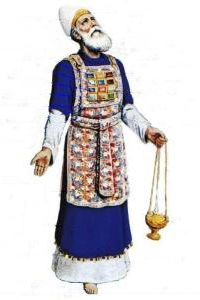
\includegraphics[width=50mm,scale=1.5]{Extras/Melchisedec.jpg}
\vspace{0.4in}  % Create a title for the document and write it in bold font
\LARGE{\textbf{\date}} % Again, do a line break
\linebreak 
% Create a subtitle \large{with Outlines, Statistics, Cross References, and Notes}
\vspace{0.5in}
\begin{flushleft}
\LARGE{Day \#48: Thursday, 17 February 2022 LITE\\} \vspace{0.25in}
\LARGE{Numbers 22-24 Psalm 48 Proverb 17}
\end{flushleft}
\vspace{0.6in}
\bigskip

\normalsize{Xenia, Oh.\\}
\normalsize{created: \today}
\vspace{1.3in}

\end{flushright}
\end{titlepage}

\newpage 
\tableofcontents\hypertarget{TOC}{}
\listoffigures
\listoftables

\hyphenation{A-bim-e-lech bre-thren E-phra-im  Gib-e-o-nites Jer-u-sa-lem through-out Phil-i-stines The-o-phil-us Am-a-le-kites ven-geance Mesh-el-e-mi-ah onan-ism Phar-a-oh thoughts grev-ous-ness Hach-a-liah adul-ter-er Shad-rach}

%%%%%%%%%%%%%%%%% EXTRA COLORS
%%%%%%%%%%%%%%%%% EXTRA COLORS
%%%%%%%%%%%%%%%%% EXTRA COLORS
\definecolor{champagne}{rgb}{0.97,0.91,0.81}
\definecolor{bone}{rgb}{0.89,0.85,0.79}

\definecolor{ForestGreen}{rgb}{0.00,0.29,0.098}
\definecolor{GIVING}{cmyk}{1,0.0,0.72,.1}

\definecolor{MLPE}{cmyk}{1,1,0,.45}
\definecolor{SOCCER}{cmyk}{.77, 0, .42, .49}
\definecolor{PAYBILL}{cmyk}{0,0.83,0.76,0.07}
\definecolor{SERMON}{cmyk}{.14,.9,0,.30} % aka seance \href{http://www.flatuicolorpicker.com/purple-cmyk-color-model/}{seance}
\definecolor{BIBLE}{cmyk}{0,.17,.74,.17}
\definecolor{WORKBLUE}{cmyk}{1, .5, 0, .6}
\definecolor{myOrange}{cmyk}{0, .4, .98, .03}
\definecolor{myTan}{cmyk}{0.0,.07,.17,.10}
\definecolor{myRed}{cmyk}{0,1,1,0}
\definecolor{myWhite}{cmyk}{0,0,0,0}
\definecolor{BLUESoD}{cmyk}{.97,.84,0,.04}
\definecolor{WHITE}{cmyk}{0,0,0,0}
\definecolor{OLDGOLD}{cmyk}{0.05,0.3,1.00,0}
\definecolor{CASTLETON}{cmyk}{1,0,0.31,0.66}
\definecolor{cadmiumgreen}{rgb}{0.0, 0.42, 0.24}
\definecolor{jungle}{rgb}{0.203,0.4882,0.1718}
\definecolor{MYGOLD}{rgb}{1,.84,0}

\definecolor{MYLIGHTGRAY}{rgb}{.85,.85,.85}

\definecolor{codegreen}{rgb}{0,0.6,0}
\definecolor{codegray}{rgb}{0.5,0.5,0.5}
\definecolor{codepurple}{rgb}{0.58,0,0.82}
\definecolor{backcolour}{rgb}{0.95,0.95,0.92}


\mdfdefinestyle{MyFrame}{%
    linecolor=blue,
    outerlinewidth=2pt,
    roundcorner=5pt,
    innertopmargin=\baselineskip,
    innerbottommargin=\baselineskip,
    innerrightmargin=10pt,
    innerleftmargin=10pt,
    backgroundcolor=gray!25!white}


\mdfdefinestyle{MyFrame2}{%
    linecolor=black,
    outerlinewidth=2pt,
    roundcorner=5pt,
    innertopmargin=\baselineskip,
    innerbottommargin=\baselineskip,
    innerrightmargin=10pt,
    innerleftmargin=10pt,
    backgroundcolor=yellow!25!white}


%%%%%
%% for PFTTIS list
%%%%%

%%% And Joseph said unto
\index[PFTTIS]{And Joseph said unto!Genesis!Gen 40:008}
\index[PFTTIS]{And Joseph said unto!Genesis!Gen 40:012}
\index[PFTTIS]{And Joseph said unto!Genesis!Gen 41:025}
\index[PFTTIS]{And Joseph said unto!Genesis!Gen 42:014}
\index[PFTTIS]{And Joseph said unto!Genesis!Gen 42:018}
\index[PFTTIS]{And Joseph said unto!Genesis!Gen 44:015}
\index[PFTTIS]{And Joseph said unto!Genesis!Gen 45:003}
\index[PFTTIS]{And Joseph said unto!Genesis!Gen 45:004}
\index[PFTTIS]{And Joseph said unto!Genesis!Gen 46:031}
\index[PFTTIS]{And Joseph said unto!Genesis!Gen 48:009}
\index[PFTTIS]{And Joseph said unto!Genesis!Gen 48:018}
\index[PFTTIS]{And Joseph said unto!Genesis!Gen 50:019}
\index[PFTTIS]{And Joseph said unto!Genesis!Gen 50:024}


%%% a shadow
\index[PFTTIS]{a shadow!1Chronicles!1Chr 029:15}
\index[PFTTIS]{a shadow!Job!Job 008:09}
\index[PFTTIS]{a shadow!Job!Job 014:02}
\index[PFTTIS]{a shadow!Job!Job 017:07}
\index[PFTTIS]{a shadow!Psalm!Psa 102:011}
\index[PFTTIS]{a shadow!Psalm!Psa 144:004}
\index[PFTTIS]{a shadow!Ecclesiastes!Eccl 006:012}
\index[PFTTIS]{a shadow!Ecclesiastes!Eccl 008:013}
\index[PFTTIS]{a shadow!Isaiah!Isa 04:006}
\index[PFTTIS]{a shadow!Isaiah!Isa 25:004}
\index[PFTTIS]{a shadow!Jonah!Jnh 04:06}
\index[PFTTIS]{a shadow!Colossians!Col 02:017}
\index[PFTTIS]{a shadow!Hebews!Heb 10:001}

%%% blessed is the man
\index[PFTTIS]{blessed is the man!Psalm!Psa 001:001}
\index[PFTTIS]{blessed is the man!Psalm!Psa 032:002}
\index[PFTTIS]{blessed is the man!Psalm!Psa 034:008}
\index[PFTTIS]{blessed is the man!Psalm!Psa 065:004}
\index[PFTTIS]{blessed is the man!Psalm!Psa 084:005}
\index[PFTTIS]{blessed is the man!Psalm!Psa 084:012}
\index[PFTTIS]{blessed is the man!Psalm!Psa 094:012}
\index[PFTTIS]{blessed is the man!Psalm!Psa 112:001}
\index[PFTTIS]{blessed is the man!Proverbs!Pro 008:034}
\index[PFTTIS]{blessed is the man!Isaiah!Isa 056:002}
\index[PFTTIS]{blessed is the man!Jeremiah!Jer 017:007}
\index[PFTTIS]{blessed is the man!Romans!Rom 004:008}
\index[PFTTIS]{blessed is the man!James!Jam 001:012}


%%% carry them
\index[PFTTIS]{carry them!Leviticus!Lev 14:045}
\index[PFTTIS]{carry them!Numbers!Num 11:012}
\index[PFTTIS]{carry them!Joshua!Jsh 04:003}
\index[PFTTIS]{carry them!1Samuel!1Sam 20:040}
\index[PFTTIS]{carry them!1Kings!1Kng 08:046}
\index[PFTTIS]{carry them!2Chronicles!2Chr 06:036}
\index[PFTTIS]{carry them!Ezra!Ezra 05:015}
\index[PFTTIS]{carry them!Isaiah!Isa 40:011}
\index[PFTTIS]{carry them!Isaiah!Isa 41:016}
\index[PFTTIS]{carry them!Isaiah!Isa 57:013}
\index[PFTTIS]{carry them!Jeremiah!Jer 20:004}
\index[PFTTIS]{carry them!Jeremiah!Jer 20:005}
\index[PFTTIS]{carry them!Jeremiah!Jer 43:012}


\index[PFTTIS]{good tidings!2Samuel!2Sam 18:027}
\index[PFTTIS]{good tidings!1Kings!1Ki 01:042}
\index[PFTTIS]{good tidings!2Kings!2Ki 07:009 (2x)}
\index[PFTTIS]{good tidings!Isaiah!Isa 40:009 (2x)}
\index[PFTTIS]{good tidings!Isaiah!Isa 41:007}
\index[PFTTIS]{good tidings!Isaiah!Isa 52:007}
\index[PFTTIS]{good tidings!Isaiah!Isa 61:001}
\index[PFTTIS]{good tidings!Nahum!Nah 01:005}
\index[PFTTIS]{good tidings!Luke!Lk 02:010}
\index[PFTTIS]{good tidings!1Thessalonians!1Thess 03:006}


%%% dead body
\index[PFTTIS]{dead body!Leviticus!Lev 21:011}
\index[PFTTIS]{dead body!Numbers!Num 06:006}
\index[PFTTIS]{dead body!Numbers!Num 09:006}
\index[PFTTIS]{dead body!Numbers!Num 09:007}
\index[PFTTIS]{dead body!Numbers!Num 09:010}
\index[PFTTIS]{dead body!Numbers!Num 09:011}
\index[PFTTIS]{dead body!Numbers!Num 09:013}
\index[PFTTIS]{dead body!Numbers!Num 09:016}
\index[PFTTIS]{dead body!2Kings!2Ki 08:005}
\index[PFTTIS]{dead body!Isaiah!Isa 26:019}
\index[PFTTIS]{dead body!Jeremiah!Jer 26:023}
\index[PFTTIS]{dead body!Jeremiah!Jer 36:030}
\index[PFTTIS]{dead body!Haggai!Hag 02:013}

%%% great sea
\index[PFTTIS]{great sea!Numbers!Num 34:006}
\index[PFTTIS]{great sea!Numbers!Num 34:007}
\index[PFTTIS]{great sea!Joshua!Jos 01:004}
\index[PFTTIS]{great sea!Joshua!Jos 09:001}
\index[PFTTIS]{great sea!Joshua!Jos 15:012}
\index[PFTTIS]{great sea!Joshua!Jos 15:047}
\index[PFTTIS]{great sea!Joshua!Jos 23:004}
\index[PFTTIS]{great sea!Ezekiel!Eze 47:010}
\index[PFTTIS]{great sea!Ezekiel!Eze 47:015}
\index[PFTTIS]{great sea!Ezekiel!Eze 47:019}
\index[PFTTIS]{great sea!Ezekiel!Eze 47:020}
\index[PFTTIS]{great sea!Ezekiel!Eze 48:028}
\index[PFTTIS]{great sea!Daniel!Dan 07:002}


%%% have forsaken me
\index[PFTTIS]{have forsaken me!Judges!Jdg 10:013}
\index[PFTTIS]{have forsaken me!1Samuel!1Sam 08:008}
\index[PFTTIS]{have forsaken me!1Kings!1Ki 11:033}
\index[PFTTIS]{have forsaken me!2Kings!2Ki 22:017}
\index[PFTTIS]{have forsaken me!2Chronicles!2Chr 12:005}
\index[PFTTIS]{have forsaken me!2Chronicles!2Chr 34:025}
\index[PFTTIS]{have forsaken me!Jeremiah!Jer 01:016}
\index[PFTTIS]{have forsaken me!Jeremiah!Jer 02:013}
\index[PFTTIS]{have forsaken me!Jeremiah!Jer 05:007}
\index[PFTTIS]{have forsaken me!Jeremiah!Jer 05:019}
\index[PFTTIS]{have forsaken me!Jeremiah!Jer 16:011 (2x)}
\index[PFTTIS]{have forsaken me!Jeremiah!Jer 19:004}

%%% no king
\index[PFTTIS]{no king!Judges!Jdg 17:06}
\index[PFTTIS]{no king!Judges!Jdg 18:01}
\index[PFTTIS]{no king!Judges!Jdg 19:01}
\index[PFTTIS]{no king!Judges!Jdg 21:25}
\index[PFTTIS]{no king!1Kings!1Ki 22:47}
\index[PFTTIS]{no king!2Kings!2Ki 23:25}
\index[PFTTIS]{no king!Nehemiah!Neh 13:26}
\index[PFTTIS]{no king!Psalms!Psa 033:016}
\index[PFTTIS]{no king!Proverbs!Pro 30:27}
\index[PFTTIS]{no king!Daniel!Dan 02:10}
\index[PFTTIS]{no king!Hosea!Hos 10:03}
\index[PFTTIS]{no king!Micah!Mic 04:09}
\index[PFTTIS]{no king!John!Jhn 19:15}


%%% rebellious house
\index[PFTTIS]{rebellious house!Exodus!Exo 02:005}
\index[PFTTIS]{rebellious house!Exodus!Exo 02:006}
\index[PFTTIS]{rebellious house!Exodus!Exo 02:008}
\index[PFTTIS]{rebellious house!Exodus!Exo 03:009}
\index[PFTTIS]{rebellious house!Exodus!Exo 03:026}
\index[PFTTIS]{rebellious house!Exodus!Exo 03:027}
\index[PFTTIS]{rebellious house!Exodus!Exo 12:002 (2x)}
\index[PFTTIS]{rebellious house!Exodus!Exo 12:003}
\index[PFTTIS]{rebellious house!Exodus!Exo 12:009}
\index[PFTTIS]{rebellious house!Exodus!Exo 12:025}
\index[PFTTIS]{rebellious house!Exodus!Exo 17:012}
\index[PFTTIS]{rebellious house!Exodus!Exo 24:003}

%%% seek him
\index[PFTTIS]{seek him!Deuteronomy!Deu 04:029}\index[PFTTIS]{seek him!1Samuel!1Sam 23:025}
\index[PFTTIS]{seek him!1Chronicles!1Chr 28:009}
\index[PFTTIS]{seek him!2Chronicles!1Chr 15:002}
\index[PFTTIS]{seek him!Ezra!Ezr 08:022}
\index[PFTTIS]{seek him!Psalms!Psa 022:026}
\index[PFTTIS]{seek him!Psalms!Psa 024:006}
\index[PFTTIS]{seek him!Psalms!Psa 119:002}
\index[PFTTIS]{seek him!SoS!SoS 03:002}
\index[PFTTIS]{seek him!SoS!SoS 06:001}
\index[PFTTIS]{seek him!Hosea!Hos 07:010}
\index[PFTTIS]{seek him!Amos!Amo 05:008}
\index[PFTTIS]{seek him!Hebrews!Heb 11:0063}


%%% seek ye
\index[PFTTIS]{seek ye!Isaiah!Isa 34:016}
\index[PFTTIS]{seek ye!Isaiah!Isa 45:019}
\index[PFTTIS]{seek ye!Isaiah!Isa 55:006}
\index[PFTTIS]{seek ye!Amos!Amos 5:004}
\index[PFTTIS]{seek ye!John!John 1:38}
\index[PFTTIS]{seek ye!John!John 18:4}
\index[PFTTIS]{seek ye!John!John 18:7}
\index[PFTTIS]{seek ye!Matthew!Matt 6:33}
\index[PFTTIS]{seek ye!Numbers!Num 16:10}
\index[PFTTIS]{seek ye!Luke!Luke 12:31}
\index[PFTTIS]{seek ye!Luke!Luke 24:5}
\index[PFTTIS]{seek ye!Psalm!Psa 27:8}
\index[PFTTIS]{seek ye!Zephaniah!Zeph 2:3}

%%% the uncircumcised
\index[PFTTIS]{the uncircumcised!Genesis!Gen 17:014}
\index[PFTTIS]{the uncircumcised!Judges!Jdg 14:003}
\index[PFTTIS]{the uncircumcised!Judges!Jdg 15:018}
\index[PFTTIS]{the uncircumcised!2Samuel!2Sam 01:020}
\index[PFTTIS]{the uncircumcised!Isaiah!Isa 02:001}
\index[PFTTIS]{the uncircumcised!Jeremiah!Jer 09:025}
\index[PFTTIS]{the uncircumcised!Ezekiel!Eze 28:010}
\index[PFTTIS]{the uncircumcised!Ezekiel!Eze 31:018}
\index[PFTTIS]{the uncircumcised!Ezekiel!Eze 32:019}
\index[PFTTIS]{the uncircumcised!Ezekiel!Eze 32:027}
\index[PFTTIS]{the uncircumcised!Ezekiel!Eze 32:028}
\index[PFTTIS]{the uncircumcised!Ezekiel!Eze 32:029}
\index[PFTTIS]{the uncircumcised!Ezekiel!Eze 32:032}

%%% worship him
\index[PFTTIS]{worship him!Psalms!Psa 97:007}
\index[PFTTIS]{worship him!Zephaniah!Zeph 02:011}
\index[PFTTIS]{worship him!Matthew!Matt 02:002}
\index[PFTTIS]{worship him!Matthew!Matt 02:008}
\index[PFTTIS]{worship him!John!John 04:023}
\index[PFTTIS]{worship him!John!John 04:024 (2x)} 
\index[PFTTIS]{worship him!Acts!Acts 17:023}
\index[PFTTIS]{worship him!Hebrews!Heb 01:006}
\index[PFTTIS]{worship him!Revelation!Rev 04:010}
\index[PFTTIS]{worship him!Revelation!Rev 13:008}
\index[PFTTIS]{worship him!Revelation!Rev 14:007}
\index[PFTTIS]{worship him!Revelation!Rev 19:010}


%%%%%
%% for PFTTIS list
%%%%%

%%% afflictions
\index[WFTTIS]{afflictions!Psalms!Psa 34:019}
\index[WFTTIS]{afflictions!Psalms!Psa 132:001}
\index[WFTTIS]{afflictions!Acts!Acts 07:010}
\index[WFTTIS]{afflictions!Acts!Acts 20:023}
\index[WFTTIS]{afflictions!2Corinthians!2Cor 06:004}
\index[WFTTIS]{afflictions!Colossians!Col 01:024}
\index[WFTTIS]{afflictions!1Thessalonians!1Thess 03:003}
\index[WFTTIS]{afflictions!2Timothy!2Tim 01:008}
\index[WFTTIS]{afflictions!2Timothy!2Tim 03:011}
\index[WFTTIS]{afflictions!2Timothy!2Tim 04:005}
\index[WFTTIS]{afflictions!Hebrews!Heb 10:032}
\index[WFTTIS]{afflictions!Hebrews!Heb 10:033}
\index[WFTTIS]{afflictions!1Peter!1Pet 05:009}

%%% acsend
\index[WFTTIS]{acsend!Joshua!Jos 06:05}
\index[WFTTIS]{acsend!Psalm!Psa 024:003}
\index[WFTTIS]{acsend!Psalm!Psa 135:007}
\index[WFTTIS]{acsend!Psalm!Psa 139:008}
\index[WFTTIS]{acsend!Isaiah!Isa 14:013}
\index[WFTTIS]{acsend!Isaiah!Isa 14:014}
\index[WFTTIS]{acsend!Jeremiah!Jer 10:013}
\index[WFTTIS]{acsend!Jeremiah!Jer 51:016}
\index[WFTTIS]{acsend!Ezekiel!Eze 38:009}
\index[WFTTIS]{acsend!John!John 06:062}
\index[WFTTIS]{acsend!John!John 20:017}
\index[WFTTIS]{acsend!Romans!Rom 10:006}
\index[WFTTIS]{acsend!Revelation!Rev 17:008}

%%% Assyrian
\index[WFTTIS]{Assyrian!Isaiah!Isa 10:005}
\index[WFTTIS]{Assyrian!Isaiah!Isa 10:024}
\index[WFTTIS]{Assyrian!Isaiah!Isa 14:025}
\index[WFTTIS]{Assyrian!Isaiah!Isa 19:023}
\index[WFTTIS]{Assyrian!Isaiah!Isa 23:013}
\index[WFTTIS]{Assyrian!Isaiah!Isa 30:031}
\index[WFTTIS]{Assyrian!Isaiah!Isa 31:008}
\index[WFTTIS]{Assyrian!Isaiah!Isa 52:004}
\index[WFTTIS]{Assyrian!Ezekiel!Eze 31:003}
\index[WFTTIS]{Assyrian!Hosea!Hos 05:013}
\index[WFTTIS]{Assyrian!Hosea!Hos 11:005}
\index[WFTTIS]{Assyrian!Micah!Hos 05:005}
\index[WFTTIS]{Assyrian!Micah!Hos 05:006}

%%% blot
\index[WFTTIS]{blot!Exodus!Exo 32:032}
\index[WFTTIS]{blot!Exodus!Exo 32:033}
\index[WFTTIS]{blot!Numbers!Num 05:026}
\index[WFTTIS]{blot!Deuteronomy!Deut 09:014}
\index[WFTTIS]{blot!Deuteronomy!Deut 25:019}
\index[WFTTIS]{blot!Deuteronomy!Deut 29:020}
\index[WFTTIS]{blot!2Kings!2Ki 14:027}
\index[WFTTIS]{blot!Job!Job 31:007}
\index[WFTTIS]{blot!Psalms!Psa 51:001}
\index[WFTTIS]{blot!Psalms!Psa 51:009}
\index[WFTTIS]{blot!Proverbs!Pro 09:007}
\index[WFTTIS]{blot!Jeremiah!Jer 18:023}
\index[WFTTIS]{blot!Revelation!Rev 03:005}


%%% chain
\index[WFTTIS]{chain!Genesis!Gen 41:042}
\index[WFTTIS]{chain!1Kings!1Ki 07:017}
\index[WFTTIS]{chain!Psalms!Psa 73:006}
\index[WFTTIS]{chain!SoS!Sos 04:009}
\index[WFTTIS]{chain!Lamentations!Lam 03:007}
\index[WFTTIS]{chain!Ezekiel!Eze 07:023}
\index[WFTTIS]{chain!Ezekiel!Eze 16:011}
\index[WFTTIS]{chain!Daniel!Dan 05:007}
\index[WFTTIS]{chain!Daniel!Dan 05:016}
\index[WFTTIS]{chain!Daniel!Dan 05:029}
\index[WFTTIS]{chain!Acts!Acts 28:020}
\index[WFTTIS]{chain!2Timothy!2Tim 01:016}
\index[WFTTIS]{chain!Revelation!Rev 20:001}


%%% controversy
\index[WFTTIS]{controversy!Deuteronomy!Deu 17:008}
\index[WFTTIS]{controversy!Deuteronomy!Deu 19:017}
\index[WFTTIS]{controversy!Deuteronomy!Deu 21:005}
\index[WFTTIS]{controversy!Deuteronomy!Deu 25:001}
\index[WFTTIS]{controversy!2Samuel!2Sam 15:002}
\index[WFTTIS]{controversy!Isaiah!Isa 34:008}
\index[WFTTIS]{controversy!Jeremiah!Jer 25:031}
\index[WFTTIS]{controversy!Ezekiel!Eze 44:024}
\index[WFTTIS]{controversy!Hosea!Hos 04:001}
\index[WFTTIS]{controversy!Hosea!Hos 12:002}
\index[WFTTIS]{controversy!Micah!Mic 06:002 (2x)}
\index[WFTTIS]{controversy!1Timothy!1Tim 03:016}


%%% Dagon/Dagon's
\index[WFTTIS]{Dagon!Judges!Jdg 16:023}
\index[WFTTIS]{Dagon!1Samuel!1Sam 05:002 (2x)}
\index[WFTTIS]{Dagon!1Samuel!1Sam 05:003 (2x)}
\index[WFTTIS]{Dagon!1Samuel!1Sam 05:004 (3x)}
\index[WFTTIS]{Dagon!1Samuel!1Sam 05:005 (3x)}
\index[WFTTIS]{Dagon!1Samuel!1Sam 05:007}
\index[WFTTIS]{Dagon!1Chronicles!1Chr 10:010}

%%% disobedient
\index[WFTTIS]{disobedient!1Kings!1Ki 13:026}
\index[WFTTIS]{disobedient!Nehemiah!Neh 09:026}
\index[WFTTIS]{disobedient!Luke!Luke 01:017}
\index[WFTTIS]{disobedient!Acts!Acts 26:019}
\index[WFTTIS]{disobedient!Romans!Rom 01:030}
\index[WFTTIS]{disobedient!Romans!Rom 10:021}
\index[WFTTIS]{disobedient!1Timothy!1Tim 01:009}
\index[WFTTIS]{disobedient!2Timothy!2Tim 03:002}
\index[WFTTIS]{disobedient!Titus!Titus 01:016}
\index[WFTTIS]{disobedient!Titus!Titus 03:003}
\index[WFTTIS]{disobedient!1Peter!1Pet 02:007}
\index[WFTTIS]{disobedient!1Peter!1Pet 02:008}
\index[WFTTIS]{disobedient!1Peter!1Pet 03:020}


%%% doubt
\index[WFTTIS]{doubt!Genesis!Gen 37:033}
\index[WFTTIS]{doubt!Deuteronomy!Deu 28:066}
\index[WFTTIS]{doubt!Job!Job 12:002}
\index[WFTTIS]{doubt!Matthew!Matt 14:031}
\index[WFTTIS]{doubt!Matthew!Matt 21:021}
\index[WFTTIS]{doubt!Mark!Mk 11:023}
\index[WFTTIS]{doubt!Luke!Lk 11:020}
\index[WFTTIS]{doubt!John!Jhn 10:024}
\index[WFTTIS]{doubt!Acts!Acts 02:012}
\index[WFTTIS]{doubt!Acts!Acts 28:004}
\index[WFTTIS]{doubt!1Corinthians!1Cor 09:010}
\index[WFTTIS]{doubt!Galatians!Gal 04:020}
\index[WFTTIS]{doubt!1John!1Jhn 02:019}


%%% dungeon
\index[WFTTIS]{dungeon!Genesis!Gen 40:015}
\index[WFTTIS]{dungeon!Genesis!Gen 41:014}
\index[WFTTIS]{dungeon!Exodus!Exo 12:029}
\index[WFTTIS]{dungeon!Jeremiah!Jer 37:016}
\index[WFTTIS]{dungeon!Jeremiah!Jer 38:006 (2x)}
\index[WFTTIS]{dungeon!Jeremiah!Jer 38:007}
\index[WFTTIS]{dungeon!Jeremiah!Jer 38:009}
\index[WFTTIS]{dungeon!Jeremiah!Jer 38:010}
\index[WFTTIS]{dungeon!Jeremiah!Jer 38:011}
\index[WFTTIS]{dungeon!Jeremiah!Jer 38:013}
\index[WFTTIS]{dungeon!Lamentations!Lam 03:053}
\index[WFTTIS]{dungeon!Lamentations!Lam 03:055}


%%% error
\index[WFTTIS]{error!2Samuel!2Sam 06:007}
\index[WFTTIS]{error!Job!Job 19:004}
\index[WFTTIS]{error!Ecclesiastes!Ecc 05:006}
\index[WFTTIS]{error!Ecclesiastes!Ecc 10:005}
\index[WFTTIS]{error!Isaiah!Isa 32:006}
\index[WFTTIS]{error!Daniel!Dan 06:004}
\index[WFTTIS]{error!Matthew!Matt 27:064}
\index[WFTTIS]{error!Romans!Rom 01:027}
\index[WFTTIS]{error!James!Jam 05:020}
\index[WFTTIS]{error!2Peter!2Pet 02:018}
\index[WFTTIS]{error!2Peter!2Pet 03:017}
\index[WFTTIS]{error!1John!1Jn 04:006}
\index[WFTTIS]{error!Jude!Jude 01:011}

%%% fourish
\index[WFTTIS]{fourish!Psalms!Psa 072:007}
\index[WFTTIS]{fourish!Psalms!Psa 072:016}
\index[WFTTIS]{fourish!Psalms!Psa 092:007}
\index[WFTTIS]{fourish!Psalms!Psa 092:012}
\index[WFTTIS]{fourish!Psalms!Psa 092:013}
\index[WFTTIS]{fourish!Psalms!Psa 132:018}
\index[WFTTIS]{fourish!Proverbs!Pro 11:28}
\index[WFTTIS]{fourish!Proverbs!Pro 14:11}
\index[WFTTIS]{fourish!Ecclesiastes!Ecc 12:05}
\index[WFTTIS]{fourish!SongOfSolomon!SOS 07:12}
\index[WFTTIS]{fourish!Isaiah!Isa 17:11}
\index[WFTTIS]{fourish!Isaiah!Isa 66:14}
\index[WFTTIS]{fourish!Ezekiel!Eze 17:24}




%%% giants
\index[WFTTIS]{giants!Genesis!Gen 06:004}
\index[WFTTIS]{giants!Numbers!Num 13:033}
\index[WFTTIS]{giants!Deuteronomy!Deut 02:011}
\index[WFTTIS]{giants!Deuteronomy!Deut 02:021}
\index[WFTTIS]{giants!Deuteronomy!Deut 03:011}
\index[WFTTIS]{giants!Deuteronomy!Deut 03:013}
\index[WFTTIS]{giants!Joshua!Josh 12:004}
\index[WFTTIS]{giants!Joshua!Josh 13:012}
\index[WFTTIS]{giants!Joshua!Josh 15:008}
\index[WFTTIS]{giants!Joshua!Josh 17:015}
\index[WFTTIS]{giants!Joshua!Josh 16:016}

%%% good man
\index[WFTTIS]{good man!2 Samuel!2Sa 18:27}
%(1) Psalms 37:23 [5]
%(1) Psalms 112:5 [2]
%(1) Proverbs 12:2 [2]
%(1) Proverbs 13:22 [2]
%(1) Proverbs 14:14 [14]
%(1) Micah 7:2 [2]
%(1) Matthew 12:35 [2]
%(1) Luke 6:45 [2]
%(1) Luke 23:50 [15]
%(1) John 7:12 [17]
%(1) Acts 11:24 [5]
%(1) Romans 5:7 [14]

%%% Hinnom
\index[WFTTIS]{Hinnom!Joshua!Jsh 15:008}
\index[WFTTIS]{Hinnom!Joshua!Jsh 18:016}
\index[WFTTIS]{Hinnom!2Kings!2Ki 23:010}
\index[WFTTIS]{Hinnom!2Chronicles!2Chr 28:003}
\index[WFTTIS]{Hinnom!2Chronicles!2Chr 33:006}
\index[WFTTIS]{Hinnom!Nehemiah!Neh 11:030}
\index[WFTTIS]{Hinnom!Jeremiah!Jer 07:031}
\index[WFTTIS]{Hinnom!Jeremiah!Jer 07:032}
\index[WFTTIS]{Hinnom!Jeremiah!Jer 19:002}
\index[WFTTIS]{Hinnom!Jeremiah!Jer 19:006}
\index[WFTTIS]{Hinnom!Jeremiah!Jer 32:035}

%%% inclined
\index[WFTTIS]{inclined!Judges!Jdg 09:003}
\index[WFTTIS]{inclined!Psalms!Psa 040:001}
\index[WFTTIS]{inclined!Psalms!Psa 116:002}
\index[WFTTIS]{inclined!Psalms!Psa 119:112}
\index[WFTTIS]{inclined!Proverbs!Pro 05:13}
\index[WFTTIS]{inclined!Jeremiah!Jer 07:24}
\index[WFTTIS]{inclined!Jeremiah!Jer 07:26}
\index[WFTTIS]{inclined!Jeremiah!Jer 11:08}
\index[WFTTIS]{inclined!Jeremiah!Jer 17:23}
\index[WFTTIS]{inclined!Jeremiah!Jer 25:04}
\index[WFTTIS]{inclined!Jeremiah!Jer 34:14}
\index[WFTTIS]{inclined!Jeremiah!Jer 35:15}
\index[WFTTIS]{inclined!Jeremiah!Jer 44:05}


%%% laughed
\index[WFTTIS]{laughed!Genesis!Gen 17:017}
\index[WFTTIS]{laughed!Genesis!Gen 18:012}
\index[WFTTIS]{laughed!Genesis!Gen 18:015}
\index[WFTTIS]{laughed!2Kings!2Ki 19:021}
\index[WFTTIS]{laughed!2Chronicles!2Chr 30:010}
\index[WFTTIS]{laughed!Nehemiah!Neh 02:019}
\index[WFTTIS]{laughed!Job!Job 12:004}
\index[WFTTIS]{laughed!Job!Job 29:024}
\index[WFTTIS]{laughed!Isaiah!Isa 37:022}
\index[WFTTIS]{laughed!Ezekiel!Ezek 23:032}
\index[WFTTIS]{laughed!Matthew!Matt 09:024}
\index[WFTTIS]{laughed!Mark!Mk 05:040}
\index[WFTTIS]{laughed!Luke!Lk 08:053}

%%% liar
\index[WFTTIS]{liar!Job!Job 24:025}
\index[WFTTIS]{liar!Proverbs!Pro 17:004}
\index[WFTTIS]{liar!Proverbs!Pro 19:022}
\index[WFTTIS]{liar!Proverbs!Pro 30:006}
\index[WFTTIS]{liar!Jeremiah!Jer 15:018}
\index[WFTTIS]{liar!John!Jhn 08:044}
\index[WFTTIS]{liar!John!Jhn 08:055}
\index[WFTTIS]{liar!Romans!Rom 03:004}
\index[WFTTIS]{liar!1John!1Jhn 01:010}
\index[WFTTIS]{liar!1John!1Jhn 02:004}
\index[WFTTIS]{liar!1John!1Jhn 02:022}
\index[WFTTIS]{liar!1John!1Jhn 04:020}
\index[WFTTIS]{liar!1John!1Jhn 05:010}

%%% palsy
\index[WFTTIS]{palsy!Matthew!Matt 04:024}
\index[WFTTIS]{palsy!Matthew!Matt 08:006}
\index[WFTTIS]{palsy!Matthew!Matt 09:002}
\index[WFTTIS]{palsy!Matthew!Matt 09:006}
\index[WFTTIS]{palsy!Mark!Mk 02:003}
\index[WFTTIS]{palsy!Mark!Mk 02:004}
\index[WFTTIS]{palsy!Mark!Mk 02:005}
\index[WFTTIS]{palsy!Mark!Mk 02:009}
\index[WFTTIS]{palsy!Mark!Mk 02:010}
\index[WFTTIS]{palsy!Luke!Lk 05:018}
\index[WFTTIS]{palsy!Luke!Lk 05:024}
\index[WFTTIS]{palsy!Acts!Acts 09:033}

%%% Profitable
\index[WFTTIS]{profitable!Job!Job 22:002 (2x)}
\index[WFTTIS]{profitable!Ecclesiastes!Ecc 10:010}
\index[WFTTIS]{profitable!Isaiah!Isa 44:010}
\index[WFTTIS]{profitable!Jeremiah!Jer 13:007}
\index[WFTTIS]{profitable!Matthew!Matt 05:029}
\index[WFTTIS]{profitable!Matthew!Matt 05:030}
\index[WFTTIS]{profitable!Acts!Acts 20:020}
\index[WFTTIS]{profitable!1Timothy!1Tim 04:008}
\index[WFTTIS]{profitable!2Timothy!2Tim 03:016}
\index[WFTTIS]{profitable!2Timothy!2Tim 04:011}
\index[WFTTIS]{profitable!Titus!Titus 03:008}
\index[WFTTIS]{profitable!Philemon!Phlm 01:011}

%%% Rechab
\index[WFTTIS]{Rechab!2Samuel!2Sam 04:002}
\index[WFTTIS]{Rechab!2Samuel!2Sam 04:005}
\index[WFTTIS]{Rechab!2Samuel!2Sam 04:006}
\index[WFTTIS]{Rechab!2Samuel!2Sam 04:009}
\index[WFTTIS]{Rechab!2KIngs!2Ki 10:015}
\index[WFTTIS]{Rechab!2KIngs!2Ki 10:023}
\index[WFTTIS]{Rechab!1Chronicles!1Chr 02:055}
\index[WFTTIS]{Rechab!Nehemiah!Neh 03:014}
\index[WFTTIS]{Rechab!Jeremiah!Jer 35:006}
\index[WFTTIS]{Rechab!Jeremiah!Jer 35:008}
\index[WFTTIS]{Rechab!Jeremiah!Jer 35:014}
\index[WFTTIS]{Rechab!Jeremiah!Jer 35:016}
\index[WFTTIS]{Rechab!Jeremiah!Jer 35:019}

%%% serpents
\index[WFTTIS]{serpents!Exodus!Exo 07:012}
\index[WFTTIS]{serpents!Numbers!Num 21:006}
\index[WFTTIS]{serpents!Numbers!Num 21:007}
\index[WFTTIS]{serpents!Deuteronomy!Deu 08:015}
\index[WFTTIS]{serpents!Deuteronomy!Deu 32:024}
\index[WFTTIS]{serpents!Jeremiah!Jer 08:017}
\index[WFTTIS]{serpents!Matthew!Matt 10:016}
\index[WFTTIS]{serpents!Matthew!Matt 23:033}
\index[WFTTIS]{serpents!Mark!Mk 16:018}
\index[WFTTIS]{serpents!Luke!Lk 10:019}
\index[WFTTIS]{serpents!1Corinthians!1Cor 10:009}
\index[WFTTIS]{serpents!James!Jas 03:007}
\index[WFTTIS]{serpents!Revelation!Rev 09:019}

%%% short
\index[WFTTIS]{short!Numbers!Num 11:023}
\index[WFTTIS]{short!2Kings!2Ki 10:032}
\index[WFTTIS]{short!Job!Job 17:012}
\index[WFTTIS]{short!Job!Job 20:005}
\index[WFTTIS]{short!Psalms!Psa 89:047}
\index[WFTTIS]{short!Romans!Rom 03:023}
\index[WFTTIS]{short!Romans!Rom 09:028  (2x)}
\index[WFTTIS]{short!1Corinthians!1Cor 07:029}
\index[WFTTIS]{short!1Thessalonians!1Thess 02:017}
\index[WFTTIS]{short!Hebrews!Heb 04:001}
\index[WFTTIS]{short!Revelation!Rev 12:012}
\index[WFTTIS]{short!Revelation!Rev 17:010}

%%% smiteth
\index[WFTTIS]{smiteth!Exodus!Exo 21:012}
\index[WFTTIS]{smiteth!Exodus!Exo 21:15}
\index[WFTTIS]{smiteth!Deuteronomy!Dt 25:11}
\index[WFTTIS]{smiteth!Deuteronomy!Dt 27:24}
\index[WFTTIS]{smiteth!Joshua!Jsh 15:16}
\index[WFTTIS]{smiteth!Judges!Jdg 15:16}
\index[WFTTIS]{smiteth!2 Samuel!2Sa 05:08}
\index[WFTTIS]{smiteth!1Chronicles!1Chr 11:06}
\index[WFTTIS]{smiteth!Job!1Chr 26:12}
\index[WFTTIS]{smiteth!Isaiah!Isa 09:13}
\index[WFTTIS]{smiteth!Lamentations!Lam 03:30}
\index[WFTTIS]{smiteth!Ezekiel!Eze 07:09}
\index[WFTTIS]{smiteth!Luke!Lk 06:29}



%%% vanities
\index[WFTTIS]{vanities!Deuteronomy!Deut 21:021}
\index[WFTTIS]{vanities!1Kings!1Ki 16:013}
\index[WFTTIS]{vanities!1Kings!1Ki 16:026}
\index[WFTTIS]{vanities!Psalms!Psa 031:006}
\index[WFTTIS]{vanities!Ecclesiastes!Ecc 01:002 (2x)}
\index[WFTTIS]{vanities!Ecclesiastes!Ecc 05:007}
\index[WFTTIS]{vanities!Ecclesiastes!Ecc 12:008}
\index[WFTTIS]{vanities!Jeremiah!Jer 08:019}
\index[WFTTIS]{vanities!Jeremiah!Jer 10:008}
\index[WFTTIS]{vanities!Jeremiah!Jer 14:022}
\index[WFTTIS]{vanities!Jonah!Jnh 02:008}
\index[WFTTIS]{vanities!Acts!Acts 14:015}



%%%%%
%% for PFTTIS list
%%%%%

%%% worm
\index[WFITV]{worm!Exodus!Exo 16:024}
\index[WFITV]{worm!Job!Job 17:014}
\index[WFITV]{worm!Job!Job 24:029}
\index[WFITV]{worm!Job!Job 25:005 (2x)}
\index[WFITV]{worm!Psalms!Psa 022:006}
\index[WFITV]{worm!Isaiah!Isa 14:011}
\index[WFITV]{worm!Isaiah!Isa 41:014}
\index[WFITV]{worm!Isaiah!Isa 51:008}
\index[WFITV]{worm!Isaiah!Isa 66:024}
\index[WFITV]{worm!Jonah!Jnh 04:007}
\index[WFITV]{worm!Mark!Mk 09:044}
\index[WFITV]{worm!Mark!Mk 09:046}
\index[WFITV]{worm!Mark!Mk 09:048}


%\subsubsection{Title}
%\textbf{Introduction:} Isaiah 46 
%\index[speaker]{Speaker!Isaiah 49 (Title}
%\index[series]{Book (Speaker)!IPassage (Title)}
%\index[date]{2017/07/09!Isaiah 49 (Title)}
%\begin{compactenum}[I.]
%    \item  \textbf{Point} \index[scripture]{Isaiah!IPassage} (IPassage)
%\end{compactenum}




  


%\input{02OT-Exodus/ExodusIntroduction}
\newpage
\begin{figure}
\begin{center}
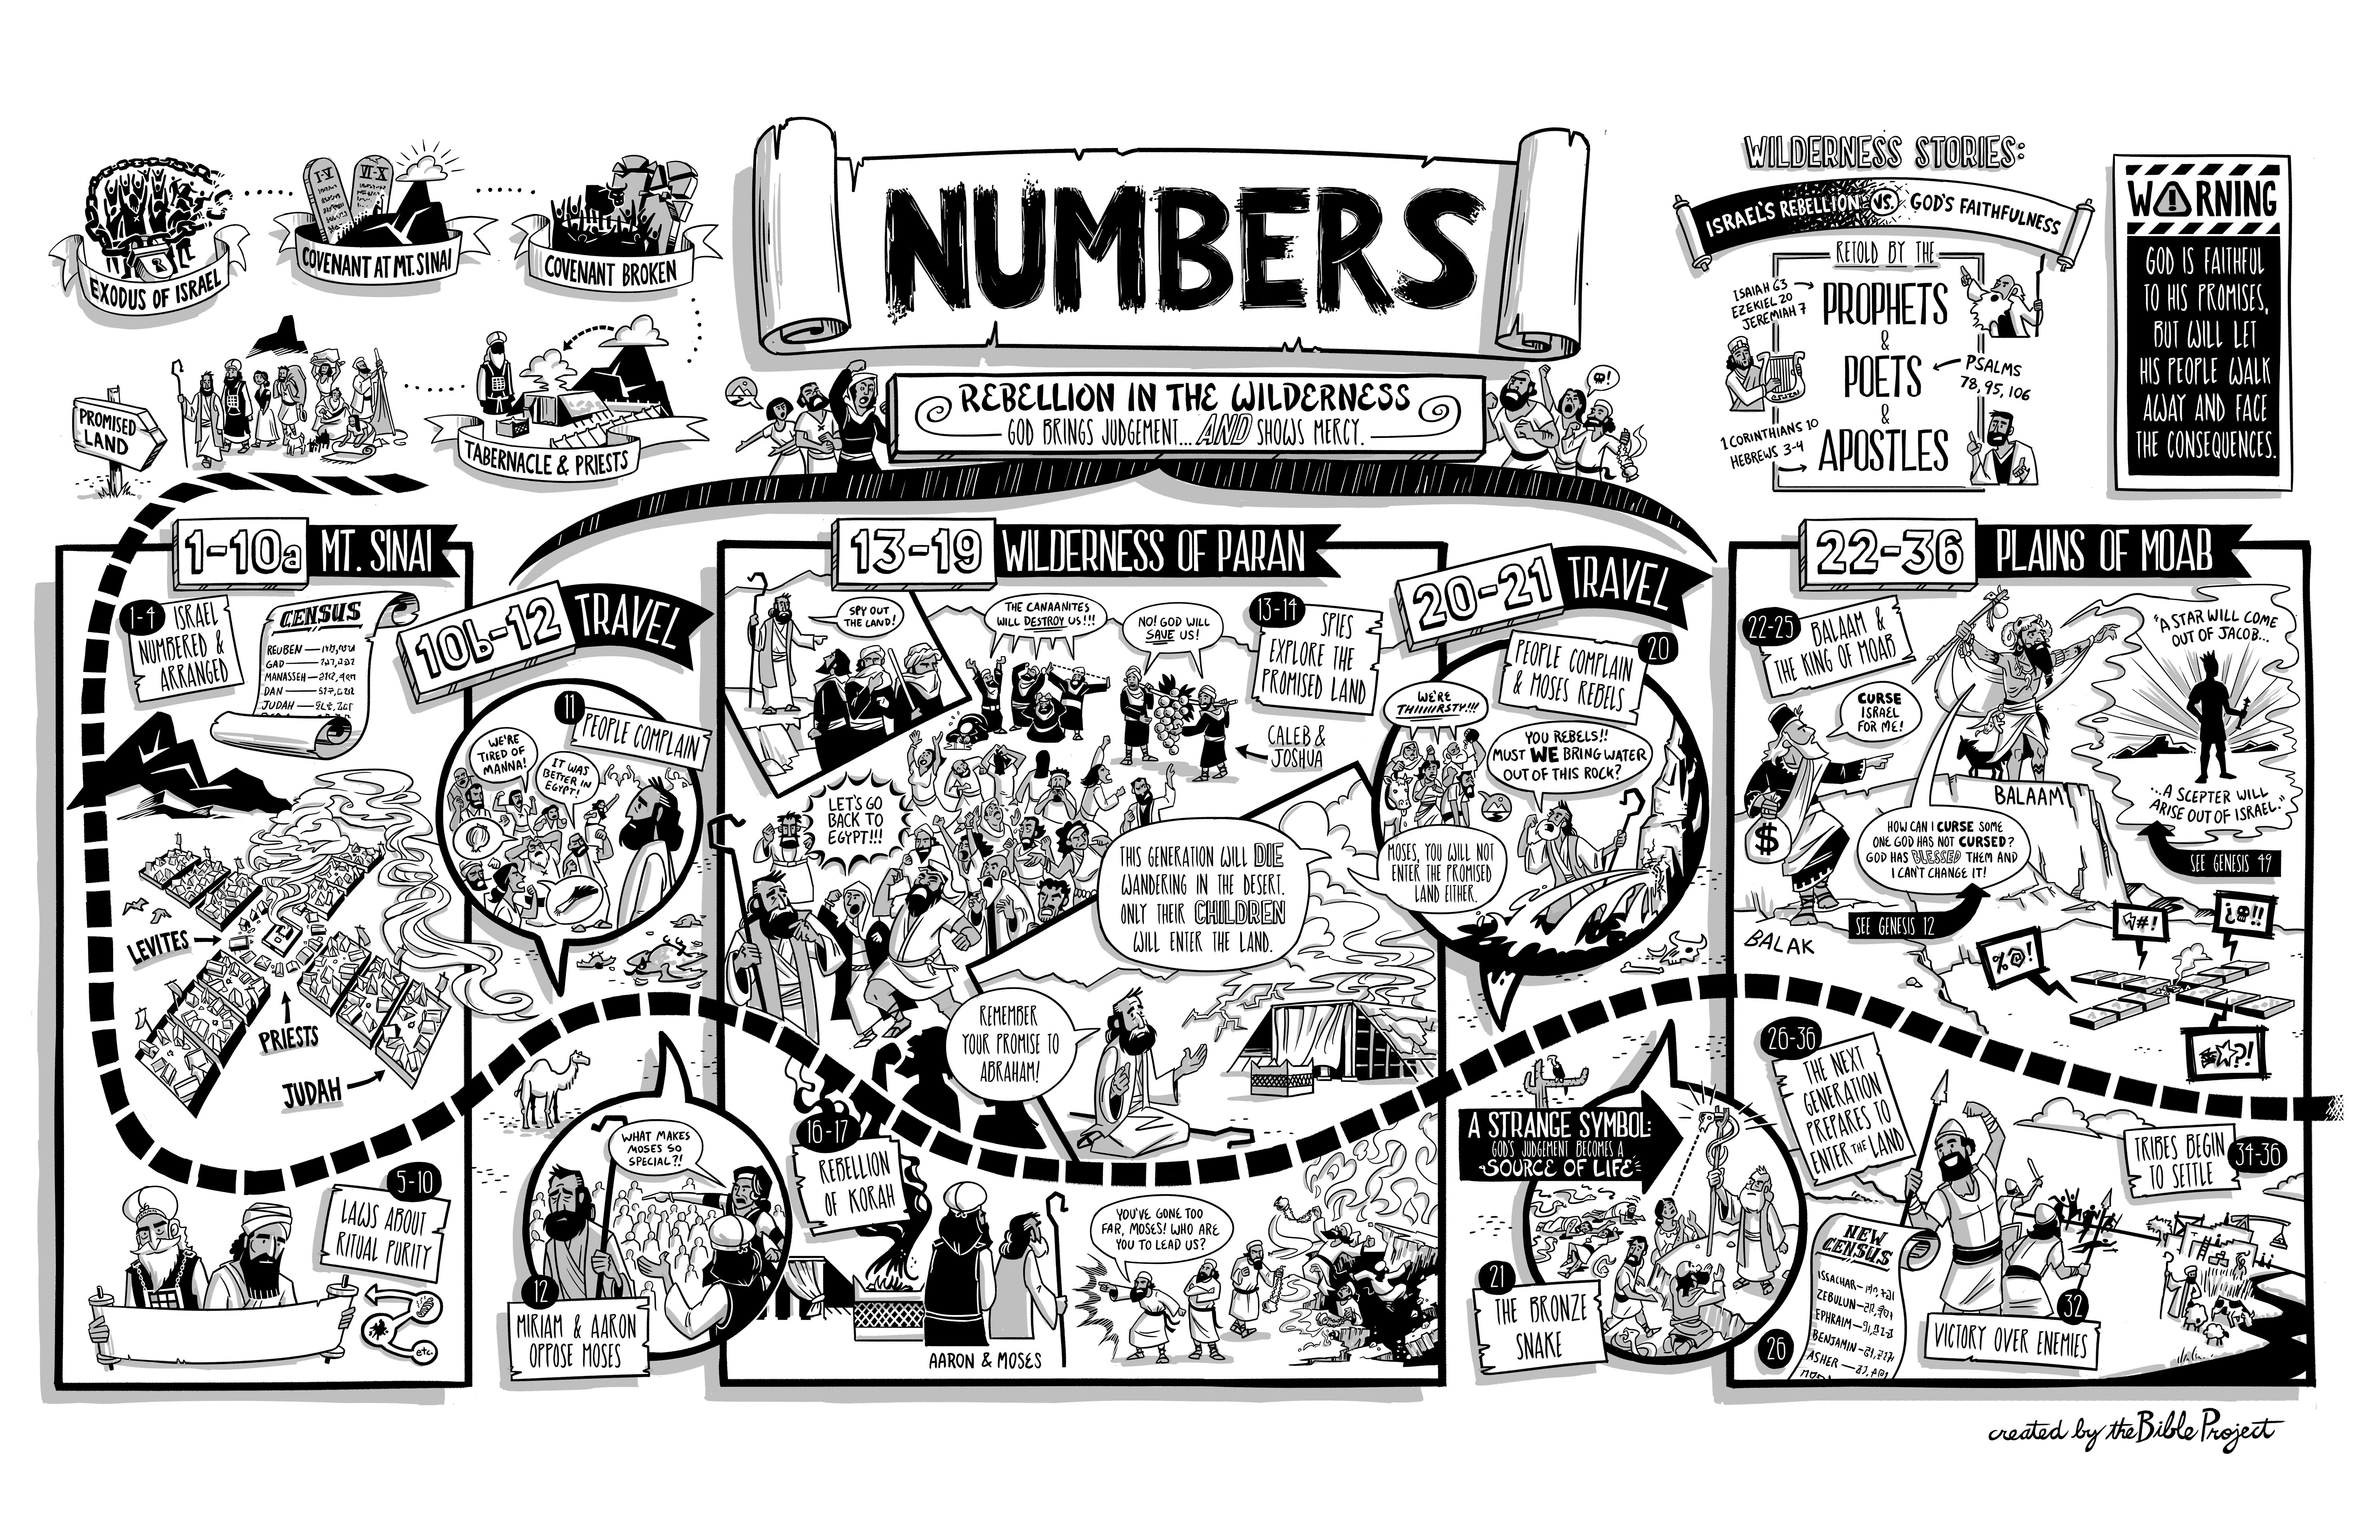
\includegraphics[scale=0.5, angle=90]{04OT-Numbers/References/BibleProject-Numbers.jpg}
\caption[Numbers from the Bible Project]{Numbers from the Bible Project}
\label{fig:Numbers from the Bible Project}
\end{center}
\end{figure}

\newpage
\begin{figure}
\begin{center}
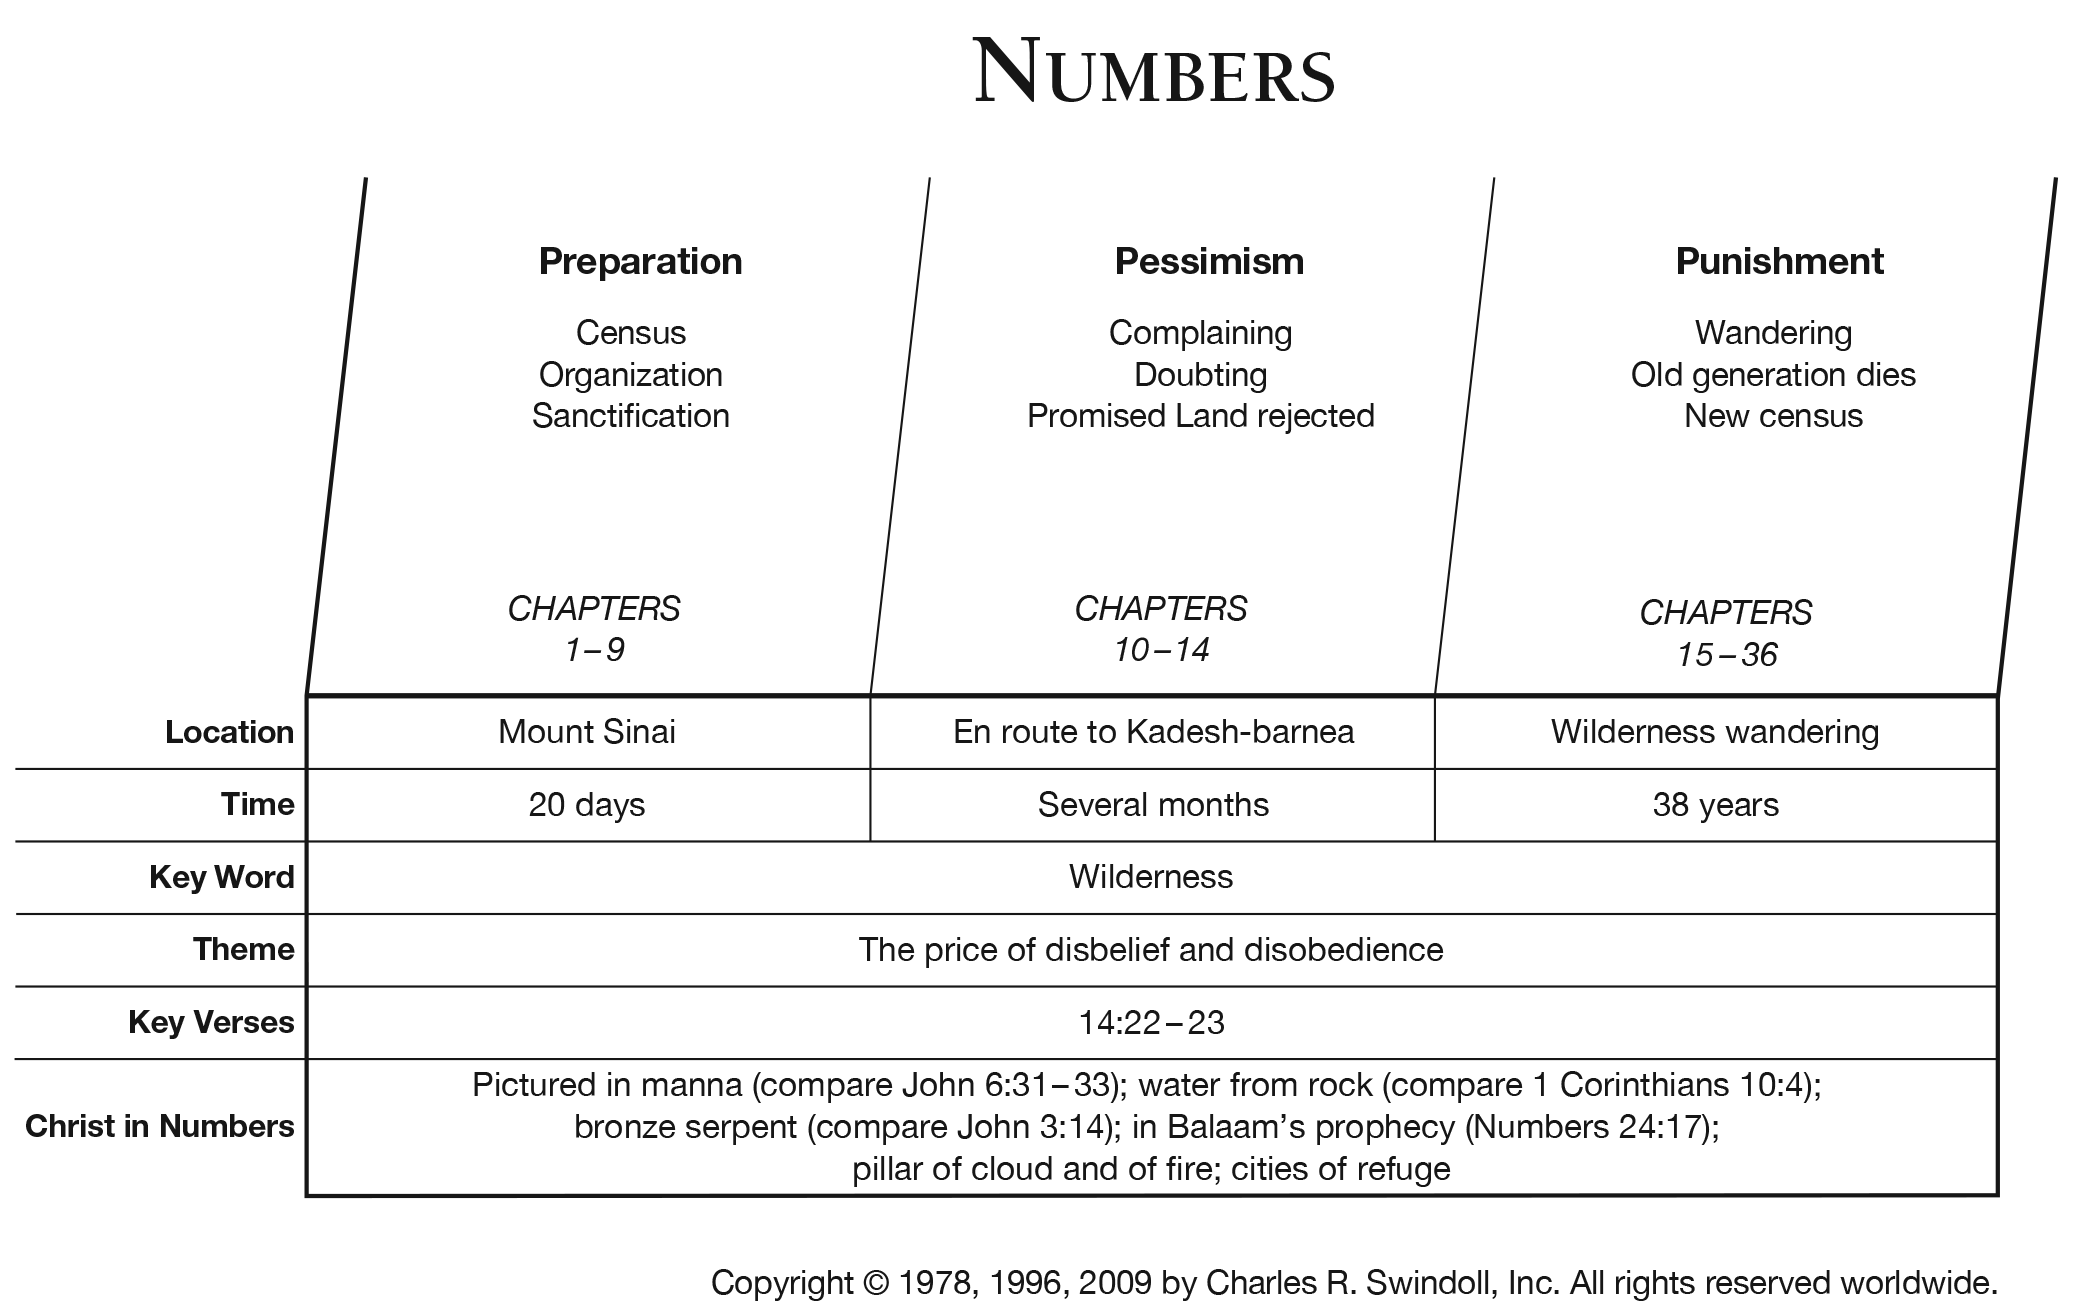
\includegraphics[scale=0.3, angle=90]{04OT-Numbers/References/Swindoll-Numbers.png}
\caption[Numbers by Swindoll]{Numbers by Swindoll}
\label{fig:Numbers by Swindoll}
\end{center}
\end{figure}

\newpage
\begin{figure}
\begin{center}
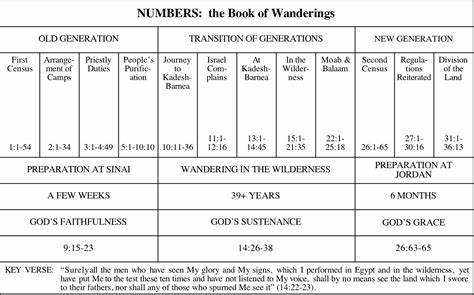
\includegraphics[scale=1.2, angle=90]{04OT-Numbers/References/Numbers.jpg}
\caption[Numbers by Unknown]{Numbers by Unknown}
\label{fig:Numbers by Unknown}
\end{center}
\end{figure}

\newpage
\begin{figure}
\begin{center}
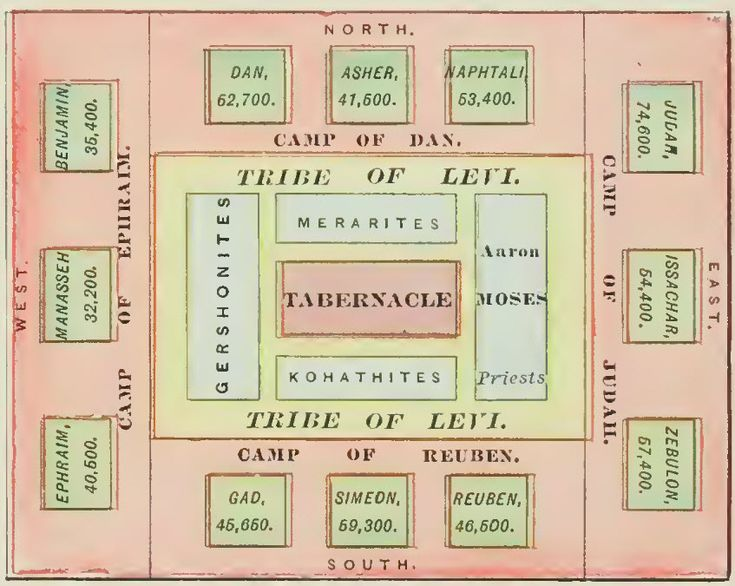
\includegraphics[scale=.8, angle=0]{04OT-Numbers/References/LayoutOfTribesAndTabernacle.jpg}
\caption[Layout of Tribes and Tabernacle]{Layout of Tribes and Tabernacle}
\label{fig:Layout of Tribes and Tabernacle}
\end{center}
\end{figure}


\chapter{Numbers 22}

\begin{figure}
  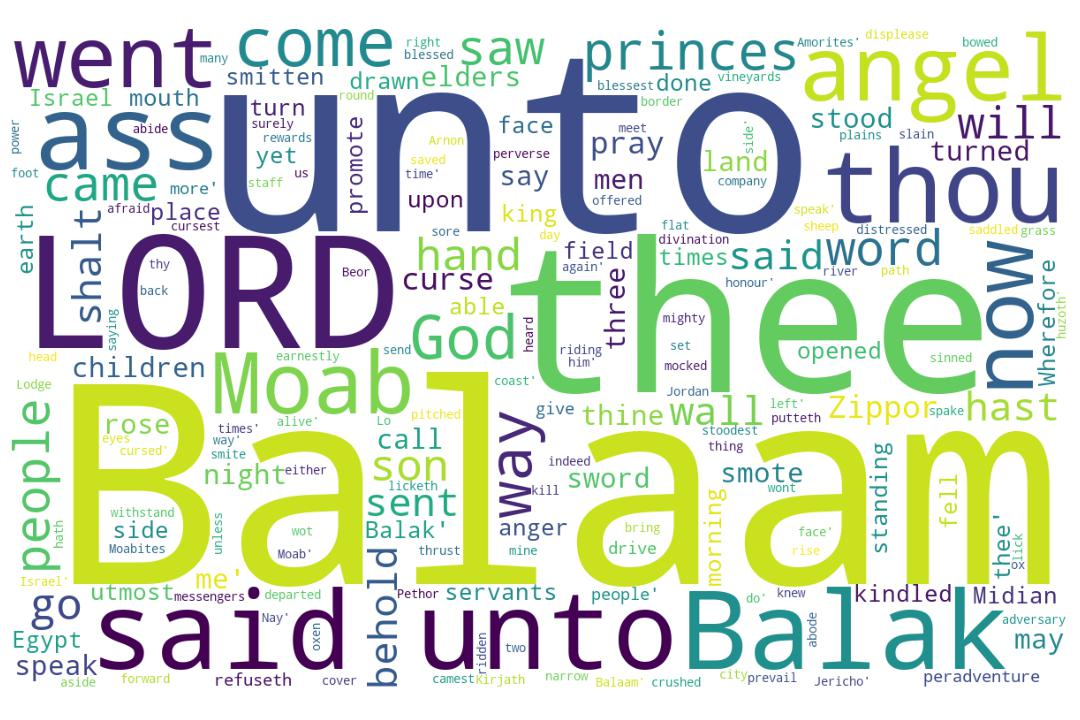
\includegraphics[width=\linewidth]{04OT-Numbers/Numbers22-WordCloud.jpg}
  \caption{Numbers 22 Word Cloud}
  \label{fig:Numbers 22 word Cloud}
\end{figure}

\marginpar{\scriptsize \centering \fcolorbox{bone}{lime}{\textbf{BALAAM'S RELIGION }}\\ (Numbers 22) \begin{compactenum}[I.][8]
    \item  \textbf{Assigned Diplomats} \index[scripture]{Numbers!Num 22:05}\index[scripture]{Numbers!Num 22:15} (Numbers 22:5, 15)
    \item  \textbf{Asking for Divination} \index[scripture]{Numbers!Num 22:07} (Numbers 22:7)
    \item Balaam's \textbf{Attempted Disobedience} \index[scripture]{Numbers!Num 22:19} (Numbers 22:19)
    \item \textbf{Armament Drawn} \index[scripture]{Numbers!Num 22:23}\index[scripture]{Numbers!Num 22:31} (Numbers 22:23, 31)
    \item The \textbf{Ass falls Down} \index[scripture]{Numbers!Num 22:27} (Numbers 22:27)
    \item An \textbf{Argument with a Donkey} \index[scripture]{Numbers!Num 22:29} (Numbers 22:29)
    \item An \textbf{Acquired Doctrine} \index[scripture]{Numbers!Num 23}\index[scripture]{Revelation!Rev 02:14} (Numbers 22, Revelation 2:14)
\end{compactenum}}

%%%%%%%%%%%%%%%%%%%%%%%%%%%%%%%%%%%%%
%%%%%%%%%%%%%%%%%%%%%%%%%%%%%%%%%%%%%
\footnote{\textcolor[rgb]{0.00,0.25,0.00}{\hyperlink{NumbersTOC}{Return to end of Table of Contents.}}}\footnote{\href{https://audiobible.com/bible/numbers_22.html}{\textcolor[cmyk]{0.99998,1,0,0}{Numbers 22 Audio}}}\textcolor[cmyk]{0.99998,1,0,0}{And the children of Israel set forward, and pitched in the plains of Moab on this side Jordan \emph{by} Jericho.}\\
\\
\P \textcolor[cmyk]{0.99998,1,0,0}{And Balak the son of Zippor saw all that Israel had done to the Amorites.}
[3] \textcolor[cmyk]{0.99998,1,0,0}{And Moab was sore afraid of the people, because they \emph{were} many: and Moab was distressed because of the children of Israel.}
[4] \textcolor[cmyk]{0.99998,1,0,0}{And Moab said unto the elders of Midian, Now shall this company lick up all \emph{that} \emph{are} round about us, as the ox licketh up the grass of the field. And Balak the son of Zippor \emph{was} king of the Moabites at that time.}
[5] \textcolor[cmyk]{0.99998,1,0,0}{He sent messengers therefore unto Balaam the son of Beor to Pethor, which \emph{is} by the river of the land of the children of his people, to call him, saying, Behold, there is a people come out from Egypt: behold, they cover the face of the earth, and they abide over against me:}
[6] \textcolor[cmyk]{0.99998,1,0,0}{Come now therefore, I pray thee, curse me this people; for they \emph{are} too mighty for me: peradventure I shall prevail, \emph{that} we may smite them, and \emph{that} I may drive them out of the land: for I wot that he whom thou blessest \emph{is} blessed, and he whom thou cursest is cursed.}
[7] \textcolor[cmyk]{0.99998,1,0,0}{And the elders of Moab and the elders of Midian departed with the rewards of divination in their hand; and they came unto Balaam, and spake unto him the words of Balak.}
[8] \textcolor[cmyk]{0.99998,1,0,0}{And he said unto them, Lodge here this night, and I will bring you word again, as the LORD shall speak unto me: and the princes of Moab abode with Balaam.}
[9] \textcolor[cmyk]{0.99998,1,0,0}{And God came unto Balaam, and said, What men \emph{are} these with thee?}
[10] \textcolor[cmyk]{0.99998,1,0,0}{And Balaam said unto God, Balak the son of Zippor, king of Moab, hath sent unto me, \emph{saying},}
[11] \textcolor[cmyk]{0.99998,1,0,0}{Behold, \emph{there} \emph{is} a people come out of Egypt, which covereth the face of the earth: come now, curse me them; peradventure I shall be able to overcome them, and drive them out.}
[12] \textcolor[cmyk]{0.99998,1,0,0}{And God said unto Balaam, Thou shalt not go with them; thou shalt not curse the people: for they \emph{are} blessed.}
[13] \textcolor[cmyk]{0.99998,1,0,0}{And Balaam rose up in the morning, and said unto the princes of Balak, Get you into your land: for the LORD refuseth to give me leave to go with you.}
[14] \textcolor[cmyk]{0.99998,1,0,0}{And the princes of Moab rose up, and they went unto Balak, and said, Balaam refuseth to come with us.}\\
\\
\P \textcolor[cmyk]{0.99998,1,0,0}{And Balak sent yet again princes, more, and more honourable than they.}
[16] \textcolor[cmyk]{0.99998,1,0,0}{And they came to Balaam, and said to him, Thus saith Balak the son of Zippor, Let nothing, I pray thee, hinder thee from coming unto me:}
[17] \textcolor[cmyk]{0.99998,1,0,0}{For I will promote thee unto very great honour, and I will do whatsoever thou sayest unto me: come therefore, I pray thee, curse me this people.}
[18] \textcolor[cmyk]{0.99998,1,0,0}{And Balaam answered and said unto the servants of Balak, If Balak would give me his house full of silver and gold, I cannot go beyond the word of the LORD my God, to do less or more.}
[19] \textcolor[cmyk]{0.99998,1,0,0}{Now therefore, I pray you, tarry ye also here this night, that I may know what the LORD will say unto me more.}
[20] \textcolor[cmyk]{0.99998,1,0,0}{And God came unto Balaam at night, and said unto him, If the men come to call thee, rise up, \emph{and} go with them; but yet the word which I shall say unto thee, that shalt thou do.}
[21] \textcolor[cmyk]{0.99998,1,0,0}{And Balaam rose up in the morning, and saddled his ass, and went with the princes of Moab.}\\
\\
\P  \textcolor[cmyk]{0.99998,1,0,0}{And God's anger was kindled because he went: and the angel of the LORD stood in the way for an adversary against him. Now he was riding upon his ass, and his two servants \emph{were} with him.}
[23] \textcolor[cmyk]{0.99998,1,0,0}{And the ass saw the angel of the LORD standing in the way, and his sword drawn in his hand: and the ass turned aside out of the way, and went into the field: and Balaam smote the ass, to turn her into the way.}
[24] \textcolor[cmyk]{0.99998,1,0,0}{But the angel of the LORD stood in a path of the vineyards, a wall \emph{being} on this side, and a wall on that side.}
[25] \textcolor[cmyk]{0.99998,1,0,0}{And when the ass saw the angel of the LORD, she thrust herself unto the wall, and crushed Balaam's foot against the wall: and he smote her again.}
[26] \textcolor[cmyk]{0.99998,1,0,0}{And the angel of the LORD went further, and stood in a narrow place, where \emph{was} no way to turn either to the right hand or to the left.}
[27] \textcolor[cmyk]{0.99998,1,0,0}{And when the ass saw the angel of the LORD, she fell down under Balaam: and Balaam's anger was kindled, and he smote the ass with a staff.}
[28] \textcolor[cmyk]{0.99998,1,0,0}{And the LORD opened the mouth of the ass, and she said unto Balaam, What have I done unto thee, that thou hast smitten me these three times?}
[29] \textcolor[cmyk]{0.99998,1,0,0}{And Balaam said unto the ass, Because thou hast mocked me: I would there were a sword in mine hand, for now would I kill thee.}
[30] \textcolor[cmyk]{0.99998,1,0,0}{And the ass said unto Balaam, \emph{Am} not I thine ass, upon which thou hast ridden ever since \emph{I} \emph{was} thine unto this day? was I ever wont to do so unto thee? And he said, Nay.}
[31] \textcolor[cmyk]{0.99998,1,0,0}{Then the LORD opened the eyes of Balaam, and he saw the angel of the LORD standing in the way, and his sword drawn in his hand: and he bowed down his head, and fell flat on his face.}
[32] \textcolor[cmyk]{0.99998,1,0,0}{And the angel of the LORD said unto him, Wherefore hast thou smitten thine ass these three times? behold, I went out to withstand thee, because \emph{thy} way is perverse before me:}
[33] \textcolor[cmyk]{0.99998,1,0,0}{And the ass saw me, and turned from me these three times: unless she had turned from me, surely now also I had slain thee, and saved her alive.}
[34] \textcolor[cmyk]{0.99998,1,0,0}{And Balaam said unto the angel of the LORD, I have sinned; for I knew not that thou stoodest in the way against me: now therefore, if it displease thee, I will get me back again.}
[35] \textcolor[cmyk]{0.99998,1,0,0}{And the angel of the LORD said unto Balaam, Go with the men: but only the word that I shall speak unto thee, that thou shalt speak. So Balaam went with the princes of Balak.}
[36] \textcolor[cmyk]{0.99998,1,0,0}{And when Balak heard that Balaam was come, he went out to meet him unto a city of Moab, which \emph{is} in the border of Arnon, which \emph{is} in the utmost coast.}
[37] \textcolor[cmyk]{0.99998,1,0,0}{And Balak said unto Balaam, Did I not earnestly send unto thee to call thee? wherefore camest thou not unto me? am I not able indeed to promote thee to honour?}
[38] \textcolor[cmyk]{0.99998,1,0,0}{And Balaam said unto Balak, Lo, I am come unto thee: have I now any power at all to say any thing? the word that God putteth in my mouth, that shall I speak.}
[39] \textcolor[cmyk]{0.99998,1,0,0}{And Balaam went with Balak, and they came unto Kirjath-huzoth.}
[40] \textcolor[cmyk]{0.99998,1,0,0}{And Balak offered oxen and sheep, and sent to Balaam, and to the princes that \emph{were} with him.}
[41] \textcolor[cmyk]{0.99998,1,0,0}{And it came to pass on the morrow, that Balak took Balaam, and brought him up into the high places of Baal, that thence he might see the utmost \emph{part} of the people.}
\index[NWIV]{20!Numbers!Num 22:1}\index[AWIP]{And!Numbers!Num 22:1}\index[AWIP]{the!Numbers!Num 22:1}\index[AWIP]{the!Numbers!Num 22:1 (2)}\index[AWIP]{children!Numbers!Num 22:1}\index[AWIP]{of!Numbers!Num 22:1}\index[AWIP]{of!Numbers!Num 22:1 (2)}\index[AWIP]{Israel!Numbers!Num 22:1}\index[AWIP]{set!Numbers!Num 22:1}\index[AWIP]{forward!Numbers!Num 22:1}\index[AWIP]{and!Numbers!Num 22:1}\index[AWIP]{pitched!Numbers!Num 22:1}\index[AWIP]{in!Numbers!Num 22:1}\index[AWIP]{plains!Numbers!Num 22:1}\index[AWIP]{Moab!Numbers!Num 22:1}\index[AWIP]{on!Numbers!Num 22:1}\index[AWIP]{this!Numbers!Num 22:1}\index[AWIP]{side!Numbers!Num 22:1}\index[AWIP]{Jordan!Numbers!Num 22:1}\index[AWIP]{\emph{by}!Numbers!Num 22:1}\index[AWIP]{Jericho!Numbers!Num 22:1}\index[AWIP]{\emph{by}!Numbers!Num 22:1}

\index[NWIV]{15!Numbers!Num 22:2}\index[AWIP]{And!Numbers!Num 22:2}\index[AWIP]{Balak!Numbers!Num 22:2}\index[AWIP]{the!Numbers!Num 22:2}\index[AWIP]{the!Numbers!Num 22:2 (2)}\index[AWIP]{son!Numbers!Num 22:2}\index[AWIP]{of!Numbers!Num 22:2}\index[AWIP]{Zippor!Numbers!Num 22:2}\index[AWIP]{saw!Numbers!Num 22:2}\index[AWIP]{all!Numbers!Num 22:2}\index[AWIP]{that!Numbers!Num 22:2}\index[AWIP]{Israel!Numbers!Num 22:2}\index[AWIP]{had!Numbers!Num 22:2}\index[AWIP]{done!Numbers!Num 22:2}\index[AWIP]{to!Numbers!Num 22:2}\index[AWIP]{Amorites!Numbers!Num 22:2}

\index[NWIV]{22!Numbers!Num 22:3}\index[AWIP]{And!Numbers!Num 22:3}\index[AWIP]{Moab!Numbers!Num 22:3}\index[AWIP]{Moab!Numbers!Num 22:3 (2)}\index[AWIP]{was!Numbers!Num 22:3}\index[AWIP]{was!Numbers!Num 22:3 (2)}\index[AWIP]{sore!Numbers!Num 22:3}\index[AWIP]{afraid!Numbers!Num 22:3}\index[AWIP]{of!Numbers!Num 22:3}\index[AWIP]{of!Numbers!Num 22:3 (2)}\index[AWIP]{of!Numbers!Num 22:3 (3)}\index[AWIP]{the!Numbers!Num 22:3}\index[AWIP]{the!Numbers!Num 22:3 (2)}\index[AWIP]{people!Numbers!Num 22:3}\index[AWIP]{because!Numbers!Num 22:3}\index[AWIP]{because!Numbers!Num 22:3 (2)}\index[AWIP]{they!Numbers!Num 22:3}\index[AWIP]{\emph{were}!Numbers!Num 22:3}\index[AWIP]{many!Numbers!Num 22:3}\index[AWIP]{and!Numbers!Num 22:3}\index[AWIP]{distressed!Numbers!Num 22:3}\index[AWIP]{children!Numbers!Num 22:3}\index[AWIP]{Israel!Numbers!Num 22:3}\index[AWIP]{\emph{were}!Numbers!Num 22:3}

\index[NWIV]{44!Numbers!Num 22:4}\index[AWIP]{And!Numbers!Num 22:4}\index[AWIP]{And!Numbers!Num 22:4 (2)}\index[AWIP]{Moab!Numbers!Num 22:4}\index[AWIP]{said!Numbers!Num 22:4}\index[AWIP]{unto!Numbers!Num 22:4}\index[AWIP]{the!Numbers!Num 22:4}\index[AWIP]{the!Numbers!Num 22:4 (2)}\index[AWIP]{the!Numbers!Num 22:4 (3)}\index[AWIP]{the!Numbers!Num 22:4 (4)}\index[AWIP]{the!Numbers!Num 22:4 (5)}\index[AWIP]{the!Numbers!Num 22:4 (6)}\index[AWIP]{elders!Numbers!Num 22:4}\index[AWIP]{of!Numbers!Num 22:4}\index[AWIP]{of!Numbers!Num 22:4 (2)}\index[AWIP]{of!Numbers!Num 22:4 (3)}\index[AWIP]{of!Numbers!Num 22:4 (4)}\index[AWIP]{Midian!Numbers!Num 22:4}\index[AWIP]{Now!Numbers!Num 22:4}\index[AWIP]{shall!Numbers!Num 22:4}\index[AWIP]{this!Numbers!Num 22:4}\index[AWIP]{company!Numbers!Num 22:4}\index[AWIP]{lick!Numbers!Num 22:4}\index[AWIP]{up!Numbers!Num 22:4}\index[AWIP]{up!Numbers!Num 22:4 (2)}\index[AWIP]{all!Numbers!Num 22:4}\index[AWIP]{\emph{that}!Numbers!Num 22:4}\index[AWIP]{\emph{are}!Numbers!Num 22:4}\index[AWIP]{round!Numbers!Num 22:4}\index[AWIP]{about!Numbers!Num 22:4}\index[AWIP]{us!Numbers!Num 22:4}\index[AWIP]{as!Numbers!Num 22:4}\index[AWIP]{ox!Numbers!Num 22:4}\index[AWIP]{licketh!Numbers!Num 22:4}\index[AWIP]{grass!Numbers!Num 22:4}\index[AWIP]{field!Numbers!Num 22:4}\index[AWIP]{Balak!Numbers!Num 22:4}\index[AWIP]{son!Numbers!Num 22:4}\index[AWIP]{Zippor!Numbers!Num 22:4}\index[AWIP]{\emph{was}!Numbers!Num 22:4}\index[AWIP]{king!Numbers!Num 22:4}\index[AWIP]{Moabites!Numbers!Num 22:4}\index[AWIP]{at!Numbers!Num 22:4}\index[AWIP]{that!Numbers!Num 22:4}\index[AWIP]{time!Numbers!Num 22:4}\index[AWIP]{\emph{that}!Numbers!Num 22:4}\index[AWIP]{\emph{are}!Numbers!Num 22:4}\index[AWIP]{\emph{was}!Numbers!Num 22:4}

\index[NWIV]{53!Numbers!Num 22:5}\index[AWIP]{He!Numbers!Num 22:5}\index[AWIP]{sent!Numbers!Num 22:5}\index[AWIP]{messengers!Numbers!Num 22:5}\index[AWIP]{therefore!Numbers!Num 22:5}\index[AWIP]{unto!Numbers!Num 22:5}\index[AWIP]{Balaam!Numbers!Num 22:5}\index[AWIP]{the!Numbers!Num 22:5}\index[AWIP]{the!Numbers!Num 22:5 (2)}\index[AWIP]{the!Numbers!Num 22:5 (3)}\index[AWIP]{the!Numbers!Num 22:5 (4)}\index[AWIP]{the!Numbers!Num 22:5 (5)}\index[AWIP]{the!Numbers!Num 22:5 (6)}\index[AWIP]{son!Numbers!Num 22:5}\index[AWIP]{of!Numbers!Num 22:5}\index[AWIP]{of!Numbers!Num 22:5 (2)}\index[AWIP]{of!Numbers!Num 22:5 (3)}\index[AWIP]{of!Numbers!Num 22:5 (4)}\index[AWIP]{of!Numbers!Num 22:5 (5)}\index[AWIP]{Beor!Numbers!Num 22:5}\index[AWIP]{to!Numbers!Num 22:5}\index[AWIP]{to!Numbers!Num 22:5 (2)}\index[AWIP]{Pethor!Numbers!Num 22:5}\index[AWIP]{which!Numbers!Num 22:5}\index[AWIP]{\emph{is}!Numbers!Num 22:5}\index[AWIP]{by!Numbers!Num 22:5}\index[AWIP]{river!Numbers!Num 22:5}\index[AWIP]{land!Numbers!Num 22:5}\index[AWIP]{children!Numbers!Num 22:5}\index[AWIP]{his!Numbers!Num 22:5}\index[AWIP]{people!Numbers!Num 22:5}\index[AWIP]{people!Numbers!Num 22:5 (2)}\index[AWIP]{call!Numbers!Num 22:5}\index[AWIP]{him!Numbers!Num 22:5}\index[AWIP]{saying!Numbers!Num 22:5}\index[AWIP]{Behold!Numbers!Num 22:5}\index[AWIP]{there!Numbers!Num 22:5}\index[AWIP]{is!Numbers!Num 22:5}\index[AWIP]{a!Numbers!Num 22:5}\index[AWIP]{come!Numbers!Num 22:5}\index[AWIP]{out!Numbers!Num 22:5}\index[AWIP]{from!Numbers!Num 22:5}\index[AWIP]{Egypt!Numbers!Num 22:5}\index[AWIP]{behold!Numbers!Num 22:5}\index[AWIP]{they!Numbers!Num 22:5}\index[AWIP]{they!Numbers!Num 22:5 (2)}\index[AWIP]{cover!Numbers!Num 22:5}\index[AWIP]{face!Numbers!Num 22:5}\index[AWIP]{earth!Numbers!Num 22:5}\index[AWIP]{and!Numbers!Num 22:5}\index[AWIP]{abide!Numbers!Num 22:5}\index[AWIP]{over!Numbers!Num 22:5}\index[AWIP]{against!Numbers!Num 22:5}\index[AWIP]{me!Numbers!Num 22:5}\index[AWIP]{\emph{is}!Numbers!Num 22:5}

\index[NWIV]{53!Numbers!Num 22:6}\index[AWIP]{Come!Numbers!Num 22:6}\index[AWIP]{now!Numbers!Num 22:6}\index[AWIP]{therefore!Numbers!Num 22:6}\index[AWIP]{I!Numbers!Num 22:6}\index[AWIP]{I!Numbers!Num 22:6 (2)}\index[AWIP]{I!Numbers!Num 22:6 (3)}\index[AWIP]{I!Numbers!Num 22:6 (4)}\index[AWIP]{pray!Numbers!Num 22:6}\index[AWIP]{thee!Numbers!Num 22:6}\index[AWIP]{curse!Numbers!Num 22:6}\index[AWIP]{me!Numbers!Num 22:6}\index[AWIP]{me!Numbers!Num 22:6 (2)}\index[AWIP]{this!Numbers!Num 22:6}\index[AWIP]{people!Numbers!Num 22:6}\index[AWIP]{for!Numbers!Num 22:6}\index[AWIP]{for!Numbers!Num 22:6 (2)}\index[AWIP]{for!Numbers!Num 22:6 (3)}\index[AWIP]{they!Numbers!Num 22:6}\index[AWIP]{\emph{are}!Numbers!Num 22:6}\index[AWIP]{too!Numbers!Num 22:6}\index[AWIP]{mighty!Numbers!Num 22:6}\index[AWIP]{peradventure!Numbers!Num 22:6}\index[AWIP]{shall!Numbers!Num 22:6}\index[AWIP]{prevail!Numbers!Num 22:6}\index[AWIP]{\emph{that}!Numbers!Num 22:6}\index[AWIP]{\emph{that}!Numbers!Num 22:6 (2)}\index[AWIP]{we!Numbers!Num 22:6}\index[AWIP]{may!Numbers!Num 22:6}\index[AWIP]{may!Numbers!Num 22:6 (2)}\index[AWIP]{smite!Numbers!Num 22:6}\index[AWIP]{them!Numbers!Num 22:6}\index[AWIP]{them!Numbers!Num 22:6 (2)}\index[AWIP]{and!Numbers!Num 22:6}\index[AWIP]{and!Numbers!Num 22:6 (2)}\index[AWIP]{drive!Numbers!Num 22:6}\index[AWIP]{out!Numbers!Num 22:6}\index[AWIP]{of!Numbers!Num 22:6}\index[AWIP]{the!Numbers!Num 22:6}\index[AWIP]{land!Numbers!Num 22:6}\index[AWIP]{wot!Numbers!Num 22:6}\index[AWIP]{that!Numbers!Num 22:6}\index[AWIP]{he!Numbers!Num 22:6}\index[AWIP]{he!Numbers!Num 22:6 (2)}\index[AWIP]{whom!Numbers!Num 22:6}\index[AWIP]{whom!Numbers!Num 22:6 (2)}\index[AWIP]{thou!Numbers!Num 22:6}\index[AWIP]{thou!Numbers!Num 22:6 (2)}\index[AWIP]{blessest!Numbers!Num 22:6}\index[AWIP]{\emph{is}!Numbers!Num 22:6}\index[AWIP]{blessed!Numbers!Num 22:6}\index[AWIP]{cursest!Numbers!Num 22:6}\index[AWIP]{is!Numbers!Num 22:6}\index[AWIP]{cursed!Numbers!Num 22:6}\index[AWIP]{\emph{are}!Numbers!Num 22:6}\index[AWIP]{\emph{that}!Numbers!Num 22:6}\index[AWIP]{\emph{that}!Numbers!Num 22:6 (2)}\index[AWIP]{\emph{is}!Numbers!Num 22:6}

\index[NWIV]{32!Numbers!Num 22:7}\index[AWIP]{And!Numbers!Num 22:7}\index[AWIP]{the!Numbers!Num 22:7}\index[AWIP]{the!Numbers!Num 22:7 (2)}\index[AWIP]{the!Numbers!Num 22:7 (3)}\index[AWIP]{the!Numbers!Num 22:7 (4)}\index[AWIP]{elders!Numbers!Num 22:7}\index[AWIP]{elders!Numbers!Num 22:7 (2)}\index[AWIP]{of!Numbers!Num 22:7}\index[AWIP]{of!Numbers!Num 22:7 (2)}\index[AWIP]{of!Numbers!Num 22:7 (3)}\index[AWIP]{of!Numbers!Num 22:7 (4)}\index[AWIP]{Moab!Numbers!Num 22:7}\index[AWIP]{and!Numbers!Num 22:7}\index[AWIP]{and!Numbers!Num 22:7 (2)}\index[AWIP]{and!Numbers!Num 22:7 (3)}\index[AWIP]{Midian!Numbers!Num 22:7}\index[AWIP]{departed!Numbers!Num 22:7}\index[AWIP]{with!Numbers!Num 22:7}\index[AWIP]{rewards!Numbers!Num 22:7}\index[AWIP]{divination!Numbers!Num 22:7}\index[AWIP]{in!Numbers!Num 22:7}\index[AWIP]{their!Numbers!Num 22:7}\index[AWIP]{hand!Numbers!Num 22:7}\index[AWIP]{they!Numbers!Num 22:7}\index[AWIP]{came!Numbers!Num 22:7}\index[AWIP]{unto!Numbers!Num 22:7}\index[AWIP]{unto!Numbers!Num 22:7 (2)}\index[AWIP]{Balaam!Numbers!Num 22:7}\index[AWIP]{spake!Numbers!Num 22:7}\index[AWIP]{him!Numbers!Num 22:7}\index[AWIP]{words!Numbers!Num 22:7}\index[AWIP]{Balak!Numbers!Num 22:7}

\index[NWIV]{31!Numbers!Num 22:8}\index[AWIP]{And!Numbers!Num 22:8}\index[AWIP]{he!Numbers!Num 22:8}\index[AWIP]{said!Numbers!Num 22:8}\index[AWIP]{unto!Numbers!Num 22:8}\index[AWIP]{unto!Numbers!Num 22:8 (2)}\index[AWIP]{them!Numbers!Num 22:8}\index[AWIP]{Lodge!Numbers!Num 22:8}\index[AWIP]{here!Numbers!Num 22:8}\index[AWIP]{this!Numbers!Num 22:8}\index[AWIP]{night!Numbers!Num 22:8}\index[AWIP]{and!Numbers!Num 22:8}\index[AWIP]{and!Numbers!Num 22:8 (2)}\index[AWIP]{I!Numbers!Num 22:8}\index[AWIP]{will!Numbers!Num 22:8}\index[AWIP]{bring!Numbers!Num 22:8}\index[AWIP]{you!Numbers!Num 22:8}\index[AWIP]{word!Numbers!Num 22:8}\index[AWIP]{again!Numbers!Num 22:8}\index[AWIP]{as!Numbers!Num 22:8}\index[AWIP]{the!Numbers!Num 22:8}\index[AWIP]{the!Numbers!Num 22:8 (2)}\index[AWIP]{LORD!Numbers!Num 22:8}\index[AWIP]{shall!Numbers!Num 22:8}\index[AWIP]{speak!Numbers!Num 22:8}\index[AWIP]{me!Numbers!Num 22:8}\index[AWIP]{princes!Numbers!Num 22:8}\index[AWIP]{of!Numbers!Num 22:8}\index[AWIP]{Moab!Numbers!Num 22:8}\index[AWIP]{abode!Numbers!Num 22:8}\index[AWIP]{with!Numbers!Num 22:8}\index[AWIP]{Balaam!Numbers!Num 22:8}

\index[NWIV]{13!Numbers!Num 22:9}\index[AWIP]{And!Numbers!Num 22:9}\index[AWIP]{God!Numbers!Num 22:9}\index[AWIP]{came!Numbers!Num 22:9}\index[AWIP]{unto!Numbers!Num 22:9}\index[AWIP]{Balaam!Numbers!Num 22:9}\index[AWIP]{and!Numbers!Num 22:9}\index[AWIP]{said!Numbers!Num 22:9}\index[AWIP]{What!Numbers!Num 22:9}\index[AWIP]{men!Numbers!Num 22:9}\index[AWIP]{\emph{are}!Numbers!Num 22:9}\index[AWIP]{these!Numbers!Num 22:9}\index[AWIP]{with!Numbers!Num 22:9}\index[AWIP]{thee?!Numbers!Num 22:9}\index[AWIP]{\emph{are}!Numbers!Num 22:9}

\index[NWIV]{18!Numbers!Num 22:10}\index[AWIP]{And!Numbers!Num 22:10}\index[AWIP]{Balaam!Numbers!Num 22:10}\index[AWIP]{said!Numbers!Num 22:10}\index[AWIP]{unto!Numbers!Num 22:10}\index[AWIP]{unto!Numbers!Num 22:10 (2)}\index[AWIP]{God!Numbers!Num 22:10}\index[AWIP]{Balak!Numbers!Num 22:10}\index[AWIP]{the!Numbers!Num 22:10}\index[AWIP]{son!Numbers!Num 22:10}\index[AWIP]{of!Numbers!Num 22:10}\index[AWIP]{of!Numbers!Num 22:10 (2)}\index[AWIP]{Zippor!Numbers!Num 22:10}\index[AWIP]{king!Numbers!Num 22:10}\index[AWIP]{Moab!Numbers!Num 22:10}\index[AWIP]{hath!Numbers!Num 22:10}\index[AWIP]{sent!Numbers!Num 22:10}\index[AWIP]{me!Numbers!Num 22:10}\index[AWIP]{\emph{saying}!Numbers!Num 22:10}\index[AWIP]{\emph{saying}!Numbers!Num 22:10}

\index[NWIV]{33!Numbers!Num 22:11}\index[AWIP]{Behold!Numbers!Num 22:11}\index[AWIP]{\emph{there}!Numbers!Num 22:11}\index[AWIP]{\emph{is}!Numbers!Num 22:11}\index[AWIP]{a!Numbers!Num 22:11}\index[AWIP]{people!Numbers!Num 22:11}\index[AWIP]{come!Numbers!Num 22:11}\index[AWIP]{come!Numbers!Num 22:11 (2)}\index[AWIP]{out!Numbers!Num 22:11}\index[AWIP]{out!Numbers!Num 22:11 (2)}\index[AWIP]{of!Numbers!Num 22:11}\index[AWIP]{of!Numbers!Num 22:11 (2)}\index[AWIP]{Egypt!Numbers!Num 22:11}\index[AWIP]{which!Numbers!Num 22:11}\index[AWIP]{covereth!Numbers!Num 22:11}\index[AWIP]{the!Numbers!Num 22:11}\index[AWIP]{the!Numbers!Num 22:11 (2)}\index[AWIP]{face!Numbers!Num 22:11}\index[AWIP]{earth!Numbers!Num 22:11}\index[AWIP]{now!Numbers!Num 22:11}\index[AWIP]{curse!Numbers!Num 22:11}\index[AWIP]{me!Numbers!Num 22:11}\index[AWIP]{them!Numbers!Num 22:11}\index[AWIP]{them!Numbers!Num 22:11 (2)}\index[AWIP]{them!Numbers!Num 22:11 (3)}\index[AWIP]{peradventure!Numbers!Num 22:11}\index[AWIP]{I!Numbers!Num 22:11}\index[AWIP]{shall!Numbers!Num 22:11}\index[AWIP]{be!Numbers!Num 22:11}\index[AWIP]{able!Numbers!Num 22:11}\index[AWIP]{to!Numbers!Num 22:11}\index[AWIP]{overcome!Numbers!Num 22:11}\index[AWIP]{and!Numbers!Num 22:11}\index[AWIP]{drive!Numbers!Num 22:11}\index[AWIP]{\emph{there}!Numbers!Num 22:11}\index[AWIP]{\emph{is}!Numbers!Num 22:11}

\index[NWIV]{21!Numbers!Num 22:12}\index[AWIP]{And!Numbers!Num 22:12}\index[AWIP]{God!Numbers!Num 22:12}\index[AWIP]{said!Numbers!Num 22:12}\index[AWIP]{unto!Numbers!Num 22:12}\index[AWIP]{Balaam!Numbers!Num 22:12}\index[AWIP]{Thou!Numbers!Num 22:12}\index[AWIP]{shalt!Numbers!Num 22:12}\index[AWIP]{shalt!Numbers!Num 22:12 (2)}\index[AWIP]{not!Numbers!Num 22:12}\index[AWIP]{not!Numbers!Num 22:12 (2)}\index[AWIP]{go!Numbers!Num 22:12}\index[AWIP]{with!Numbers!Num 22:12}\index[AWIP]{them!Numbers!Num 22:12}\index[AWIP]{thou!Numbers!Num 22:12}\index[AWIP]{curse!Numbers!Num 22:12}\index[AWIP]{the!Numbers!Num 22:12}\index[AWIP]{people!Numbers!Num 22:12}\index[AWIP]{for!Numbers!Num 22:12}\index[AWIP]{they!Numbers!Num 22:12}\index[AWIP]{\emph{are}!Numbers!Num 22:12}\index[AWIP]{blessed!Numbers!Num 22:12}\index[AWIP]{\emph{are}!Numbers!Num 22:12}

\index[NWIV]{31!Numbers!Num 22:13}\index[AWIP]{And!Numbers!Num 22:13}\index[AWIP]{Balaam!Numbers!Num 22:13}\index[AWIP]{rose!Numbers!Num 22:13}\index[AWIP]{up!Numbers!Num 22:13}\index[AWIP]{in!Numbers!Num 22:13}\index[AWIP]{the!Numbers!Num 22:13}\index[AWIP]{the!Numbers!Num 22:13 (2)}\index[AWIP]{the!Numbers!Num 22:13 (3)}\index[AWIP]{morning!Numbers!Num 22:13}\index[AWIP]{and!Numbers!Num 22:13}\index[AWIP]{said!Numbers!Num 22:13}\index[AWIP]{unto!Numbers!Num 22:13}\index[AWIP]{princes!Numbers!Num 22:13}\index[AWIP]{of!Numbers!Num 22:13}\index[AWIP]{Balak!Numbers!Num 22:13}\index[AWIP]{Get!Numbers!Num 22:13}\index[AWIP]{you!Numbers!Num 22:13}\index[AWIP]{you!Numbers!Num 22:13 (2)}\index[AWIP]{into!Numbers!Num 22:13}\index[AWIP]{your!Numbers!Num 22:13}\index[AWIP]{land!Numbers!Num 22:13}\index[AWIP]{for!Numbers!Num 22:13}\index[AWIP]{LORD!Numbers!Num 22:13}\index[AWIP]{refuseth!Numbers!Num 22:13}\index[AWIP]{to!Numbers!Num 22:13}\index[AWIP]{to!Numbers!Num 22:13 (2)}\index[AWIP]{give!Numbers!Num 22:13}\index[AWIP]{me!Numbers!Num 22:13}\index[AWIP]{leave!Numbers!Num 22:13}\index[AWIP]{go!Numbers!Num 22:13}\index[AWIP]{with!Numbers!Num 22:13}

\index[NWIV]{20!Numbers!Num 22:14}\index[AWIP]{And!Numbers!Num 22:14}\index[AWIP]{the!Numbers!Num 22:14}\index[AWIP]{princes!Numbers!Num 22:14}\index[AWIP]{of!Numbers!Num 22:14}\index[AWIP]{Moab!Numbers!Num 22:14}\index[AWIP]{rose!Numbers!Num 22:14}\index[AWIP]{up!Numbers!Num 22:14}\index[AWIP]{and!Numbers!Num 22:14}\index[AWIP]{and!Numbers!Num 22:14 (2)}\index[AWIP]{they!Numbers!Num 22:14}\index[AWIP]{went!Numbers!Num 22:14}\index[AWIP]{unto!Numbers!Num 22:14}\index[AWIP]{Balak!Numbers!Num 22:14}\index[AWIP]{said!Numbers!Num 22:14}\index[AWIP]{Balaam!Numbers!Num 22:14}\index[AWIP]{refuseth!Numbers!Num 22:14}\index[AWIP]{to!Numbers!Num 22:14}\index[AWIP]{come!Numbers!Num 22:14}\index[AWIP]{with!Numbers!Num 22:14}\index[AWIP]{us!Numbers!Num 22:14}

\index[NWIV]{12!Numbers!Num 22:15}\index[AWIP]{And!Numbers!Num 22:15}\index[AWIP]{Balak!Numbers!Num 22:15}\index[AWIP]{sent!Numbers!Num 22:15}\index[AWIP]{yet!Numbers!Num 22:15}\index[AWIP]{again!Numbers!Num 22:15}\index[AWIP]{princes!Numbers!Num 22:15}\index[AWIP]{more!Numbers!Num 22:15}\index[AWIP]{more!Numbers!Num 22:15 (2)}\index[AWIP]{and!Numbers!Num 22:15}\index[AWIP]{honourable!Numbers!Num 22:15}\index[AWIP]{than!Numbers!Num 22:15}\index[AWIP]{they!Numbers!Num 22:15}

\index[NWIV]{27!Numbers!Num 22:16}\index[AWIP]{And!Numbers!Num 22:16}\index[AWIP]{they!Numbers!Num 22:16}\index[AWIP]{came!Numbers!Num 22:16}\index[AWIP]{to!Numbers!Num 22:16}\index[AWIP]{to!Numbers!Num 22:16 (2)}\index[AWIP]{Balaam!Numbers!Num 22:16}\index[AWIP]{and!Numbers!Num 22:16}\index[AWIP]{said!Numbers!Num 22:16}\index[AWIP]{him!Numbers!Num 22:16}\index[AWIP]{Thus!Numbers!Num 22:16}\index[AWIP]{saith!Numbers!Num 22:16}\index[AWIP]{Balak!Numbers!Num 22:16}\index[AWIP]{the!Numbers!Num 22:16}\index[AWIP]{son!Numbers!Num 22:16}\index[AWIP]{of!Numbers!Num 22:16}\index[AWIP]{Zippor!Numbers!Num 22:16}\index[AWIP]{Let!Numbers!Num 22:16}\index[AWIP]{nothing!Numbers!Num 22:16}\index[AWIP]{I!Numbers!Num 22:16}\index[AWIP]{pray!Numbers!Num 22:16}\index[AWIP]{thee!Numbers!Num 22:16}\index[AWIP]{thee!Numbers!Num 22:16 (2)}\index[AWIP]{hinder!Numbers!Num 22:16}\index[AWIP]{from!Numbers!Num 22:16}\index[AWIP]{coming!Numbers!Num 22:16}\index[AWIP]{unto!Numbers!Num 22:16}\index[AWIP]{me!Numbers!Num 22:16}

\index[NWIV]{27!Numbers!Num 22:17}\index[AWIP]{For!Numbers!Num 22:17}\index[AWIP]{I!Numbers!Num 22:17}\index[AWIP]{I!Numbers!Num 22:17 (2)}\index[AWIP]{I!Numbers!Num 22:17 (3)}\index[AWIP]{will!Numbers!Num 22:17}\index[AWIP]{will!Numbers!Num 22:17 (2)}\index[AWIP]{promote!Numbers!Num 22:17}\index[AWIP]{thee!Numbers!Num 22:17}\index[AWIP]{thee!Numbers!Num 22:17 (2)}\index[AWIP]{unto!Numbers!Num 22:17}\index[AWIP]{unto!Numbers!Num 22:17 (2)}\index[AWIP]{very!Numbers!Num 22:17}\index[AWIP]{great!Numbers!Num 22:17}\index[AWIP]{honour!Numbers!Num 22:17}\index[AWIP]{and!Numbers!Num 22:17}\index[AWIP]{do!Numbers!Num 22:17}\index[AWIP]{whatsoever!Numbers!Num 22:17}\index[AWIP]{thou!Numbers!Num 22:17}\index[AWIP]{sayest!Numbers!Num 22:17}\index[AWIP]{me!Numbers!Num 22:17}\index[AWIP]{me!Numbers!Num 22:17 (2)}\index[AWIP]{come!Numbers!Num 22:17}\index[AWIP]{therefore!Numbers!Num 22:17}\index[AWIP]{pray!Numbers!Num 22:17}\index[AWIP]{curse!Numbers!Num 22:17}\index[AWIP]{this!Numbers!Num 22:17}\index[AWIP]{people!Numbers!Num 22:17}

\index[NWIV]{38!Numbers!Num 22:18}\index[AWIP]{And!Numbers!Num 22:18}\index[AWIP]{Balaam!Numbers!Num 22:18}\index[AWIP]{answered!Numbers!Num 22:18}\index[AWIP]{and!Numbers!Num 22:18}\index[AWIP]{and!Numbers!Num 22:18 (2)}\index[AWIP]{said!Numbers!Num 22:18}\index[AWIP]{unto!Numbers!Num 22:18}\index[AWIP]{the!Numbers!Num 22:18}\index[AWIP]{the!Numbers!Num 22:18 (2)}\index[AWIP]{the!Numbers!Num 22:18 (3)}\index[AWIP]{servants!Numbers!Num 22:18}\index[AWIP]{of!Numbers!Num 22:18}\index[AWIP]{of!Numbers!Num 22:18 (2)}\index[AWIP]{of!Numbers!Num 22:18 (3)}\index[AWIP]{Balak!Numbers!Num 22:18}\index[AWIP]{Balak!Numbers!Num 22:18 (2)}\index[AWIP]{If!Numbers!Num 22:18}\index[AWIP]{would!Numbers!Num 22:18}\index[AWIP]{give!Numbers!Num 22:18}\index[AWIP]{me!Numbers!Num 22:18}\index[AWIP]{his!Numbers!Num 22:18}\index[AWIP]{house!Numbers!Num 22:18}\index[AWIP]{full!Numbers!Num 22:18}\index[AWIP]{silver!Numbers!Num 22:18}\index[AWIP]{gold!Numbers!Num 22:18}\index[AWIP]{I!Numbers!Num 22:18}\index[AWIP]{cannot!Numbers!Num 22:18}\index[AWIP]{go!Numbers!Num 22:18}\index[AWIP]{beyond!Numbers!Num 22:18}\index[AWIP]{word!Numbers!Num 22:18}\index[AWIP]{LORD!Numbers!Num 22:18}\index[AWIP]{my!Numbers!Num 22:18}\index[AWIP]{God!Numbers!Num 22:18}\index[AWIP]{to!Numbers!Num 22:18}\index[AWIP]{do!Numbers!Num 22:18}\index[AWIP]{less!Numbers!Num 22:18}\index[AWIP]{or!Numbers!Num 22:18}\index[AWIP]{more!Numbers!Num 22:18}

\index[NWIV]{23!Numbers!Num 22:19}\index[AWIP]{Now!Numbers!Num 22:19}\index[AWIP]{therefore!Numbers!Num 22:19}\index[AWIP]{I!Numbers!Num 22:19}\index[AWIP]{I!Numbers!Num 22:19 (2)}\index[AWIP]{pray!Numbers!Num 22:19}\index[AWIP]{you!Numbers!Num 22:19}\index[AWIP]{tarry!Numbers!Num 22:19}\index[AWIP]{ye!Numbers!Num 22:19}\index[AWIP]{also!Numbers!Num 22:19}\index[AWIP]{here!Numbers!Num 22:19}\index[AWIP]{this!Numbers!Num 22:19}\index[AWIP]{night!Numbers!Num 22:19}\index[AWIP]{that!Numbers!Num 22:19}\index[AWIP]{may!Numbers!Num 22:19}\index[AWIP]{know!Numbers!Num 22:19}\index[AWIP]{what!Numbers!Num 22:19}\index[AWIP]{the!Numbers!Num 22:19}\index[AWIP]{LORD!Numbers!Num 22:19}\index[AWIP]{will!Numbers!Num 22:19}\index[AWIP]{say!Numbers!Num 22:19}\index[AWIP]{unto!Numbers!Num 22:19}\index[AWIP]{me!Numbers!Num 22:19}\index[AWIP]{more!Numbers!Num 22:19}

\index[NWIV]{38!Numbers!Num 22:20}\index[AWIP]{And!Numbers!Num 22:20}\index[AWIP]{God!Numbers!Num 22:20}\index[AWIP]{came!Numbers!Num 22:20}\index[AWIP]{unto!Numbers!Num 22:20}\index[AWIP]{unto!Numbers!Num 22:20 (2)}\index[AWIP]{unto!Numbers!Num 22:20 (3)}\index[AWIP]{Balaam!Numbers!Num 22:20}\index[AWIP]{at!Numbers!Num 22:20}\index[AWIP]{night!Numbers!Num 22:20}\index[AWIP]{and!Numbers!Num 22:20}\index[AWIP]{said!Numbers!Num 22:20}\index[AWIP]{him!Numbers!Num 22:20}\index[AWIP]{If!Numbers!Num 22:20}\index[AWIP]{the!Numbers!Num 22:20}\index[AWIP]{the!Numbers!Num 22:20 (2)}\index[AWIP]{men!Numbers!Num 22:20}\index[AWIP]{come!Numbers!Num 22:20}\index[AWIP]{to!Numbers!Num 22:20}\index[AWIP]{call!Numbers!Num 22:20}\index[AWIP]{thee!Numbers!Num 22:20}\index[AWIP]{thee!Numbers!Num 22:20 (2)}\index[AWIP]{rise!Numbers!Num 22:20}\index[AWIP]{up!Numbers!Num 22:20}\index[AWIP]{\emph{and}!Numbers!Num 22:20}\index[AWIP]{go!Numbers!Num 22:20}\index[AWIP]{with!Numbers!Num 22:20}\index[AWIP]{them!Numbers!Num 22:20}\index[AWIP]{but!Numbers!Num 22:20}\index[AWIP]{yet!Numbers!Num 22:20}\index[AWIP]{word!Numbers!Num 22:20}\index[AWIP]{which!Numbers!Num 22:20}\index[AWIP]{I!Numbers!Num 22:20}\index[AWIP]{shall!Numbers!Num 22:20}\index[AWIP]{say!Numbers!Num 22:20}\index[AWIP]{that!Numbers!Num 22:20}\index[AWIP]{shalt!Numbers!Num 22:20}\index[AWIP]{thou!Numbers!Num 22:20}\index[AWIP]{do!Numbers!Num 22:20}\index[AWIP]{\emph{and}!Numbers!Num 22:20}

\index[NWIV]{18!Numbers!Num 22:21}\index[AWIP]{And!Numbers!Num 22:21}\index[AWIP]{Balaam!Numbers!Num 22:21}\index[AWIP]{rose!Numbers!Num 22:21}\index[AWIP]{up!Numbers!Num 22:21}\index[AWIP]{in!Numbers!Num 22:21}\index[AWIP]{the!Numbers!Num 22:21}\index[AWIP]{the!Numbers!Num 22:21 (2)}\index[AWIP]{morning!Numbers!Num 22:21}\index[AWIP]{and!Numbers!Num 22:21}\index[AWIP]{and!Numbers!Num 22:21 (2)}\index[AWIP]{saddled!Numbers!Num 22:21}\index[AWIP]{his!Numbers!Num 22:21}\index[AWIP]{ass!Numbers!Num 22:21}\index[AWIP]{went!Numbers!Num 22:21}\index[AWIP]{with!Numbers!Num 22:21}\index[AWIP]{princes!Numbers!Num 22:21}\index[AWIP]{of!Numbers!Num 22:21}\index[AWIP]{Moab!Numbers!Num 22:21}

\index[NWIV]{37!Numbers!Num 22:22}\index[AWIP]{And!Numbers!Num 22:22}\index[AWIP]{God's!Numbers!Num 22:22}\index[AWIP]{anger!Numbers!Num 22:22}\index[AWIP]{was!Numbers!Num 22:22}\index[AWIP]{was!Numbers!Num 22:22 (2)}\index[AWIP]{kindled!Numbers!Num 22:22}\index[AWIP]{because!Numbers!Num 22:22}\index[AWIP]{he!Numbers!Num 22:22}\index[AWIP]{he!Numbers!Num 22:22 (2)}\index[AWIP]{went!Numbers!Num 22:22}\index[AWIP]{and!Numbers!Num 22:22}\index[AWIP]{and!Numbers!Num 22:22 (2)}\index[AWIP]{the!Numbers!Num 22:22}\index[AWIP]{the!Numbers!Num 22:22 (2)}\index[AWIP]{the!Numbers!Num 22:22 (3)}\index[AWIP]{angel!Numbers!Num 22:22}\index[AWIP]{of!Numbers!Num 22:22}\index[AWIP]{LORD!Numbers!Num 22:22}\index[AWIP]{stood!Numbers!Num 22:22}\index[AWIP]{in!Numbers!Num 22:22}\index[AWIP]{way!Numbers!Num 22:22}\index[AWIP]{for!Numbers!Num 22:22}\index[AWIP]{an!Numbers!Num 22:22}\index[AWIP]{adversary!Numbers!Num 22:22}\index[AWIP]{against!Numbers!Num 22:22}\index[AWIP]{him!Numbers!Num 22:22}\index[AWIP]{him!Numbers!Num 22:22 (2)}\index[AWIP]{Now!Numbers!Num 22:22}\index[AWIP]{riding!Numbers!Num 22:22}\index[AWIP]{upon!Numbers!Num 22:22}\index[AWIP]{his!Numbers!Num 22:22}\index[AWIP]{his!Numbers!Num 22:22 (2)}\index[AWIP]{ass!Numbers!Num 22:22}\index[AWIP]{two!Numbers!Num 22:22}\index[AWIP]{servants!Numbers!Num 22:22}\index[AWIP]{\emph{were}!Numbers!Num 22:22}\index[AWIP]{with!Numbers!Num 22:22}\index[AWIP]{\emph{were}!Numbers!Num 22:22}

\index[NWIV]{45!Numbers!Num 22:23}\index[AWIP]{And!Numbers!Num 22:23}\index[AWIP]{the!Numbers!Num 22:23}\index[AWIP]{the!Numbers!Num 22:23 (2)}\index[AWIP]{the!Numbers!Num 22:23 (3)}\index[AWIP]{the!Numbers!Num 22:23 (4)}\index[AWIP]{the!Numbers!Num 22:23 (5)}\index[AWIP]{the!Numbers!Num 22:23 (6)}\index[AWIP]{the!Numbers!Num 22:23 (7)}\index[AWIP]{the!Numbers!Num 22:23 (8)}\index[AWIP]{the!Numbers!Num 22:23 (9)}\index[AWIP]{ass!Numbers!Num 22:23}\index[AWIP]{ass!Numbers!Num 22:23 (2)}\index[AWIP]{ass!Numbers!Num 22:23 (3)}\index[AWIP]{saw!Numbers!Num 22:23}\index[AWIP]{angel!Numbers!Num 22:23}\index[AWIP]{of!Numbers!Num 22:23}\index[AWIP]{of!Numbers!Num 22:23 (2)}\index[AWIP]{LORD!Numbers!Num 22:23}\index[AWIP]{standing!Numbers!Num 22:23}\index[AWIP]{in!Numbers!Num 22:23}\index[AWIP]{in!Numbers!Num 22:23 (2)}\index[AWIP]{way!Numbers!Num 22:23}\index[AWIP]{way!Numbers!Num 22:23 (2)}\index[AWIP]{way!Numbers!Num 22:23 (3)}\index[AWIP]{and!Numbers!Num 22:23}\index[AWIP]{and!Numbers!Num 22:23 (2)}\index[AWIP]{and!Numbers!Num 22:23 (3)}\index[AWIP]{and!Numbers!Num 22:23 (4)}\index[AWIP]{his!Numbers!Num 22:23}\index[AWIP]{his!Numbers!Num 22:23 (2)}\index[AWIP]{sword!Numbers!Num 22:23}\index[AWIP]{drawn!Numbers!Num 22:23}\index[AWIP]{hand!Numbers!Num 22:23}\index[AWIP]{turned!Numbers!Num 22:23}\index[AWIP]{aside!Numbers!Num 22:23}\index[AWIP]{out!Numbers!Num 22:23}\index[AWIP]{went!Numbers!Num 22:23}\index[AWIP]{into!Numbers!Num 22:23}\index[AWIP]{into!Numbers!Num 22:23 (2)}\index[AWIP]{field!Numbers!Num 22:23}\index[AWIP]{Balaam!Numbers!Num 22:23}\index[AWIP]{smote!Numbers!Num 22:23}\index[AWIP]{to!Numbers!Num 22:23}\index[AWIP]{turn!Numbers!Num 22:23}\index[AWIP]{her!Numbers!Num 22:23}

\index[NWIV]{25!Numbers!Num 22:24}\index[AWIP]{But!Numbers!Num 22:24}\index[AWIP]{the!Numbers!Num 22:24}\index[AWIP]{the!Numbers!Num 22:24 (2)}\index[AWIP]{the!Numbers!Num 22:24 (3)}\index[AWIP]{angel!Numbers!Num 22:24}\index[AWIP]{of!Numbers!Num 22:24}\index[AWIP]{of!Numbers!Num 22:24 (2)}\index[AWIP]{LORD!Numbers!Num 22:24}\index[AWIP]{stood!Numbers!Num 22:24}\index[AWIP]{in!Numbers!Num 22:24}\index[AWIP]{a!Numbers!Num 22:24}\index[AWIP]{a!Numbers!Num 22:24 (2)}\index[AWIP]{a!Numbers!Num 22:24 (3)}\index[AWIP]{path!Numbers!Num 22:24}\index[AWIP]{vineyards!Numbers!Num 22:24}\index[AWIP]{wall!Numbers!Num 22:24}\index[AWIP]{wall!Numbers!Num 22:24 (2)}\index[AWIP]{\emph{being}!Numbers!Num 22:24}\index[AWIP]{on!Numbers!Num 22:24}\index[AWIP]{on!Numbers!Num 22:24 (2)}\index[AWIP]{this!Numbers!Num 22:24}\index[AWIP]{side!Numbers!Num 22:24}\index[AWIP]{side!Numbers!Num 22:24 (2)}\index[AWIP]{and!Numbers!Num 22:24}\index[AWIP]{that!Numbers!Num 22:24}\index[AWIP]{\emph{being}!Numbers!Num 22:24}

\index[NWIV]{28!Numbers!Num 22:25}\index[AWIP]{And!Numbers!Num 22:25}\index[AWIP]{when!Numbers!Num 22:25}\index[AWIP]{the!Numbers!Num 22:25}\index[AWIP]{the!Numbers!Num 22:25 (2)}\index[AWIP]{the!Numbers!Num 22:25 (3)}\index[AWIP]{the!Numbers!Num 22:25 (4)}\index[AWIP]{the!Numbers!Num 22:25 (5)}\index[AWIP]{ass!Numbers!Num 22:25}\index[AWIP]{saw!Numbers!Num 22:25}\index[AWIP]{angel!Numbers!Num 22:25}\index[AWIP]{of!Numbers!Num 22:25}\index[AWIP]{LORD!Numbers!Num 22:25}\index[AWIP]{she!Numbers!Num 22:25}\index[AWIP]{thrust!Numbers!Num 22:25}\index[AWIP]{herself!Numbers!Num 22:25}\index[AWIP]{unto!Numbers!Num 22:25}\index[AWIP]{wall!Numbers!Num 22:25}\index[AWIP]{wall!Numbers!Num 22:25 (2)}\index[AWIP]{and!Numbers!Num 22:25}\index[AWIP]{and!Numbers!Num 22:25 (2)}\index[AWIP]{crushed!Numbers!Num 22:25}\index[AWIP]{Balaam's!Numbers!Num 22:25}\index[AWIP]{foot!Numbers!Num 22:25}\index[AWIP]{against!Numbers!Num 22:25}\index[AWIP]{he!Numbers!Num 22:25}\index[AWIP]{smote!Numbers!Num 22:25}\index[AWIP]{her!Numbers!Num 22:25}\index[AWIP]{again!Numbers!Num 22:25}

\index[NWIV]{29!Numbers!Num 22:26}\index[AWIP]{And!Numbers!Num 22:26}\index[AWIP]{the!Numbers!Num 22:26}\index[AWIP]{the!Numbers!Num 22:26 (2)}\index[AWIP]{the!Numbers!Num 22:26 (3)}\index[AWIP]{the!Numbers!Num 22:26 (4)}\index[AWIP]{angel!Numbers!Num 22:26}\index[AWIP]{of!Numbers!Num 22:26}\index[AWIP]{LORD!Numbers!Num 22:26}\index[AWIP]{went!Numbers!Num 22:26}\index[AWIP]{further!Numbers!Num 22:26}\index[AWIP]{and!Numbers!Num 22:26}\index[AWIP]{stood!Numbers!Num 22:26}\index[AWIP]{in!Numbers!Num 22:26}\index[AWIP]{a!Numbers!Num 22:26}\index[AWIP]{narrow!Numbers!Num 22:26}\index[AWIP]{place!Numbers!Num 22:26}\index[AWIP]{where!Numbers!Num 22:26}\index[AWIP]{\emph{was}!Numbers!Num 22:26}\index[AWIP]{no!Numbers!Num 22:26}\index[AWIP]{way!Numbers!Num 22:26}\index[AWIP]{to!Numbers!Num 22:26}\index[AWIP]{to!Numbers!Num 22:26 (2)}\index[AWIP]{to!Numbers!Num 22:26 (3)}\index[AWIP]{turn!Numbers!Num 22:26}\index[AWIP]{either!Numbers!Num 22:26}\index[AWIP]{right!Numbers!Num 22:26}\index[AWIP]{hand!Numbers!Num 22:26}\index[AWIP]{or!Numbers!Num 22:26}\index[AWIP]{left!Numbers!Num 22:26}\index[AWIP]{\emph{was}!Numbers!Num 22:26}

\index[NWIV]{28!Numbers!Num 22:27}\index[AWIP]{And!Numbers!Num 22:27}\index[AWIP]{when!Numbers!Num 22:27}\index[AWIP]{the!Numbers!Num 22:27}\index[AWIP]{the!Numbers!Num 22:27 (2)}\index[AWIP]{the!Numbers!Num 22:27 (3)}\index[AWIP]{the!Numbers!Num 22:27 (4)}\index[AWIP]{ass!Numbers!Num 22:27}\index[AWIP]{ass!Numbers!Num 22:27 (2)}\index[AWIP]{saw!Numbers!Num 22:27}\index[AWIP]{angel!Numbers!Num 22:27}\index[AWIP]{of!Numbers!Num 22:27}\index[AWIP]{LORD!Numbers!Num 22:27}\index[AWIP]{she!Numbers!Num 22:27}\index[AWIP]{fell!Numbers!Num 22:27}\index[AWIP]{down!Numbers!Num 22:27}\index[AWIP]{under!Numbers!Num 22:27}\index[AWIP]{Balaam!Numbers!Num 22:27}\index[AWIP]{and!Numbers!Num 22:27}\index[AWIP]{and!Numbers!Num 22:27 (2)}\index[AWIP]{Balaam's!Numbers!Num 22:27}\index[AWIP]{anger!Numbers!Num 22:27}\index[AWIP]{was!Numbers!Num 22:27}\index[AWIP]{kindled!Numbers!Num 22:27}\index[AWIP]{he!Numbers!Num 22:27}\index[AWIP]{smote!Numbers!Num 22:27}\index[AWIP]{with!Numbers!Num 22:27}\index[AWIP]{a!Numbers!Num 22:27}\index[AWIP]{staff!Numbers!Num 22:27}

\index[NWIV]{28!Numbers!Num 22:28}\index[AWIP]{And!Numbers!Num 22:28}\index[AWIP]{the!Numbers!Num 22:28}\index[AWIP]{the!Numbers!Num 22:28 (2)}\index[AWIP]{the!Numbers!Num 22:28 (3)}\index[AWIP]{LORD!Numbers!Num 22:28}\index[AWIP]{opened!Numbers!Num 22:28}\index[AWIP]{mouth!Numbers!Num 22:28}\index[AWIP]{of!Numbers!Num 22:28}\index[AWIP]{ass!Numbers!Num 22:28}\index[AWIP]{and!Numbers!Num 22:28}\index[AWIP]{she!Numbers!Num 22:28}\index[AWIP]{said!Numbers!Num 22:28}\index[AWIP]{unto!Numbers!Num 22:28}\index[AWIP]{unto!Numbers!Num 22:28 (2)}\index[AWIP]{Balaam!Numbers!Num 22:28}\index[AWIP]{What!Numbers!Num 22:28}\index[AWIP]{have!Numbers!Num 22:28}\index[AWIP]{I!Numbers!Num 22:28}\index[AWIP]{done!Numbers!Num 22:28}\index[AWIP]{thee!Numbers!Num 22:28}\index[AWIP]{that!Numbers!Num 22:28}\index[AWIP]{thou!Numbers!Num 22:28}\index[AWIP]{hast!Numbers!Num 22:28}\index[AWIP]{smitten!Numbers!Num 22:28}\index[AWIP]{me!Numbers!Num 22:28}\index[AWIP]{these!Numbers!Num 22:28}\index[AWIP]{three!Numbers!Num 22:28}\index[AWIP]{times?!Numbers!Num 22:28}

\index[NWIV]{26!Numbers!Num 22:29}\index[AWIP]{And!Numbers!Num 22:29}\index[AWIP]{Balaam!Numbers!Num 22:29}\index[AWIP]{said!Numbers!Num 22:29}\index[AWIP]{unto!Numbers!Num 22:29}\index[AWIP]{the!Numbers!Num 22:29}\index[AWIP]{ass!Numbers!Num 22:29}\index[AWIP]{Because!Numbers!Num 22:29}\index[AWIP]{thou!Numbers!Num 22:29}\index[AWIP]{hast!Numbers!Num 22:29}\index[AWIP]{mocked!Numbers!Num 22:29}\index[AWIP]{me!Numbers!Num 22:29}\index[AWIP]{I!Numbers!Num 22:29}\index[AWIP]{I!Numbers!Num 22:29 (2)}\index[AWIP]{would!Numbers!Num 22:29}\index[AWIP]{would!Numbers!Num 22:29 (2)}\index[AWIP]{there!Numbers!Num 22:29}\index[AWIP]{were!Numbers!Num 22:29}\index[AWIP]{a!Numbers!Num 22:29}\index[AWIP]{sword!Numbers!Num 22:29}\index[AWIP]{in!Numbers!Num 22:29}\index[AWIP]{mine!Numbers!Num 22:29}\index[AWIP]{hand!Numbers!Num 22:29}\index[AWIP]{for!Numbers!Num 22:29}\index[AWIP]{now!Numbers!Num 22:29}\index[AWIP]{kill!Numbers!Num 22:29}\index[AWIP]{thee!Numbers!Num 22:29}

\index[NWIV]{37!Numbers!Num 22:30}\index[AWIP]{And!Numbers!Num 22:30}\index[AWIP]{And!Numbers!Num 22:30 (2)}\index[AWIP]{the!Numbers!Num 22:30}\index[AWIP]{ass!Numbers!Num 22:30}\index[AWIP]{ass!Numbers!Num 22:30 (2)}\index[AWIP]{said!Numbers!Num 22:30}\index[AWIP]{said!Numbers!Num 22:30 (2)}\index[AWIP]{unto!Numbers!Num 22:30}\index[AWIP]{unto!Numbers!Num 22:30 (2)}\index[AWIP]{unto!Numbers!Num 22:30 (3)}\index[AWIP]{Balaam!Numbers!Num 22:30}\index[AWIP]{\emph{Am}!Numbers!Num 22:30}\index[AWIP]{not!Numbers!Num 22:30}\index[AWIP]{I!Numbers!Num 22:30}\index[AWIP]{I!Numbers!Num 22:30 (2)}\index[AWIP]{thine!Numbers!Num 22:30}\index[AWIP]{thine!Numbers!Num 22:30 (2)}\index[AWIP]{upon!Numbers!Num 22:30}\index[AWIP]{which!Numbers!Num 22:30}\index[AWIP]{thou!Numbers!Num 22:30}\index[AWIP]{hast!Numbers!Num 22:30}\index[AWIP]{ridden!Numbers!Num 22:30}\index[AWIP]{ever!Numbers!Num 22:30}\index[AWIP]{ever!Numbers!Num 22:30 (2)}\index[AWIP]{since!Numbers!Num 22:30}\index[AWIP]{\emph{I}!Numbers!Num 22:30}\index[AWIP]{\emph{was}!Numbers!Num 22:30}\index[AWIP]{this!Numbers!Num 22:30}\index[AWIP]{day?!Numbers!Num 22:30}\index[AWIP]{was!Numbers!Num 22:30}\index[AWIP]{wont!Numbers!Num 22:30}\index[AWIP]{to!Numbers!Num 22:30}\index[AWIP]{do!Numbers!Num 22:30}\index[AWIP]{so!Numbers!Num 22:30}\index[AWIP]{thee?!Numbers!Num 22:30}\index[AWIP]{he!Numbers!Num 22:30}\index[AWIP]{Nay!Numbers!Num 22:30}\index[AWIP]{\emph{Am}!Numbers!Num 22:30}\index[AWIP]{\emph{I}!Numbers!Num 22:30}\index[AWIP]{\emph{was}!Numbers!Num 22:30}

\index[NWIV]{39!Numbers!Num 22:31}\index[AWIP]{Then!Numbers!Num 22:31}\index[AWIP]{the!Numbers!Num 22:31}\index[AWIP]{the!Numbers!Num 22:31 (2)}\index[AWIP]{the!Numbers!Num 22:31 (3)}\index[AWIP]{the!Numbers!Num 22:31 (4)}\index[AWIP]{the!Numbers!Num 22:31 (5)}\index[AWIP]{LORD!Numbers!Num 22:31}\index[AWIP]{LORD!Numbers!Num 22:31 (2)}\index[AWIP]{opened!Numbers!Num 22:31}\index[AWIP]{eyes!Numbers!Num 22:31}\index[AWIP]{of!Numbers!Num 22:31}\index[AWIP]{of!Numbers!Num 22:31 (2)}\index[AWIP]{Balaam!Numbers!Num 22:31}\index[AWIP]{and!Numbers!Num 22:31}\index[AWIP]{and!Numbers!Num 22:31 (2)}\index[AWIP]{and!Numbers!Num 22:31 (3)}\index[AWIP]{and!Numbers!Num 22:31 (4)}\index[AWIP]{he!Numbers!Num 22:31}\index[AWIP]{he!Numbers!Num 22:31 (2)}\index[AWIP]{saw!Numbers!Num 22:31}\index[AWIP]{angel!Numbers!Num 22:31}\index[AWIP]{standing!Numbers!Num 22:31}\index[AWIP]{in!Numbers!Num 22:31}\index[AWIP]{in!Numbers!Num 22:31 (2)}\index[AWIP]{way!Numbers!Num 22:31}\index[AWIP]{his!Numbers!Num 22:31}\index[AWIP]{his!Numbers!Num 22:31 (2)}\index[AWIP]{his!Numbers!Num 22:31 (3)}\index[AWIP]{his!Numbers!Num 22:31 (4)}\index[AWIP]{sword!Numbers!Num 22:31}\index[AWIP]{drawn!Numbers!Num 22:31}\index[AWIP]{hand!Numbers!Num 22:31}\index[AWIP]{bowed!Numbers!Num 22:31}\index[AWIP]{down!Numbers!Num 22:31}\index[AWIP]{head!Numbers!Num 22:31}\index[AWIP]{fell!Numbers!Num 22:31}\index[AWIP]{flat!Numbers!Num 22:31}\index[AWIP]{on!Numbers!Num 22:31}\index[AWIP]{face!Numbers!Num 22:31}

\index[NWIV]{32!Numbers!Num 22:32}\index[AWIP]{And!Numbers!Num 22:32}\index[AWIP]{the!Numbers!Num 22:32}\index[AWIP]{the!Numbers!Num 22:32 (2)}\index[AWIP]{angel!Numbers!Num 22:32}\index[AWIP]{of!Numbers!Num 22:32}\index[AWIP]{LORD!Numbers!Num 22:32}\index[AWIP]{said!Numbers!Num 22:32}\index[AWIP]{unto!Numbers!Num 22:32}\index[AWIP]{him!Numbers!Num 22:32}\index[AWIP]{Wherefore!Numbers!Num 22:32}\index[AWIP]{hast!Numbers!Num 22:32}\index[AWIP]{thou!Numbers!Num 22:32}\index[AWIP]{smitten!Numbers!Num 22:32}\index[AWIP]{thine!Numbers!Num 22:32}\index[AWIP]{ass!Numbers!Num 22:32}\index[AWIP]{these!Numbers!Num 22:32}\index[AWIP]{three!Numbers!Num 22:32}\index[AWIP]{times?!Numbers!Num 22:32}\index[AWIP]{behold!Numbers!Num 22:32}\index[AWIP]{I!Numbers!Num 22:32}\index[AWIP]{went!Numbers!Num 22:32}\index[AWIP]{out!Numbers!Num 22:32}\index[AWIP]{to!Numbers!Num 22:32}\index[AWIP]{withstand!Numbers!Num 22:32}\index[AWIP]{thee!Numbers!Num 22:32}\index[AWIP]{because!Numbers!Num 22:32}\index[AWIP]{\emph{thy}!Numbers!Num 22:32}\index[AWIP]{way!Numbers!Num 22:32}\index[AWIP]{is!Numbers!Num 22:32}\index[AWIP]{perverse!Numbers!Num 22:32}\index[AWIP]{before!Numbers!Num 22:32}\index[AWIP]{me!Numbers!Num 22:32}\index[AWIP]{\emph{thy}!Numbers!Num 22:32}

\index[NWIV]{29!Numbers!Num 22:33}\index[AWIP]{And!Numbers!Num 22:33}\index[AWIP]{the!Numbers!Num 22:33}\index[AWIP]{ass!Numbers!Num 22:33}\index[AWIP]{saw!Numbers!Num 22:33}\index[AWIP]{me!Numbers!Num 22:33}\index[AWIP]{me!Numbers!Num 22:33 (2)}\index[AWIP]{me!Numbers!Num 22:33 (3)}\index[AWIP]{and!Numbers!Num 22:33}\index[AWIP]{and!Numbers!Num 22:33 (2)}\index[AWIP]{turned!Numbers!Num 22:33}\index[AWIP]{turned!Numbers!Num 22:33 (2)}\index[AWIP]{from!Numbers!Num 22:33}\index[AWIP]{from!Numbers!Num 22:33 (2)}\index[AWIP]{these!Numbers!Num 22:33}\index[AWIP]{three!Numbers!Num 22:33}\index[AWIP]{times!Numbers!Num 22:33}\index[AWIP]{unless!Numbers!Num 22:33}\index[AWIP]{she!Numbers!Num 22:33}\index[AWIP]{had!Numbers!Num 22:33}\index[AWIP]{had!Numbers!Num 22:33 (2)}\index[AWIP]{surely!Numbers!Num 22:33}\index[AWIP]{now!Numbers!Num 22:33}\index[AWIP]{also!Numbers!Num 22:33}\index[AWIP]{I!Numbers!Num 22:33}\index[AWIP]{slain!Numbers!Num 22:33}\index[AWIP]{thee!Numbers!Num 22:33}\index[AWIP]{saved!Numbers!Num 22:33}\index[AWIP]{her!Numbers!Num 22:33}\index[AWIP]{alive!Numbers!Num 22:33}

\index[NWIV]{36!Numbers!Num 22:34}\index[AWIP]{And!Numbers!Num 22:34}\index[AWIP]{Balaam!Numbers!Num 22:34}\index[AWIP]{said!Numbers!Num 22:34}\index[AWIP]{unto!Numbers!Num 22:34}\index[AWIP]{the!Numbers!Num 22:34}\index[AWIP]{the!Numbers!Num 22:34 (2)}\index[AWIP]{the!Numbers!Num 22:34 (3)}\index[AWIP]{angel!Numbers!Num 22:34}\index[AWIP]{of!Numbers!Num 22:34}\index[AWIP]{LORD!Numbers!Num 22:34}\index[AWIP]{I!Numbers!Num 22:34}\index[AWIP]{I!Numbers!Num 22:34 (2)}\index[AWIP]{I!Numbers!Num 22:34 (3)}\index[AWIP]{have!Numbers!Num 22:34}\index[AWIP]{sinned!Numbers!Num 22:34}\index[AWIP]{for!Numbers!Num 22:34}\index[AWIP]{knew!Numbers!Num 22:34}\index[AWIP]{not!Numbers!Num 22:34}\index[AWIP]{that!Numbers!Num 22:34}\index[AWIP]{thou!Numbers!Num 22:34}\index[AWIP]{stoodest!Numbers!Num 22:34}\index[AWIP]{in!Numbers!Num 22:34}\index[AWIP]{way!Numbers!Num 22:34}\index[AWIP]{against!Numbers!Num 22:34}\index[AWIP]{me!Numbers!Num 22:34}\index[AWIP]{me!Numbers!Num 22:34 (2)}\index[AWIP]{now!Numbers!Num 22:34}\index[AWIP]{therefore!Numbers!Num 22:34}\index[AWIP]{if!Numbers!Num 22:34}\index[AWIP]{it!Numbers!Num 22:34}\index[AWIP]{displease!Numbers!Num 22:34}\index[AWIP]{thee!Numbers!Num 22:34}\index[AWIP]{will!Numbers!Num 22:34}\index[AWIP]{get!Numbers!Num 22:34}\index[AWIP]{back!Numbers!Num 22:34}\index[AWIP]{again!Numbers!Num 22:34}

\index[NWIV]{35!Numbers!Num 22:35}\index[AWIP]{And!Numbers!Num 22:35}\index[AWIP]{the!Numbers!Num 22:35}\index[AWIP]{the!Numbers!Num 22:35 (2)}\index[AWIP]{the!Numbers!Num 22:35 (3)}\index[AWIP]{the!Numbers!Num 22:35 (4)}\index[AWIP]{the!Numbers!Num 22:35 (5)}\index[AWIP]{angel!Numbers!Num 22:35}\index[AWIP]{of!Numbers!Num 22:35}\index[AWIP]{of!Numbers!Num 22:35 (2)}\index[AWIP]{LORD!Numbers!Num 22:35}\index[AWIP]{said!Numbers!Num 22:35}\index[AWIP]{unto!Numbers!Num 22:35}\index[AWIP]{unto!Numbers!Num 22:35 (2)}\index[AWIP]{Balaam!Numbers!Num 22:35}\index[AWIP]{Balaam!Numbers!Num 22:35 (2)}\index[AWIP]{Go!Numbers!Num 22:35}\index[AWIP]{with!Numbers!Num 22:35}\index[AWIP]{with!Numbers!Num 22:35 (2)}\index[AWIP]{men!Numbers!Num 22:35}\index[AWIP]{but!Numbers!Num 22:35}\index[AWIP]{only!Numbers!Num 22:35}\index[AWIP]{word!Numbers!Num 22:35}\index[AWIP]{that!Numbers!Num 22:35}\index[AWIP]{that!Numbers!Num 22:35 (2)}\index[AWIP]{I!Numbers!Num 22:35}\index[AWIP]{shall!Numbers!Num 22:35}\index[AWIP]{speak!Numbers!Num 22:35}\index[AWIP]{speak!Numbers!Num 22:35 (2)}\index[AWIP]{thee!Numbers!Num 22:35}\index[AWIP]{thou!Numbers!Num 22:35}\index[AWIP]{shalt!Numbers!Num 22:35}\index[AWIP]{So!Numbers!Num 22:35}\index[AWIP]{went!Numbers!Num 22:35}\index[AWIP]{princes!Numbers!Num 22:35}\index[AWIP]{Balak!Numbers!Num 22:35}

\index[NWIV]{32!Numbers!Num 22:36}\index[AWIP]{And!Numbers!Num 22:36}\index[AWIP]{when!Numbers!Num 22:36}\index[AWIP]{Balak!Numbers!Num 22:36}\index[AWIP]{heard!Numbers!Num 22:36}\index[AWIP]{that!Numbers!Num 22:36}\index[AWIP]{Balaam!Numbers!Num 22:36}\index[AWIP]{was!Numbers!Num 22:36}\index[AWIP]{come!Numbers!Num 22:36}\index[AWIP]{he!Numbers!Num 22:36}\index[AWIP]{went!Numbers!Num 22:36}\index[AWIP]{out!Numbers!Num 22:36}\index[AWIP]{to!Numbers!Num 22:36}\index[AWIP]{meet!Numbers!Num 22:36}\index[AWIP]{him!Numbers!Num 22:36}\index[AWIP]{unto!Numbers!Num 22:36}\index[AWIP]{a!Numbers!Num 22:36}\index[AWIP]{city!Numbers!Num 22:36}\index[AWIP]{of!Numbers!Num 22:36}\index[AWIP]{of!Numbers!Num 22:36 (2)}\index[AWIP]{Moab!Numbers!Num 22:36}\index[AWIP]{which!Numbers!Num 22:36}\index[AWIP]{which!Numbers!Num 22:36 (2)}\index[AWIP]{\emph{is}!Numbers!Num 22:36}\index[AWIP]{\emph{is}!Numbers!Num 22:36 (2)}\index[AWIP]{in!Numbers!Num 22:36}\index[AWIP]{in!Numbers!Num 22:36 (2)}\index[AWIP]{the!Numbers!Num 22:36}\index[AWIP]{the!Numbers!Num 22:36 (2)}\index[AWIP]{border!Numbers!Num 22:36}\index[AWIP]{Arnon!Numbers!Num 22:36}\index[AWIP]{utmost!Numbers!Num 22:36}\index[AWIP]{coast!Numbers!Num 22:36}\index[AWIP]{\emph{is}!Numbers!Num 22:36}\index[AWIP]{\emph{is}!Numbers!Num 22:36 (2)}

\index[NWIV]{31!Numbers!Num 22:37}\index[AWIP]{And!Numbers!Num 22:37}\index[AWIP]{Balak!Numbers!Num 22:37}\index[AWIP]{said!Numbers!Num 22:37}\index[AWIP]{unto!Numbers!Num 22:37}\index[AWIP]{unto!Numbers!Num 22:37 (2)}\index[AWIP]{unto!Numbers!Num 22:37 (3)}\index[AWIP]{Balaam!Numbers!Num 22:37}\index[AWIP]{Did!Numbers!Num 22:37}\index[AWIP]{I!Numbers!Num 22:37}\index[AWIP]{I!Numbers!Num 22:37 (2)}\index[AWIP]{not!Numbers!Num 22:37}\index[AWIP]{not!Numbers!Num 22:37 (2)}\index[AWIP]{not!Numbers!Num 22:37 (3)}\index[AWIP]{earnestly!Numbers!Num 22:37}\index[AWIP]{send!Numbers!Num 22:37}\index[AWIP]{thee!Numbers!Num 22:37}\index[AWIP]{thee!Numbers!Num 22:37 (2)}\index[AWIP]{to!Numbers!Num 22:37}\index[AWIP]{to!Numbers!Num 22:37 (2)}\index[AWIP]{to!Numbers!Num 22:37 (3)}\index[AWIP]{call!Numbers!Num 22:37}\index[AWIP]{thee?!Numbers!Num 22:37}\index[AWIP]{wherefore!Numbers!Num 22:37}\index[AWIP]{camest!Numbers!Num 22:37}\index[AWIP]{thou!Numbers!Num 22:37}\index[AWIP]{me?!Numbers!Num 22:37}\index[AWIP]{am!Numbers!Num 22:37}\index[AWIP]{able!Numbers!Num 22:37}\index[AWIP]{indeed!Numbers!Num 22:37}\index[AWIP]{promote!Numbers!Num 22:37}\index[AWIP]{honour?!Numbers!Num 22:37}

\index[NWIV]{34!Numbers!Num 22:38}\index[AWIP]{And!Numbers!Num 22:38}\index[AWIP]{Balaam!Numbers!Num 22:38}\index[AWIP]{said!Numbers!Num 22:38}\index[AWIP]{unto!Numbers!Num 22:38}\index[AWIP]{unto!Numbers!Num 22:38 (2)}\index[AWIP]{Balak!Numbers!Num 22:38}\index[AWIP]{Lo!Numbers!Num 22:38}\index[AWIP]{I!Numbers!Num 22:38}\index[AWIP]{I!Numbers!Num 22:38 (2)}\index[AWIP]{I!Numbers!Num 22:38 (3)}\index[AWIP]{am!Numbers!Num 22:38}\index[AWIP]{come!Numbers!Num 22:38}\index[AWIP]{thee!Numbers!Num 22:38}\index[AWIP]{have!Numbers!Num 22:38}\index[AWIP]{now!Numbers!Num 22:38}\index[AWIP]{any!Numbers!Num 22:38}\index[AWIP]{any!Numbers!Num 22:38 (2)}\index[AWIP]{power!Numbers!Num 22:38}\index[AWIP]{at!Numbers!Num 22:38}\index[AWIP]{all!Numbers!Num 22:38}\index[AWIP]{to!Numbers!Num 22:38}\index[AWIP]{say!Numbers!Num 22:38}\index[AWIP]{thing?!Numbers!Num 22:38}\index[AWIP]{the!Numbers!Num 22:38}\index[AWIP]{word!Numbers!Num 22:38}\index[AWIP]{that!Numbers!Num 22:38}\index[AWIP]{that!Numbers!Num 22:38 (2)}\index[AWIP]{God!Numbers!Num 22:38}\index[AWIP]{putteth!Numbers!Num 22:38}\index[AWIP]{in!Numbers!Num 22:38}\index[AWIP]{my!Numbers!Num 22:38}\index[AWIP]{mouth!Numbers!Num 22:38}\index[AWIP]{shall!Numbers!Num 22:38}\index[AWIP]{speak!Numbers!Num 22:38}

\index[NWIV]{10!Numbers!Num 22:39}\index[AWIP]{And!Numbers!Num 22:39}\index[AWIP]{Balaam!Numbers!Num 22:39}\index[AWIP]{went!Numbers!Num 22:39}\index[AWIP]{with!Numbers!Num 22:39}\index[AWIP]{Balak!Numbers!Num 22:39}\index[AWIP]{and!Numbers!Num 22:39}\index[AWIP]{they!Numbers!Num 22:39}\index[AWIP]{came!Numbers!Num 22:39}\index[AWIP]{unto!Numbers!Num 22:39}\index[AWIP]{Kirjath-huzoth!Numbers!Num 22:39}

\index[NWIV]{18!Numbers!Num 22:40}\index[AWIP]{And!Numbers!Num 22:40}\index[AWIP]{Balak!Numbers!Num 22:40}\index[AWIP]{offered!Numbers!Num 22:40}\index[AWIP]{oxen!Numbers!Num 22:40}\index[AWIP]{and!Numbers!Num 22:40}\index[AWIP]{and!Numbers!Num 22:40 (2)}\index[AWIP]{and!Numbers!Num 22:40 (3)}\index[AWIP]{sheep!Numbers!Num 22:40}\index[AWIP]{sent!Numbers!Num 22:40}\index[AWIP]{to!Numbers!Num 22:40}\index[AWIP]{to!Numbers!Num 22:40 (2)}\index[AWIP]{Balaam!Numbers!Num 22:40}\index[AWIP]{the!Numbers!Num 22:40}\index[AWIP]{princes!Numbers!Num 22:40}\index[AWIP]{that!Numbers!Num 22:40}\index[AWIP]{\emph{were}!Numbers!Num 22:40}\index[AWIP]{with!Numbers!Num 22:40}\index[AWIP]{him!Numbers!Num 22:40}\index[AWIP]{\emph{were}!Numbers!Num 22:40}

\index[NWIV]{33!Numbers!Num 22:41}\index[AWIP]{And!Numbers!Num 22:41}\index[AWIP]{it!Numbers!Num 22:41}\index[AWIP]{came!Numbers!Num 22:41}\index[AWIP]{to!Numbers!Num 22:41}\index[AWIP]{pass!Numbers!Num 22:41}\index[AWIP]{on!Numbers!Num 22:41}\index[AWIP]{the!Numbers!Num 22:41}\index[AWIP]{the!Numbers!Num 22:41 (2)}\index[AWIP]{the!Numbers!Num 22:41 (3)}\index[AWIP]{the!Numbers!Num 22:41 (4)}\index[AWIP]{morrow!Numbers!Num 22:41}\index[AWIP]{that!Numbers!Num 22:41}\index[AWIP]{that!Numbers!Num 22:41 (2)}\index[AWIP]{Balak!Numbers!Num 22:41}\index[AWIP]{took!Numbers!Num 22:41}\index[AWIP]{Balaam!Numbers!Num 22:41}\index[AWIP]{and!Numbers!Num 22:41}\index[AWIP]{brought!Numbers!Num 22:41}\index[AWIP]{him!Numbers!Num 22:41}\index[AWIP]{up!Numbers!Num 22:41}\index[AWIP]{into!Numbers!Num 22:41}\index[AWIP]{high!Numbers!Num 22:41}\index[AWIP]{places!Numbers!Num 22:41}\index[AWIP]{of!Numbers!Num 22:41}\index[AWIP]{of!Numbers!Num 22:41 (2)}\index[AWIP]{Baal!Numbers!Num 22:41}\index[AWIP]{thence!Numbers!Num 22:41}\index[AWIP]{he!Numbers!Num 22:41}\index[AWIP]{might!Numbers!Num 22:41}\index[AWIP]{see!Numbers!Num 22:41}\index[AWIP]{utmost!Numbers!Num 22:41}\index[AWIP]{\emph{part}!Numbers!Num 22:41}\index[AWIP]{people!Numbers!Num 22:41}\index[AWIP]{\emph{part}!Numbers!Num 22:41}


\section{Numbers 22 Outlines}

\subsection{My Outlines}

\subsubsection{Balaam's Religion}
%\textbf{Introduction:} Psalm 48:\footnote{22 July 2016, Keith Anthony.}
\index[speaker]{Keith Anthony!Numbers 22 (Balaam's Religion)}
\index[series]{Numbers (Keith Anthony)!Numbers 22 (Balaam's Religion)}
\index[date]{2017/02/17!Numbers 22 (Balaam's Religion) (Keith Anthony)}
\begin{compactenum}[I.][8]
    \item  \textbf{Assigned Diplomats} \index[scripture]{Numbers!Num 22:05}\index[scripture]{Numbers!Num 22:15} (Numbers 22:5, 15)
    \item  \textbf{Asking for Divination} \index[scripture]{Numbers!Num 22:07} (Numbers 22:7)
    \item Balaam's \textbf{Attempted Disobedience} \index[scripture]{Numbers!Num 22:19} (Numbers 22:19)
    \item \textbf{Armament Drawn} \index[scripture]{Numbers!Num 22:23}\index[scripture]{Numbers!Num 22:31} (Numbers 22:23, 31)
    \item The \textbf{Ass falls Down} \index[scripture]{Numbers!Num 22:27} (Numbers 22:27)
    \item An \textbf{Argument with a Donkey} \index[scripture]{Numbers!Num 22:29} (Numbers 22:29)
    \item An \textbf{Acquired Doctrine} \index[scripture]{Numbers!Num 23}\index[scripture]{Revelation!Rev 02:14} (Numbers 22, Revelation 2:14)
\end{compactenum}

% \textbf{Request}, \textbf{Rewards} of Divinations, \textbf{Refusal}, \textbf{Repeating}, Balaam's \textbf{Regard},  \textbf{Reasoning} with a Donkey \index[scripture]{Numbers!Num 22:30} (Numbers 22:30), \textbf{Revelation} \index[scripture]{Numbers!Num 22:34} (Numbers 22:34)

\subsection{Outlines from Others}
\section{Numbers 22 Comments}

\subsection{Numeric Nuggets}
\textbf{13: } Verse 9 has 13 words, all unique.



\chapter{Numbers 23}

%[cmyk]{0.99998,1,0,0}{

\marginpar{\scriptsize \centering \fcolorbox{bone}{lime}{\textbf{ATTEMPT TO CURSE ISRAEL}}\\ (Numbers 23)
\begin{compactenum}[I.][8]
   \item A \textbf{Nation set Apart} \index[scripture]{Numbers!Num 23:09} (Numbers 23:9)
    \item A \textbf{Nation Protected} \index[scripture]{Numbers!Num 23:09} (Numbers 23:9)
    \item A \textbf{Nation Preferred} \index[scripture]{Numbers!Num 23:09} (Numbers 23:9)
    \item A \textbf{Notable Parable} \index[scripture]{Numbers!Num 23:07} (Numbers 23:7)
    \item A \textbf{Notion that is Poisonous} (to prefer what God prefers) \index[scripture]{Numbers!Num 23:11} (Numbers 23:11)
    \item The \textbf{Nagging Problem} \index[scripture]{Numbers!Num 23:12} (Numbers 23:12)
    \begin{compactenum}[A.][8]
    	\item Balak could not get the solution he wanted, despite co--opting religion
        \item Israel holds a special and protected place, a place enforced by God Himself.
        \item Cannot curse what God has blessed
    \end{compactenum}\end{compactenum}}
    
%%%%%%%%%%%%%%%%%%%%%%%%%%%%%%%%%%%%%%%%
%%%%%%%%%%%%%%%%%%%%%%%%%%%%%%%%%%%%%%%%
\footnote{\textcolor[rgb]{0.00,0.25,0.00}{\hyperlink{NumbersTOC}{Return to end of Table of Contents.}}}\footnote{\href{https://audiobible.com/bible/numbers_23.html}{\textcolor[cmyk]{0.99998,1,0,0}{Numbers 23 Audio}}}\textcolor[cmyk]{0.99998,1,0,0}{And \fcolorbox{bone}{bone}{Balaam} said unto Balak, Build me here seven altars, and prepare me here seven oxen and seven rams.}
[2] \textcolor[cmyk]{0.99998,1,0,0}{And Balak did as \fcolorbox{bone}{bone}{Balaam} had spoken; and Balak and \fcolorbox{bone}{bone}{Balaam} offered on \emph{every} altar a bullock and a ram.}
[3] \textcolor[cmyk]{0.99998,1,0,0}{And \fcolorbox{bone}{bone}{Balaam} said unto Balak, Stand by thy burnt offering, and I will go: peradventure the LORD will come to meet me: and whatsoever he sheweth me I will tell thee. And he went to an high place.}
[4] \textcolor[cmyk]{0.99998,1,0,0}{And God met \fcolorbox{bone}{bone}{Balaam}: and he said unto him, I have prepared seven altars, and I have offered upon \emph{every} altar a bullock and a ram.}
[5] \textcolor[cmyk]{0.99998,1,0,0}{And the LORD put a word in Balaam's mouth, and said, Return unto Balak, and thus thou shalt speak.}
[6] \textcolor[cmyk]{0.99998,1,0,0}{And he returned unto him, and, lo, he stood by his burnt sacrifice, he, and all the princes of Moab.}
[7] \textcolor[cmyk]{0.99998,1,0,0}{And he took up his parable, and said, Balak the king of Moab hath brought me from Aram, out of the mountains of the east, \emph{saying}, Come, curse me Jacob, and come, defy Israel.}
[8] \textcolor[cmyk]{0.99998,1,0,0}{How shall I curse, whom God hath not cursed? or how shall I defy, \emph{whom} the LORD hath not defied?}
[9] \textcolor[cmyk]{0.99998,1,0,0}{For from the top of the rocks I see him, and from the hills I behold him: lo, the people shall dwell alone, and shall not be reckoned among the nations.}
[10] \textcolor[cmyk]{0.99998,1,0,0}{Who can count the dust of Jacob, and the number of the fourth \emph{part} of Israel? Let me die the death of the righteous, and let my last end be like his!}
[11] \textcolor[cmyk]{0.99998,1,0,0}{And Balak said unto \fcolorbox{bone}{bone}{Balaam}, What hast thou done unto me? I took thee to curse mine enemies, and, behold, thou hast blessed \emph{them} altogether.}
[12] \textcolor[cmyk]{0.99998,1,0,0}{And he answered and said, Must I not take heed to speak that which the LORD hath put in my mouth?}
[13] \textcolor[cmyk]{0.99998,1,0,0}{And Balak said unto him, Come, I pray thee, with me unto another place, from whence thou mayest see them: thou shalt see but the utmost part of them, and shalt not see them all: and curse me them from thence.}\\
\\
\P \textcolor[cmyk]{0.99998,1,0,0}{And he brought him into the field of Zophim, to the top of Pisgah, and built seven altars, and offered a bullock and a ram on \emph{every} altar.}
[15] \textcolor[cmyk]{0.99998,1,0,0}{And he said unto Balak, Stand here by thy burnt offering, while I meet \emph{the} \emph{LORD} yonder.}
[16] \textcolor[cmyk]{0.99998,1,0,0}{And the LORD met \fcolorbox{bone}{bone}{Balaam}, and put a word in his mouth, and said, Go again unto Balak, and say thus.}
[17] \textcolor[cmyk]{0.99998,1,0,0}{And when he came to him, behold, he stood by his burnt offering, and the princes of Moab with him. And Balak said unto him, What hath the LORD spoken?}
[18] \textcolor[cmyk]{0.99998,1,0,0}{And he took up his parable, and said, Rise up, Balak, and hear; hearken unto me, thou son of Zippor:}
[19] \textcolor[cmyk]{0.99998,1,0,0}{God \emph{is} not a man, that he should lie; neither the son of man, that he should repent: hath he said, and shall he not do \emph{it}? or hath he spoken, and shall he not make it good?}
[20] \textcolor[cmyk]{0.99998,1,0,0}{Behold, I have received \emph{commandment} to bless: and he hath blessed; and I cannot reverse it.}
[21] \textcolor[cmyk]{0.99998,1,0,0}{He hath not beheld iniquity in Jacob, neither hath he seen perverseness in Israel: the LORD his God \emph{is} with him, and the shout of a king \emph{is} among them.}
[22] \textcolor[cmyk]{0.99998,1,0,0}{God brought them out of Egypt; he hath as it were the strength of an unicorn.}
[23] \textcolor[cmyk]{0.99998,1,0,0}{Surely \emph{there} \emph{is} no enchantment against Jacob, neither \emph{is} \emph{there} any divination against Israel: according to this time it shall be said of Jacob and of Israel, What hath God wrought!}
[24] \textcolor[cmyk]{0.99998,1,0,0}{Behold, the people shall rise up as a great lion, and lift up himself as a young lion: he shall not lie down until he eat \emph{of} the prey, and drink the blood of the slain.}\\
\\
\P \textcolor[cmyk]{0.99998,1,0,0}{And Balak said unto \fcolorbox{bone}{bone}{Balaam}, Neither curse them at all, nor bless them at all.}
[26] \textcolor[cmyk]{0.99998,1,0,0}{But \fcolorbox{bone}{bone}{Balaam} answered and said unto Balak, Told not I thee, saying, All that the LORD speaketh, that I must do?}\\
\\
\P \textcolor[cmyk]{0.99998,1,0,0}{And Balak said unto \fcolorbox{bone}{bone}{Balaam}, Come, I pray thee, I will bring thee unto another place; peradventure it will please God that thou mayest curse me them from thence.}
[28] \textcolor[cmyk]{0.99998,1,0,0}{And Balak brought \fcolorbox{bone}{bone}{Balaam} unto the top of Peor, that looketh toward Jeshimon.}
[29] \textcolor[cmyk]{0.99998,1,0,0}{And \fcolorbox{bone}{bone}{Balaam} said unto Balak, Build me here seven altars, and prepare me here seven bullocks and seven rams.}
[30] \textcolor[cmyk]{0.99998,1,0,0}{And Balak did as \fcolorbox{bone}{bone}{Balaam} had said, and offered a bullock and a ram on \emph{every} altar.}
\index[NWIV]{19!Numbers!Num 23:1}\index[AWIP]{And!Numbers!Num 23:1}\index[AWIP]{Balaam!Numbers!Num 23:1}\index[AWIP]{said!Numbers!Num 23:1}\index[AWIP]{unto!Numbers!Num 23:1}\index[AWIP]{Balak!Numbers!Num 23:1}\index[AWIP]{Build!Numbers!Num 23:1}\index[AWIP]{me!Numbers!Num 23:1}\index[AWIP]{me!Numbers!Num 23:1 (2)}\index[AWIP]{here!Numbers!Num 23:1}\index[AWIP]{here!Numbers!Num 23:1 (2)}\index[AWIP]{seven!Numbers!Num 23:1}\index[AWIP]{seven!Numbers!Num 23:1 (2)}\index[AWIP]{seven!Numbers!Num 23:1 (3)}\index[AWIP]{altars!Numbers!Num 23:1}\index[AWIP]{and!Numbers!Num 23:1}\index[AWIP]{and!Numbers!Num 23:1 (2)}\index[AWIP]{prepare!Numbers!Num 23:1}\index[AWIP]{oxen!Numbers!Num 23:1}\index[AWIP]{rams!Numbers!Num 23:1}

\index[NWIV]{20!Numbers!Num 23:2}\index[AWIP]{And!Numbers!Num 23:2}\index[AWIP]{Balak!Numbers!Num 23:2}\index[AWIP]{Balak!Numbers!Num 23:2 (2)}\index[AWIP]{did!Numbers!Num 23:2}\index[AWIP]{as!Numbers!Num 23:2}\index[AWIP]{Balaam!Numbers!Num 23:2}\index[AWIP]{Balaam!Numbers!Num 23:2 (2)}\index[AWIP]{had!Numbers!Num 23:2}\index[AWIP]{spoken!Numbers!Num 23:2}\index[AWIP]{and!Numbers!Num 23:2}\index[AWIP]{and!Numbers!Num 23:2 (2)}\index[AWIP]{and!Numbers!Num 23:2 (3)}\index[AWIP]{offered!Numbers!Num 23:2}\index[AWIP]{on!Numbers!Num 23:2}\index[AWIP]{\emph{every}!Numbers!Num 23:2}\index[AWIP]{altar!Numbers!Num 23:2}\index[AWIP]{a!Numbers!Num 23:2}\index[AWIP]{a!Numbers!Num 23:2 (2)}\index[AWIP]{bullock!Numbers!Num 23:2}\index[AWIP]{ram!Numbers!Num 23:2}\index[AWIP]{\emph{every}!Numbers!Num 23:2}

\index[NWIV]{38!Numbers!Num 23:3}\index[AWIP]{And!Numbers!Num 23:3}\index[AWIP]{And!Numbers!Num 23:3 (2)}\index[AWIP]{Balaam!Numbers!Num 23:3}\index[AWIP]{said!Numbers!Num 23:3}\index[AWIP]{unto!Numbers!Num 23:3}\index[AWIP]{Balak!Numbers!Num 23:3}\index[AWIP]{Stand!Numbers!Num 23:3}\index[AWIP]{by!Numbers!Num 23:3}\index[AWIP]{thy!Numbers!Num 23:3}\index[AWIP]{burnt!Numbers!Num 23:3}\index[AWIP]{offering!Numbers!Num 23:3}\index[AWIP]{and!Numbers!Num 23:3}\index[AWIP]{and!Numbers!Num 23:3 (2)}\index[AWIP]{I!Numbers!Num 23:3}\index[AWIP]{I!Numbers!Num 23:3 (2)}\index[AWIP]{will!Numbers!Num 23:3}\index[AWIP]{will!Numbers!Num 23:3 (2)}\index[AWIP]{will!Numbers!Num 23:3 (3)}\index[AWIP]{go!Numbers!Num 23:3}\index[AWIP]{peradventure!Numbers!Num 23:3}\index[AWIP]{the!Numbers!Num 23:3}\index[AWIP]{LORD!Numbers!Num 23:3}\index[AWIP]{come!Numbers!Num 23:3}\index[AWIP]{to!Numbers!Num 23:3}\index[AWIP]{to!Numbers!Num 23:3 (2)}\index[AWIP]{meet!Numbers!Num 23:3}\index[AWIP]{me!Numbers!Num 23:3}\index[AWIP]{me!Numbers!Num 23:3 (2)}\index[AWIP]{whatsoever!Numbers!Num 23:3}\index[AWIP]{he!Numbers!Num 23:3}\index[AWIP]{he!Numbers!Num 23:3 (2)}\index[AWIP]{sheweth!Numbers!Num 23:3}\index[AWIP]{tell!Numbers!Num 23:3}\index[AWIP]{thee!Numbers!Num 23:3}\index[AWIP]{went!Numbers!Num 23:3}\index[AWIP]{an!Numbers!Num 23:3}\index[AWIP]{high!Numbers!Num 23:3}\index[AWIP]{place!Numbers!Num 23:3}

\index[NWIV]{26!Numbers!Num 23:4}\index[AWIP]{And!Numbers!Num 23:4}\index[AWIP]{God!Numbers!Num 23:4}\index[AWIP]{met!Numbers!Num 23:4}\index[AWIP]{Balaam!Numbers!Num 23:4}\index[AWIP]{and!Numbers!Num 23:4}\index[AWIP]{and!Numbers!Num 23:4 (2)}\index[AWIP]{and!Numbers!Num 23:4 (3)}\index[AWIP]{he!Numbers!Num 23:4}\index[AWIP]{said!Numbers!Num 23:4}\index[AWIP]{unto!Numbers!Num 23:4}\index[AWIP]{him!Numbers!Num 23:4}\index[AWIP]{I!Numbers!Num 23:4}\index[AWIP]{I!Numbers!Num 23:4 (2)}\index[AWIP]{have!Numbers!Num 23:4}\index[AWIP]{have!Numbers!Num 23:4 (2)}\index[AWIP]{prepared!Numbers!Num 23:4}\index[AWIP]{seven!Numbers!Num 23:4}\index[AWIP]{altars!Numbers!Num 23:4}\index[AWIP]{offered!Numbers!Num 23:4}\index[AWIP]{upon!Numbers!Num 23:4}\index[AWIP]{\emph{every}!Numbers!Num 23:4}\index[AWIP]{altar!Numbers!Num 23:4}\index[AWIP]{a!Numbers!Num 23:4}\index[AWIP]{a!Numbers!Num 23:4 (2)}\index[AWIP]{bullock!Numbers!Num 23:4}\index[AWIP]{ram!Numbers!Num 23:4}\index[AWIP]{\emph{every}!Numbers!Num 23:4}

\index[NWIV]{19!Numbers!Num 23:5}\index[AWIP]{And!Numbers!Num 23:5}\index[AWIP]{the!Numbers!Num 23:5}\index[AWIP]{LORD!Numbers!Num 23:5}\index[AWIP]{put!Numbers!Num 23:5}\index[AWIP]{a!Numbers!Num 23:5}\index[AWIP]{word!Numbers!Num 23:5}\index[AWIP]{in!Numbers!Num 23:5}\index[AWIP]{Balaam's!Numbers!Num 23:5}\index[AWIP]{mouth!Numbers!Num 23:5}\index[AWIP]{and!Numbers!Num 23:5}\index[AWIP]{and!Numbers!Num 23:5 (2)}\index[AWIP]{said!Numbers!Num 23:5}\index[AWIP]{Return!Numbers!Num 23:5}\index[AWIP]{unto!Numbers!Num 23:5}\index[AWIP]{Balak!Numbers!Num 23:5}\index[AWIP]{thus!Numbers!Num 23:5}\index[AWIP]{thou!Numbers!Num 23:5}\index[AWIP]{shalt!Numbers!Num 23:5}\index[AWIP]{speak!Numbers!Num 23:5}

\index[NWIV]{20!Numbers!Num 23:6}\index[AWIP]{And!Numbers!Num 23:6}\index[AWIP]{he!Numbers!Num 23:6}\index[AWIP]{he!Numbers!Num 23:6 (2)}\index[AWIP]{he!Numbers!Num 23:6 (3)}\index[AWIP]{returned!Numbers!Num 23:6}\index[AWIP]{unto!Numbers!Num 23:6}\index[AWIP]{him!Numbers!Num 23:6}\index[AWIP]{and!Numbers!Num 23:6}\index[AWIP]{and!Numbers!Num 23:6 (2)}\index[AWIP]{lo!Numbers!Num 23:6}\index[AWIP]{stood!Numbers!Num 23:6}\index[AWIP]{by!Numbers!Num 23:6}\index[AWIP]{his!Numbers!Num 23:6}\index[AWIP]{burnt!Numbers!Num 23:6}\index[AWIP]{sacrifice!Numbers!Num 23:6}\index[AWIP]{all!Numbers!Num 23:6}\index[AWIP]{the!Numbers!Num 23:6}\index[AWIP]{princes!Numbers!Num 23:6}\index[AWIP]{of!Numbers!Num 23:6}\index[AWIP]{Moab!Numbers!Num 23:6}

\index[NWIV]{34!Numbers!Num 23:7}\index[AWIP]{And!Numbers!Num 23:7}\index[AWIP]{he!Numbers!Num 23:7}\index[AWIP]{took!Numbers!Num 23:7}\index[AWIP]{up!Numbers!Num 23:7}\index[AWIP]{his!Numbers!Num 23:7}\index[AWIP]{parable!Numbers!Num 23:7}\index[AWIP]{and!Numbers!Num 23:7}\index[AWIP]{and!Numbers!Num 23:7 (2)}\index[AWIP]{said!Numbers!Num 23:7}\index[AWIP]{Balak!Numbers!Num 23:7}\index[AWIP]{the!Numbers!Num 23:7}\index[AWIP]{the!Numbers!Num 23:7 (2)}\index[AWIP]{the!Numbers!Num 23:7 (3)}\index[AWIP]{king!Numbers!Num 23:7}\index[AWIP]{of!Numbers!Num 23:7}\index[AWIP]{of!Numbers!Num 23:7 (2)}\index[AWIP]{of!Numbers!Num 23:7 (3)}\index[AWIP]{Moab!Numbers!Num 23:7}\index[AWIP]{hath!Numbers!Num 23:7}\index[AWIP]{brought!Numbers!Num 23:7}\index[AWIP]{me!Numbers!Num 23:7}\index[AWIP]{me!Numbers!Num 23:7 (2)}\index[AWIP]{from!Numbers!Num 23:7}\index[AWIP]{Aram!Numbers!Num 23:7}\index[AWIP]{out!Numbers!Num 23:7}\index[AWIP]{mountains!Numbers!Num 23:7}\index[AWIP]{east!Numbers!Num 23:7}\index[AWIP]{\emph{saying}!Numbers!Num 23:7}\index[AWIP]{Come!Numbers!Num 23:7}\index[AWIP]{curse!Numbers!Num 23:7}\index[AWIP]{Jacob!Numbers!Num 23:7}\index[AWIP]{come!Numbers!Num 23:7}\index[AWIP]{defy!Numbers!Num 23:7}\index[AWIP]{Israel!Numbers!Num 23:7}\index[AWIP]{\emph{saying}!Numbers!Num 23:7}

\index[NWIV]{20!Numbers!Num 23:8}\index[AWIP]{How!Numbers!Num 23:8}\index[AWIP]{shall!Numbers!Num 23:8}\index[AWIP]{shall!Numbers!Num 23:8 (2)}\index[AWIP]{I!Numbers!Num 23:8}\index[AWIP]{I!Numbers!Num 23:8 (2)}\index[AWIP]{curse!Numbers!Num 23:8}\index[AWIP]{whom!Numbers!Num 23:8}\index[AWIP]{God!Numbers!Num 23:8}\index[AWIP]{hath!Numbers!Num 23:8}\index[AWIP]{hath!Numbers!Num 23:8 (2)}\index[AWIP]{not!Numbers!Num 23:8}\index[AWIP]{not!Numbers!Num 23:8 (2)}\index[AWIP]{cursed?!Numbers!Num 23:8}\index[AWIP]{or!Numbers!Num 23:8}\index[AWIP]{how!Numbers!Num 23:8}\index[AWIP]{defy!Numbers!Num 23:8}\index[AWIP]{\emph{whom}!Numbers!Num 23:8}\index[AWIP]{the!Numbers!Num 23:8}\index[AWIP]{LORD!Numbers!Num 23:8}\index[AWIP]{defied?!Numbers!Num 23:8}\index[AWIP]{\emph{whom}!Numbers!Num 23:8}

\index[NWIV]{31!Numbers!Num 23:9}\index[AWIP]{For!Numbers!Num 23:9}\index[AWIP]{from!Numbers!Num 23:9}\index[AWIP]{from!Numbers!Num 23:9 (2)}\index[AWIP]{the!Numbers!Num 23:9}\index[AWIP]{the!Numbers!Num 23:9 (2)}\index[AWIP]{the!Numbers!Num 23:9 (3)}\index[AWIP]{the!Numbers!Num 23:9 (4)}\index[AWIP]{the!Numbers!Num 23:9 (5)}\index[AWIP]{top!Numbers!Num 23:9}\index[AWIP]{of!Numbers!Num 23:9}\index[AWIP]{rocks!Numbers!Num 23:9}\index[AWIP]{I!Numbers!Num 23:9}\index[AWIP]{I!Numbers!Num 23:9 (2)}\index[AWIP]{see!Numbers!Num 23:9}\index[AWIP]{him!Numbers!Num 23:9}\index[AWIP]{him!Numbers!Num 23:9 (2)}\index[AWIP]{and!Numbers!Num 23:9}\index[AWIP]{and!Numbers!Num 23:9 (2)}\index[AWIP]{hills!Numbers!Num 23:9}\index[AWIP]{behold!Numbers!Num 23:9}\index[AWIP]{lo!Numbers!Num 23:9}\index[AWIP]{people!Numbers!Num 23:9}\index[AWIP]{shall!Numbers!Num 23:9}\index[AWIP]{shall!Numbers!Num 23:9 (2)}\index[AWIP]{dwell!Numbers!Num 23:9}\index[AWIP]{alone!Numbers!Num 23:9}\index[AWIP]{not!Numbers!Num 23:9}\index[AWIP]{be!Numbers!Num 23:9}\index[AWIP]{reckoned!Numbers!Num 23:9}\index[AWIP]{among!Numbers!Num 23:9}\index[AWIP]{nations!Numbers!Num 23:9}

\index[NWIV]{32!Numbers!Num 23:10}\index[AWIP]{Who!Numbers!Num 23:10}\index[AWIP]{can!Numbers!Num 23:10}\index[AWIP]{count!Numbers!Num 23:10}\index[AWIP]{the!Numbers!Num 23:10}\index[AWIP]{the!Numbers!Num 23:10 (2)}\index[AWIP]{the!Numbers!Num 23:10 (3)}\index[AWIP]{the!Numbers!Num 23:10 (4)}\index[AWIP]{the!Numbers!Num 23:10 (5)}\index[AWIP]{dust!Numbers!Num 23:10}\index[AWIP]{of!Numbers!Num 23:10}\index[AWIP]{of!Numbers!Num 23:10 (2)}\index[AWIP]{of!Numbers!Num 23:10 (3)}\index[AWIP]{of!Numbers!Num 23:10 (4)}\index[AWIP]{Jacob!Numbers!Num 23:10}\index[AWIP]{and!Numbers!Num 23:10}\index[AWIP]{and!Numbers!Num 23:10 (2)}\index[AWIP]{number!Numbers!Num 23:10}\index[AWIP]{fourth!Numbers!Num 23:10}\index[AWIP]{\emph{part}!Numbers!Num 23:10}\index[AWIP]{Israel?!Numbers!Num 23:10}\index[AWIP]{Let!Numbers!Num 23:10}\index[AWIP]{me!Numbers!Num 23:10}\index[AWIP]{die!Numbers!Num 23:10}\index[AWIP]{death!Numbers!Num 23:10}\index[AWIP]{righteous!Numbers!Num 23:10}\index[AWIP]{let!Numbers!Num 23:10}\index[AWIP]{my!Numbers!Num 23:10}\index[AWIP]{last!Numbers!Num 23:10}\index[AWIP]{end!Numbers!Num 23:10}\index[AWIP]{be!Numbers!Num 23:10}\index[AWIP]{like!Numbers!Num 23:10}\index[AWIP]{his!!Numbers!Num 23:10}\index[AWIP]{\emph{part}!Numbers!Num 23:10}

\index[NWIV]{25!Numbers!Num 23:11}\index[AWIP]{And!Numbers!Num 23:11}\index[AWIP]{Balak!Numbers!Num 23:11}\index[AWIP]{said!Numbers!Num 23:11}\index[AWIP]{unto!Numbers!Num 23:11}\index[AWIP]{unto!Numbers!Num 23:11 (2)}\index[AWIP]{Balaam!Numbers!Num 23:11}\index[AWIP]{What!Numbers!Num 23:11}\index[AWIP]{hast!Numbers!Num 23:11}\index[AWIP]{hast!Numbers!Num 23:11 (2)}\index[AWIP]{thou!Numbers!Num 23:11}\index[AWIP]{thou!Numbers!Num 23:11 (2)}\index[AWIP]{done!Numbers!Num 23:11}\index[AWIP]{me?!Numbers!Num 23:11}\index[AWIP]{I!Numbers!Num 23:11}\index[AWIP]{took!Numbers!Num 23:11}\index[AWIP]{thee!Numbers!Num 23:11}\index[AWIP]{to!Numbers!Num 23:11}\index[AWIP]{curse!Numbers!Num 23:11}\index[AWIP]{mine!Numbers!Num 23:11}\index[AWIP]{enemies!Numbers!Num 23:11}\index[AWIP]{and!Numbers!Num 23:11}\index[AWIP]{behold!Numbers!Num 23:11}\index[AWIP]{blessed!Numbers!Num 23:11}\index[AWIP]{\emph{them}!Numbers!Num 23:11}\index[AWIP]{altogether!Numbers!Num 23:11}\index[AWIP]{\emph{them}!Numbers!Num 23:11}

\index[NWIV]{21!Numbers!Num 23:12}\index[AWIP]{And!Numbers!Num 23:12}\index[AWIP]{he!Numbers!Num 23:12}\index[AWIP]{answered!Numbers!Num 23:12}\index[AWIP]{and!Numbers!Num 23:12}\index[AWIP]{said!Numbers!Num 23:12}\index[AWIP]{Must!Numbers!Num 23:12}\index[AWIP]{I!Numbers!Num 23:12}\index[AWIP]{not!Numbers!Num 23:12}\index[AWIP]{take!Numbers!Num 23:12}\index[AWIP]{heed!Numbers!Num 23:12}\index[AWIP]{to!Numbers!Num 23:12}\index[AWIP]{speak!Numbers!Num 23:12}\index[AWIP]{that!Numbers!Num 23:12}\index[AWIP]{which!Numbers!Num 23:12}\index[AWIP]{the!Numbers!Num 23:12}\index[AWIP]{LORD!Numbers!Num 23:12}\index[AWIP]{hath!Numbers!Num 23:12}\index[AWIP]{put!Numbers!Num 23:12}\index[AWIP]{in!Numbers!Num 23:12}\index[AWIP]{my!Numbers!Num 23:12}\index[AWIP]{mouth?!Numbers!Num 23:12}

\index[NWIV]{41!Numbers!Num 23:13}\index[AWIP]{And!Numbers!Num 23:13}\index[AWIP]{Balak!Numbers!Num 23:13}\index[AWIP]{said!Numbers!Num 23:13}\index[AWIP]{unto!Numbers!Num 23:13}\index[AWIP]{unto!Numbers!Num 23:13 (2)}\index[AWIP]{him!Numbers!Num 23:13}\index[AWIP]{Come!Numbers!Num 23:13}\index[AWIP]{I!Numbers!Num 23:13}\index[AWIP]{pray!Numbers!Num 23:13}\index[AWIP]{thee!Numbers!Num 23:13}\index[AWIP]{with!Numbers!Num 23:13}\index[AWIP]{me!Numbers!Num 23:13}\index[AWIP]{me!Numbers!Num 23:13 (2)}\index[AWIP]{another!Numbers!Num 23:13}\index[AWIP]{place!Numbers!Num 23:13}\index[AWIP]{from!Numbers!Num 23:13}\index[AWIP]{from!Numbers!Num 23:13 (2)}\index[AWIP]{whence!Numbers!Num 23:13}\index[AWIP]{thou!Numbers!Num 23:13}\index[AWIP]{thou!Numbers!Num 23:13 (2)}\index[AWIP]{mayest!Numbers!Num 23:13}\index[AWIP]{see!Numbers!Num 23:13}\index[AWIP]{see!Numbers!Num 23:13 (2)}\index[AWIP]{see!Numbers!Num 23:13 (3)}\index[AWIP]{them!Numbers!Num 23:13}\index[AWIP]{them!Numbers!Num 23:13 (2)}\index[AWIP]{them!Numbers!Num 23:13 (3)}\index[AWIP]{them!Numbers!Num 23:13 (4)}\index[AWIP]{shalt!Numbers!Num 23:13}\index[AWIP]{shalt!Numbers!Num 23:13 (2)}\index[AWIP]{but!Numbers!Num 23:13}\index[AWIP]{the!Numbers!Num 23:13}\index[AWIP]{utmost!Numbers!Num 23:13}\index[AWIP]{part!Numbers!Num 23:13}\index[AWIP]{of!Numbers!Num 23:13}\index[AWIP]{and!Numbers!Num 23:13}\index[AWIP]{and!Numbers!Num 23:13 (2)}\index[AWIP]{not!Numbers!Num 23:13}\index[AWIP]{all!Numbers!Num 23:13}\index[AWIP]{curse!Numbers!Num 23:13}\index[AWIP]{thence!Numbers!Num 23:13}

\index[NWIV]{28!Numbers!Num 23:14}\index[AWIP]{And!Numbers!Num 23:14}\index[AWIP]{he!Numbers!Num 23:14}\index[AWIP]{brought!Numbers!Num 23:14}\index[AWIP]{him!Numbers!Num 23:14}\index[AWIP]{into!Numbers!Num 23:14}\index[AWIP]{the!Numbers!Num 23:14}\index[AWIP]{the!Numbers!Num 23:14 (2)}\index[AWIP]{field!Numbers!Num 23:14}\index[AWIP]{of!Numbers!Num 23:14}\index[AWIP]{of!Numbers!Num 23:14 (2)}\index[AWIP]{Zophim!Numbers!Num 23:14}\index[AWIP]{to!Numbers!Num 23:14}\index[AWIP]{top!Numbers!Num 23:14}\index[AWIP]{Pisgah!Numbers!Num 23:14}\index[AWIP]{and!Numbers!Num 23:14}\index[AWIP]{and!Numbers!Num 23:14 (2)}\index[AWIP]{and!Numbers!Num 23:14 (3)}\index[AWIP]{built!Numbers!Num 23:14}\index[AWIP]{seven!Numbers!Num 23:14}\index[AWIP]{altars!Numbers!Num 23:14}\index[AWIP]{offered!Numbers!Num 23:14}\index[AWIP]{a!Numbers!Num 23:14}\index[AWIP]{a!Numbers!Num 23:14 (2)}\index[AWIP]{bullock!Numbers!Num 23:14}\index[AWIP]{ram!Numbers!Num 23:14}\index[AWIP]{on!Numbers!Num 23:14}\index[AWIP]{\emph{every}!Numbers!Num 23:14}\index[AWIP]{altar!Numbers!Num 23:14}\index[AWIP]{\emph{every}!Numbers!Num 23:14}

\index[NWIV]{17!Numbers!Num 23:15}\index[AWIP]{And!Numbers!Num 23:15}\index[AWIP]{he!Numbers!Num 23:15}\index[AWIP]{said!Numbers!Num 23:15}\index[AWIP]{unto!Numbers!Num 23:15}\index[AWIP]{Balak!Numbers!Num 23:15}\index[AWIP]{Stand!Numbers!Num 23:15}\index[AWIP]{here!Numbers!Num 23:15}\index[AWIP]{by!Numbers!Num 23:15}\index[AWIP]{thy!Numbers!Num 23:15}\index[AWIP]{burnt!Numbers!Num 23:15}\index[AWIP]{offering!Numbers!Num 23:15}\index[AWIP]{while!Numbers!Num 23:15}\index[AWIP]{I!Numbers!Num 23:15}\index[AWIP]{meet!Numbers!Num 23:15}\index[AWIP]{\emph{the}!Numbers!Num 23:15}\index[AWIP]{\emph{LORD}!Numbers!Num 23:15}\index[AWIP]{yonder!Numbers!Num 23:15}\index[AWIP]{\emph{the}!Numbers!Num 23:15}\index[AWIP]{\emph{LORD}!Numbers!Num 23:15}

\index[NWIV]{21!Numbers!Num 23:16}\index[AWIP]{And!Numbers!Num 23:16}\index[AWIP]{the!Numbers!Num 23:16}\index[AWIP]{LORD!Numbers!Num 23:16}\index[AWIP]{met!Numbers!Num 23:16}\index[AWIP]{Balaam!Numbers!Num 23:16}\index[AWIP]{and!Numbers!Num 23:16}\index[AWIP]{and!Numbers!Num 23:16 (2)}\index[AWIP]{and!Numbers!Num 23:16 (3)}\index[AWIP]{put!Numbers!Num 23:16}\index[AWIP]{a!Numbers!Num 23:16}\index[AWIP]{word!Numbers!Num 23:16}\index[AWIP]{in!Numbers!Num 23:16}\index[AWIP]{his!Numbers!Num 23:16}\index[AWIP]{mouth!Numbers!Num 23:16}\index[AWIP]{said!Numbers!Num 23:16}\index[AWIP]{Go!Numbers!Num 23:16}\index[AWIP]{again!Numbers!Num 23:16}\index[AWIP]{unto!Numbers!Num 23:16}\index[AWIP]{Balak!Numbers!Num 23:16}\index[AWIP]{say!Numbers!Num 23:16}\index[AWIP]{thus!Numbers!Num 23:16}

\index[NWIV]{30!Numbers!Num 23:17}\index[AWIP]{And!Numbers!Num 23:17}\index[AWIP]{And!Numbers!Num 23:17 (2)}\index[AWIP]{when!Numbers!Num 23:17}\index[AWIP]{he!Numbers!Num 23:17}\index[AWIP]{he!Numbers!Num 23:17 (2)}\index[AWIP]{came!Numbers!Num 23:17}\index[AWIP]{to!Numbers!Num 23:17}\index[AWIP]{him!Numbers!Num 23:17}\index[AWIP]{him!Numbers!Num 23:17 (2)}\index[AWIP]{him!Numbers!Num 23:17 (3)}\index[AWIP]{behold!Numbers!Num 23:17}\index[AWIP]{stood!Numbers!Num 23:17}\index[AWIP]{by!Numbers!Num 23:17}\index[AWIP]{his!Numbers!Num 23:17}\index[AWIP]{burnt!Numbers!Num 23:17}\index[AWIP]{offering!Numbers!Num 23:17}\index[AWIP]{and!Numbers!Num 23:17}\index[AWIP]{the!Numbers!Num 23:17}\index[AWIP]{the!Numbers!Num 23:17 (2)}\index[AWIP]{princes!Numbers!Num 23:17}\index[AWIP]{of!Numbers!Num 23:17}\index[AWIP]{Moab!Numbers!Num 23:17}\index[AWIP]{with!Numbers!Num 23:17}\index[AWIP]{Balak!Numbers!Num 23:17}\index[AWIP]{said!Numbers!Num 23:17}\index[AWIP]{unto!Numbers!Num 23:17}\index[AWIP]{What!Numbers!Num 23:17}\index[AWIP]{hath!Numbers!Num 23:17}\index[AWIP]{LORD!Numbers!Num 23:17}\index[AWIP]{spoken?!Numbers!Num 23:17}

\index[NWIV]{20!Numbers!Num 23:18}\index[AWIP]{And!Numbers!Num 23:18}\index[AWIP]{he!Numbers!Num 23:18}\index[AWIP]{took!Numbers!Num 23:18}\index[AWIP]{up!Numbers!Num 23:18}\index[AWIP]{up!Numbers!Num 23:18 (2)}\index[AWIP]{his!Numbers!Num 23:18}\index[AWIP]{parable!Numbers!Num 23:18}\index[AWIP]{and!Numbers!Num 23:18}\index[AWIP]{and!Numbers!Num 23:18 (2)}\index[AWIP]{said!Numbers!Num 23:18}\index[AWIP]{Rise!Numbers!Num 23:18}\index[AWIP]{Balak!Numbers!Num 23:18}\index[AWIP]{hear!Numbers!Num 23:18}\index[AWIP]{hearken!Numbers!Num 23:18}\index[AWIP]{unto!Numbers!Num 23:18}\index[AWIP]{me!Numbers!Num 23:18}\index[AWIP]{thou!Numbers!Num 23:18}\index[AWIP]{son!Numbers!Num 23:18}\index[AWIP]{of!Numbers!Num 23:18}\index[AWIP]{Zippor!Numbers!Num 23:18}

\index[NWIV]{38!Numbers!Num 23:19}\index[AWIP]{God!Numbers!Num 23:19}\index[AWIP]{\emph{is}!Numbers!Num 23:19}\index[AWIP]{not!Numbers!Num 23:19}\index[AWIP]{not!Numbers!Num 23:19 (2)}\index[AWIP]{not!Numbers!Num 23:19 (3)}\index[AWIP]{a!Numbers!Num 23:19}\index[AWIP]{man!Numbers!Num 23:19}\index[AWIP]{man!Numbers!Num 23:19 (2)}\index[AWIP]{that!Numbers!Num 23:19}\index[AWIP]{that!Numbers!Num 23:19 (2)}\index[AWIP]{he!Numbers!Num 23:19}\index[AWIP]{he!Numbers!Num 23:19 (2)}\index[AWIP]{he!Numbers!Num 23:19 (3)}\index[AWIP]{he!Numbers!Num 23:19 (4)}\index[AWIP]{he!Numbers!Num 23:19 (5)}\index[AWIP]{he!Numbers!Num 23:19 (6)}\index[AWIP]{should!Numbers!Num 23:19}\index[AWIP]{should!Numbers!Num 23:19 (2)}\index[AWIP]{lie!Numbers!Num 23:19}\index[AWIP]{neither!Numbers!Num 23:19}\index[AWIP]{the!Numbers!Num 23:19}\index[AWIP]{son!Numbers!Num 23:19}\index[AWIP]{of!Numbers!Num 23:19}\index[AWIP]{repent!Numbers!Num 23:19}\index[AWIP]{hath!Numbers!Num 23:19}\index[AWIP]{hath!Numbers!Num 23:19 (2)}\index[AWIP]{said!Numbers!Num 23:19}\index[AWIP]{and!Numbers!Num 23:19}\index[AWIP]{and!Numbers!Num 23:19 (2)}\index[AWIP]{shall!Numbers!Num 23:19}\index[AWIP]{shall!Numbers!Num 23:19 (2)}\index[AWIP]{do!Numbers!Num 23:19}\index[AWIP]{\emph{it}?!Numbers!Num 23:19}\index[AWIP]{or!Numbers!Num 23:19}\index[AWIP]{spoken!Numbers!Num 23:19}\index[AWIP]{make!Numbers!Num 23:19}\index[AWIP]{it!Numbers!Num 23:19}\index[AWIP]{good?!Numbers!Num 23:19}\index[AWIP]{\emph{is}!Numbers!Num 23:19}\index[AWIP]{\emph{it}?!Numbers!Num 23:19}

\index[NWIV]{16!Numbers!Num 23:20}\index[AWIP]{Behold!Numbers!Num 23:20}\index[AWIP]{I!Numbers!Num 23:20}\index[AWIP]{I!Numbers!Num 23:20 (2)}\index[AWIP]{have!Numbers!Num 23:20}\index[AWIP]{received!Numbers!Num 23:20}\index[AWIP]{\emph{commandment}!Numbers!Num 23:20}\index[AWIP]{to!Numbers!Num 23:20}\index[AWIP]{bless!Numbers!Num 23:20}\index[AWIP]{and!Numbers!Num 23:20}\index[AWIP]{and!Numbers!Num 23:20 (2)}\index[AWIP]{he!Numbers!Num 23:20}\index[AWIP]{hath!Numbers!Num 23:20}\index[AWIP]{blessed!Numbers!Num 23:20}\index[AWIP]{cannot!Numbers!Num 23:20}\index[AWIP]{reverse!Numbers!Num 23:20}\index[AWIP]{it!Numbers!Num 23:20}\index[AWIP]{\emph{commandment}!Numbers!Num 23:20}

\index[NWIV]{30!Numbers!Num 23:21}\index[AWIP]{He!Numbers!Num 23:21}\index[AWIP]{hath!Numbers!Num 23:21}\index[AWIP]{hath!Numbers!Num 23:21 (2)}\index[AWIP]{not!Numbers!Num 23:21}\index[AWIP]{beheld!Numbers!Num 23:21}\index[AWIP]{iniquity!Numbers!Num 23:21}\index[AWIP]{in!Numbers!Num 23:21}\index[AWIP]{in!Numbers!Num 23:21 (2)}\index[AWIP]{Jacob!Numbers!Num 23:21}\index[AWIP]{neither!Numbers!Num 23:21}\index[AWIP]{he!Numbers!Num 23:21}\index[AWIP]{seen!Numbers!Num 23:21}\index[AWIP]{perverseness!Numbers!Num 23:21}\index[AWIP]{Israel!Numbers!Num 23:21}\index[AWIP]{the!Numbers!Num 23:21}\index[AWIP]{the!Numbers!Num 23:21 (2)}\index[AWIP]{LORD!Numbers!Num 23:21}\index[AWIP]{his!Numbers!Num 23:21}\index[AWIP]{God!Numbers!Num 23:21}\index[AWIP]{\emph{is}!Numbers!Num 23:21}\index[AWIP]{\emph{is}!Numbers!Num 23:21 (2)}\index[AWIP]{with!Numbers!Num 23:21}\index[AWIP]{him!Numbers!Num 23:21}\index[AWIP]{and!Numbers!Num 23:21}\index[AWIP]{shout!Numbers!Num 23:21}\index[AWIP]{of!Numbers!Num 23:21}\index[AWIP]{a!Numbers!Num 23:21}\index[AWIP]{king!Numbers!Num 23:21}\index[AWIP]{among!Numbers!Num 23:21}\index[AWIP]{them!Numbers!Num 23:21}\index[AWIP]{\emph{is}!Numbers!Num 23:21}\index[AWIP]{\emph{is}!Numbers!Num 23:21 (2)}

\index[NWIV]{16!Numbers!Num 23:22}\index[AWIP]{God!Numbers!Num 23:22}\index[AWIP]{brought!Numbers!Num 23:22}\index[AWIP]{them!Numbers!Num 23:22}\index[AWIP]{out!Numbers!Num 23:22}\index[AWIP]{of!Numbers!Num 23:22}\index[AWIP]{of!Numbers!Num 23:22 (2)}\index[AWIP]{Egypt!Numbers!Num 23:22}\index[AWIP]{he!Numbers!Num 23:22}\index[AWIP]{hath!Numbers!Num 23:22}\index[AWIP]{as!Numbers!Num 23:22}\index[AWIP]{it!Numbers!Num 23:22}\index[AWIP]{were!Numbers!Num 23:22}\index[AWIP]{the!Numbers!Num 23:22}\index[AWIP]{strength!Numbers!Num 23:22}\index[AWIP]{an!Numbers!Num 23:22}\index[AWIP]{unicorn!Numbers!Num 23:22}

\index[NWIV]{31!Numbers!Num 23:23}\index[AWIP]{Surely!Numbers!Num 23:23}\index[AWIP]{\emph{there}!Numbers!Num 23:23}\index[AWIP]{\emph{there}!Numbers!Num 23:23 (2)}\index[AWIP]{\emph{is}!Numbers!Num 23:23}\index[AWIP]{\emph{is}!Numbers!Num 23:23 (2)}\index[AWIP]{no!Numbers!Num 23:23}\index[AWIP]{enchantment!Numbers!Num 23:23}\index[AWIP]{against!Numbers!Num 23:23}\index[AWIP]{against!Numbers!Num 23:23 (2)}\index[AWIP]{Jacob!Numbers!Num 23:23}\index[AWIP]{Jacob!Numbers!Num 23:23 (2)}\index[AWIP]{neither!Numbers!Num 23:23}\index[AWIP]{any!Numbers!Num 23:23}\index[AWIP]{divination!Numbers!Num 23:23}\index[AWIP]{Israel!Numbers!Num 23:23}\index[AWIP]{Israel!Numbers!Num 23:23 (2)}\index[AWIP]{according!Numbers!Num 23:23}\index[AWIP]{to!Numbers!Num 23:23}\index[AWIP]{this!Numbers!Num 23:23}\index[AWIP]{time!Numbers!Num 23:23}\index[AWIP]{it!Numbers!Num 23:23}\index[AWIP]{shall!Numbers!Num 23:23}\index[AWIP]{be!Numbers!Num 23:23}\index[AWIP]{said!Numbers!Num 23:23}\index[AWIP]{of!Numbers!Num 23:23}\index[AWIP]{of!Numbers!Num 23:23 (2)}\index[AWIP]{and!Numbers!Num 23:23}\index[AWIP]{What!Numbers!Num 23:23}\index[AWIP]{hath!Numbers!Num 23:23}\index[AWIP]{God!Numbers!Num 23:23}\index[AWIP]{wrought!!Numbers!Num 23:23}\index[AWIP]{\emph{there}!Numbers!Num 23:23}\index[AWIP]{\emph{there}!Numbers!Num 23:23 (2)}\index[AWIP]{\emph{is}!Numbers!Num 23:23}\index[AWIP]{\emph{is}!Numbers!Num 23:23 (2)}

\index[NWIV]{36!Numbers!Num 23:24}\index[AWIP]{Behold!Numbers!Num 23:24}\index[AWIP]{the!Numbers!Num 23:24}\index[AWIP]{the!Numbers!Num 23:24 (2)}\index[AWIP]{the!Numbers!Num 23:24 (3)}\index[AWIP]{the!Numbers!Num 23:24 (4)}\index[AWIP]{people!Numbers!Num 23:24}\index[AWIP]{shall!Numbers!Num 23:24}\index[AWIP]{shall!Numbers!Num 23:24 (2)}\index[AWIP]{rise!Numbers!Num 23:24}\index[AWIP]{up!Numbers!Num 23:24}\index[AWIP]{up!Numbers!Num 23:24 (2)}\index[AWIP]{as!Numbers!Num 23:24}\index[AWIP]{as!Numbers!Num 23:24 (2)}\index[AWIP]{a!Numbers!Num 23:24}\index[AWIP]{a!Numbers!Num 23:24 (2)}\index[AWIP]{great!Numbers!Num 23:24}\index[AWIP]{lion!Numbers!Num 23:24}\index[AWIP]{lion!Numbers!Num 23:24 (2)}\index[AWIP]{and!Numbers!Num 23:24}\index[AWIP]{and!Numbers!Num 23:24 (2)}\index[AWIP]{lift!Numbers!Num 23:24}\index[AWIP]{himself!Numbers!Num 23:24}\index[AWIP]{young!Numbers!Num 23:24}\index[AWIP]{he!Numbers!Num 23:24}\index[AWIP]{he!Numbers!Num 23:24 (2)}\index[AWIP]{not!Numbers!Num 23:24}\index[AWIP]{lie!Numbers!Num 23:24}\index[AWIP]{down!Numbers!Num 23:24}\index[AWIP]{until!Numbers!Num 23:24}\index[AWIP]{eat!Numbers!Num 23:24}\index[AWIP]{\emph{of}!Numbers!Num 23:24}\index[AWIP]{prey!Numbers!Num 23:24}\index[AWIP]{drink!Numbers!Num 23:24}\index[AWIP]{blood!Numbers!Num 23:24}\index[AWIP]{of!Numbers!Num 23:24}\index[AWIP]{slain!Numbers!Num 23:24}\index[AWIP]{\emph{of}!Numbers!Num 23:24}

\index[NWIV]{15!Numbers!Num 23:25}\index[AWIP]{And!Numbers!Num 23:25}\index[AWIP]{Balak!Numbers!Num 23:25}\index[AWIP]{said!Numbers!Num 23:25}\index[AWIP]{unto!Numbers!Num 23:25}\index[AWIP]{Balaam!Numbers!Num 23:25}\index[AWIP]{Neither!Numbers!Num 23:25}\index[AWIP]{curse!Numbers!Num 23:25}\index[AWIP]{them!Numbers!Num 23:25}\index[AWIP]{them!Numbers!Num 23:25 (2)}\index[AWIP]{at!Numbers!Num 23:25}\index[AWIP]{at!Numbers!Num 23:25 (2)}\index[AWIP]{all!Numbers!Num 23:25}\index[AWIP]{all!Numbers!Num 23:25 (2)}\index[AWIP]{nor!Numbers!Num 23:25}\index[AWIP]{bless!Numbers!Num 23:25}

\index[NWIV]{21!Numbers!Num 23:26}\index[AWIP]{But!Numbers!Num 23:26}\index[AWIP]{Balaam!Numbers!Num 23:26}\index[AWIP]{answered!Numbers!Num 23:26}\index[AWIP]{and!Numbers!Num 23:26}\index[AWIP]{said!Numbers!Num 23:26}\index[AWIP]{unto!Numbers!Num 23:26}\index[AWIP]{Balak!Numbers!Num 23:26}\index[AWIP]{Told!Numbers!Num 23:26}\index[AWIP]{not!Numbers!Num 23:26}\index[AWIP]{I!Numbers!Num 23:26}\index[AWIP]{I!Numbers!Num 23:26 (2)}\index[AWIP]{thee!Numbers!Num 23:26}\index[AWIP]{saying!Numbers!Num 23:26}\index[AWIP]{All!Numbers!Num 23:26}\index[AWIP]{that!Numbers!Num 23:26}\index[AWIP]{that!Numbers!Num 23:26 (2)}\index[AWIP]{the!Numbers!Num 23:26}\index[AWIP]{LORD!Numbers!Num 23:26}\index[AWIP]{speaketh!Numbers!Num 23:26}\index[AWIP]{must!Numbers!Num 23:26}\index[AWIP]{do?!Numbers!Num 23:26}

\index[NWIV]{29!Numbers!Num 23:27}\index[AWIP]{And!Numbers!Num 23:27}\index[AWIP]{Balak!Numbers!Num 23:27}\index[AWIP]{said!Numbers!Num 23:27}\index[AWIP]{unto!Numbers!Num 23:27}\index[AWIP]{unto!Numbers!Num 23:27 (2)}\index[AWIP]{Balaam!Numbers!Num 23:27}\index[AWIP]{Come!Numbers!Num 23:27}\index[AWIP]{I!Numbers!Num 23:27}\index[AWIP]{I!Numbers!Num 23:27 (2)}\index[AWIP]{pray!Numbers!Num 23:27}\index[AWIP]{thee!Numbers!Num 23:27}\index[AWIP]{thee!Numbers!Num 23:27 (2)}\index[AWIP]{will!Numbers!Num 23:27}\index[AWIP]{will!Numbers!Num 23:27 (2)}\index[AWIP]{bring!Numbers!Num 23:27}\index[AWIP]{another!Numbers!Num 23:27}\index[AWIP]{place!Numbers!Num 23:27}\index[AWIP]{peradventure!Numbers!Num 23:27}\index[AWIP]{it!Numbers!Num 23:27}\index[AWIP]{please!Numbers!Num 23:27}\index[AWIP]{God!Numbers!Num 23:27}\index[AWIP]{that!Numbers!Num 23:27}\index[AWIP]{thou!Numbers!Num 23:27}\index[AWIP]{mayest!Numbers!Num 23:27}\index[AWIP]{curse!Numbers!Num 23:27}\index[AWIP]{me!Numbers!Num 23:27}\index[AWIP]{them!Numbers!Num 23:27}\index[AWIP]{from!Numbers!Num 23:27}\index[AWIP]{thence!Numbers!Num 23:27}

\index[NWIV]{13!Numbers!Num 23:28}\index[AWIP]{And!Numbers!Num 23:28}\index[AWIP]{Balak!Numbers!Num 23:28}\index[AWIP]{brought!Numbers!Num 23:28}\index[AWIP]{Balaam!Numbers!Num 23:28}\index[AWIP]{unto!Numbers!Num 23:28}\index[AWIP]{the!Numbers!Num 23:28}\index[AWIP]{top!Numbers!Num 23:28}\index[AWIP]{of!Numbers!Num 23:28}\index[AWIP]{Peor!Numbers!Num 23:28}\index[AWIP]{that!Numbers!Num 23:28}\index[AWIP]{looketh!Numbers!Num 23:28}\index[AWIP]{toward!Numbers!Num 23:28}\index[AWIP]{Jeshimon!Numbers!Num 23:28}

\index[NWIV]{19!Numbers!Num 23:29}\index[AWIP]{And!Numbers!Num 23:29}\index[AWIP]{Balaam!Numbers!Num 23:29}\index[AWIP]{said!Numbers!Num 23:29}\index[AWIP]{unto!Numbers!Num 23:29}\index[AWIP]{Balak!Numbers!Num 23:29}\index[AWIP]{Build!Numbers!Num 23:29}\index[AWIP]{me!Numbers!Num 23:29}\index[AWIP]{me!Numbers!Num 23:29 (2)}\index[AWIP]{here!Numbers!Num 23:29}\index[AWIP]{here!Numbers!Num 23:29 (2)}\index[AWIP]{seven!Numbers!Num 23:29}\index[AWIP]{seven!Numbers!Num 23:29 (2)}\index[AWIP]{seven!Numbers!Num 23:29 (3)}\index[AWIP]{altars!Numbers!Num 23:29}\index[AWIP]{and!Numbers!Num 23:29}\index[AWIP]{and!Numbers!Num 23:29 (2)}\index[AWIP]{prepare!Numbers!Num 23:29}\index[AWIP]{bullocks!Numbers!Num 23:29}\index[AWIP]{rams!Numbers!Num 23:29}

\index[NWIV]{17!Numbers!Num 23:30}\index[AWIP]{And!Numbers!Num 23:30}\index[AWIP]{Balak!Numbers!Num 23:30}\index[AWIP]{did!Numbers!Num 23:30}\index[AWIP]{as!Numbers!Num 23:30}\index[AWIP]{Balaam!Numbers!Num 23:30}\index[AWIP]{had!Numbers!Num 23:30}\index[AWIP]{said!Numbers!Num 23:30}\index[AWIP]{and!Numbers!Num 23:30}\index[AWIP]{and!Numbers!Num 23:30 (2)}\index[AWIP]{offered!Numbers!Num 23:30}\index[AWIP]{a!Numbers!Num 23:30}\index[AWIP]{a!Numbers!Num 23:30 (2)}\index[AWIP]{bullock!Numbers!Num 23:30}\index[AWIP]{ram!Numbers!Num 23:30}\index[AWIP]{on!Numbers!Num 23:30}\index[AWIP]{\emph{every}!Numbers!Num 23:30}\index[AWIP]{altar!Numbers!Num 23:30}\index[AWIP]{\emph{every}!Numbers!Num 23:30}


\section{Numbers 23 Outlines}

\subsection{My Outlines}

\subsubsection{The Attempt to Curse Israel}
%\textbf{Introduction:} Psalm 48:\footnote{22 July 2016, Keith Anthony.}
\index[speaker]{Keith Anthony!Numbers 23 (The Attempt to Curse Israel)}
\index[series]{Numbers (Keith Anthony)!Numbers 23 (The Attempt to Curse Israel)}
\index[date]{2017/02/17!Numbers 23 (The Attempt to Curse Israel) (Keith Anthony)}
\begin{compactenum}[I.][8]
    \item A \textbf{Nation set Apart} \index[scripture]{Numbers!Num 23:09} (Numbers 23:9)
    \item A \textbf{Nation Protected} \index[scripture]{Numbers!Num 23:09} (Numbers 23:9)
    \item A \textbf{Nation Preferred} \index[scripture]{Numbers!Num 23:09} (Numbers 23:9)
    \item A \textbf{Notable Parable} \index[scripture]{Numbers!Num 23:07} (Numbers 23:7)
    \item A \textbf{Notion that is Poisonous} (to prefer what God prefers) \index[scripture]{Numbers!Num 23:11} (Numbers 23:11)
    \item The \textbf{Nagging Problem} \index[scripture]{Numbers!Num 23:12} (Numbers 23:12)
    \begin{compactenum}[A.][8]
    	\item Balak could not get the solution he wanted, despite co--opting religion
        \item Israel holds a special and protected place, a place enforced by God Himself.
        \item Cannot curse what God has blessed
    \end{compactenum}
\end{compactenum}


\subsection{Outlines from Others}
\section{Numbers 23 Comments}

\subsection{Numeric Nuggets}
\textbf{13: } Verse 28 has 13 words, all unique. The name``Balaam'' is found 13 times in the chapter.



\chapter{Numbers 24}

\begin{figure}
  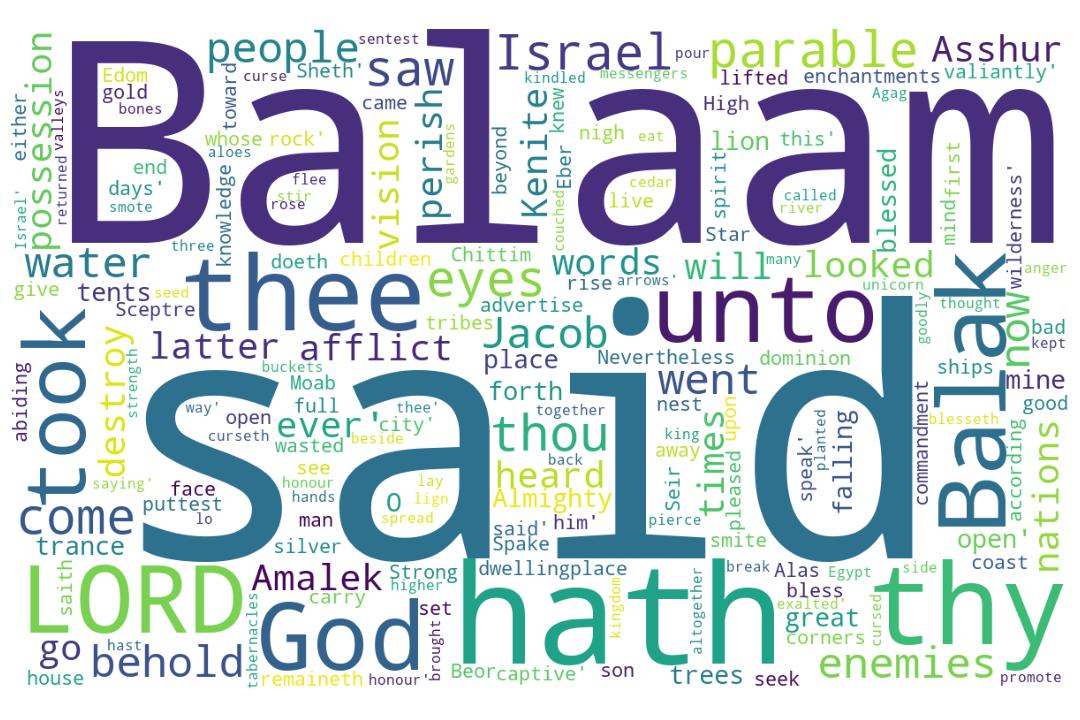
\includegraphics[width=\linewidth]{04OT-Numbers/Numbers24-WordCloud.jpg}
  \caption{Numbers 24 Word Cloud}
  \label{fig:Numbers 24 word Cloud}
\end{figure}

\marginpar{\scriptsize \centering \fcolorbox{bone}{lime}{\textbf{BALAAM'S MINISTRY}}\\ (Numbers 24)
\begin{compactenum}[I.][8]
    \item His \textbf{Compromise} \index[scripture]{Numbers!Num 31:16} (Numbers 31:16) (we find out in Numbers 31 what Balaam's advice was to Balam. The advice is followed in Numbers 25.)
    \item His \textbf{Consideration} \index[scripture]{Numbers!Num 24:01} (Numbers 24:1) 
    \item His \textbf{Coins} \index[scripture]{Jude!Jde 1:11} (Jude 1:11) (his reward)
    \item His \textbf{Corruption} %\index[scripture]{Jude!Jde 1:11} (Jude 1:11) (his reward)
    \item His \textbf{Counsel} \index[scripture]{Numbers!Num 25:03} \index[scripture]{Revelation!Rev 02:14} (Numbers 25:3, Revelation 2:14) (defeat Israel by corrupting them. This happens with the worship of Baal-Peor in Numbers 25. We likely see parallel examples in 21$^{st}$-century Christianity.)
\end{compactenum}}

%%%%%%%%%%%%%%%%%%%%%%%%%%%%%%%%%%
%%%%%%%%%%%%%%%%%%%%%%%%%%%%%%%%%%
\footnote{\textcolor[rgb]{0.00,0.25,0.00}{\hyperlink{NumbersTOC}{Return to end of Table of Contents.}}}\footnote{\href{https://audiobible.com/bible/numbers_24.html}{\textcolor[cmyk]{0.99998,1,0,0}{Numbers 24 Audio}}}\textcolor[cmyk]{0.99998,1,0,0}{\fcolorbox{bone}{bone}{And} when Balaam saw that it pleased the LORD to bless Israel, he went not, as at other times, to seek for enchantments, but he set his face toward the wilderness.}
[2] \textcolor[cmyk]{0.99998,1,0,0}{\fcolorbox{bone}{bone}{And} Balaam lifted up his eyes, and he saw Israel abiding \emph{in} \emph{his} \emph{tents} according to their tribes; and the spirit of God came upon him.}
[3] \textcolor[cmyk]{0.99998,1,0,0}{\fcolorbox{bone}{bone}{And} he took up his parable, and \fcolorbox{bone}{bone}{said}, Balaam the son of Beor hath \fcolorbox{bone}{bone}{said}, and the man whose eyes are open hath \fcolorbox{bone}{bone}{said}:}
[4] \textcolor[cmyk]{0.99998,1,0,0}{He hath \fcolorbox{bone}{bone}{said}, which heard the words of God, which saw the vision of the Almighty, falling \emph{into} \emph{a} \emph{trance}, but having his eyes open:}
[5] \textcolor[cmyk]{0.99998,1,0,0}{How goodly are thy tents, O Jacob, \emph{and} thy tabernacles, O Israel!}
[6] \textcolor[cmyk]{0.99998,1,0,0}{As the valleys are they spread forth, as gardens by the river's side, as the trees of lign aloes which the LORD hath planted, \emph{and} as cedar trees beside the waters.}
[7] \textcolor[cmyk]{0.99998,1,0,0}{He shall pour the water out of his buckets, and his seed \emph{shall} \emph{be} in many waters, and his king shall be higher than Agag, and his kingdom shall be exalted.}
[8] \textcolor[cmyk]{0.99998,1,0,0}{God brought him forth out of Egypt; he hath as it were the strength of an unicorn: he shall eat up the nations his enemies, and shall break their bones, and pierce \emph{them} through with his arrows.}
[9] \textcolor[cmyk]{0.99998,1,0,0}{He couched, he lay down as a lion, and as a great lion: who shall stir him up? Blessed \emph{is} he that blesseth thee, and cursed \emph{is} he that curseth thee.}\\
\\
\P \textcolor[cmyk]{0.99998,1,0,0}{\fcolorbox{bone}{bone}{And} Balak's anger was kindled against Balaam, and he smote his hands together: and Balak \fcolorbox{bone}{bone}{said} unto Balaam, I called thee to curse mine enemies, and, behold, thou hast altogether blessed \emph{them} these three times.}
[11] \textcolor[cmyk]{0.99998,1,0,0}{Therefore now flee thou to thy place: I thought to promote thee unto great honour; but, lo, the LORD hath kept thee back from honour.}
[12] \textcolor[cmyk]{0.99998,1,0,0}{\fcolorbox{bone}{bone}{And} Balaam \fcolorbox{bone}{bone}{said} unto Balak, Spake I not also to thy messengers which thou sentest unto me, saying,}
[13] \textcolor[cmyk]{0.99998,1,0,0}{If Balak would give me his house full of silver and gold, I cannot go beyond the commandment of the LORD, to do \emph{either} good or bad of mine own mind; \emph{but} what the LORD saith, that will I speak?}
[14] \textcolor[cmyk]{0.99998,1,0,0}{\fcolorbox{bone}{bone}{And} now, behold, I go unto my people: come \emph{therefore,} \emph{and} I will advertise thee what this people shall do to thy people in the latter days.}\\
\\
\P \textcolor[cmyk]{0.99998,1,0,0}{\fcolorbox{bone}{bone}{And} he took up his parable, and \fcolorbox{bone}{bone}{said}, Balaam the son of Beor hath \fcolorbox{bone}{bone}{said}, and the man whose eyes are open hath \fcolorbox{bone}{bone}{said}:}
[16] \textcolor[cmyk]{0.99998,1,0,0}{He hath \fcolorbox{bone}{bone}{said}, which heard the words of God, and knew the knowledge of the most High, \emph{which} saw the vision of the Almighty, falling \emph{into} \emph{a} \emph{trance}, but having his eyes open:}
[17] \textcolor[cmyk]{0.99998,1,0,0}{I shall see him, but not now: I shall behold him, but not nigh: there shall come a Star out of Jacob, and a Sceptre shall rise out of Israel, and shall smite the corners of Moab, and destroy all the children of Sheth.}
[18] \textcolor[cmyk]{0.99998,1,0,0}{\fcolorbox{bone}{bone}{And} Edom shall be a possession, Seir also shall be a possession for his enemies; and Israel shall do valiantly.}
[19] \textcolor[cmyk]{0.99998,1,0,0}{Out of Jacob shall come he that shall have dominion, and shall destroy him that remaineth of the city.}\\
\\
\P \textcolor[cmyk]{0.99998,1,0,0}{\fcolorbox{bone}{bone}{And} when he looked on Amalek, he took up his parable, and \fcolorbox{bone}{bone}{said}, Amalek \emph{was} the first of the nations; but his latter end \emph{shall} \emph{be} that he perish for ever.}
[21] \textcolor[cmyk]{0.99998,1,0,0}{\fcolorbox{bone}{bone}{And} he looked on the Kenites, and took up his parable, and \fcolorbox{bone}{bone}{said}, Strong is thy \fcolorbox{bone}{MYGOLD}{dwellingplace}, and thou puttest thy nest in a rock.}
[22] \textcolor[cmyk]{0.99998,1,0,0}{Nevertheless the Kenite shall be wasted, until Asshur shall carry thee away captive.}
[23] \textcolor[cmyk]{0.99998,1,0,0}{\fcolorbox{bone}{bone}{And} he took up his parable, and \fcolorbox{bone}{bone}{said}, Alas, who shall live when God doeth this!}
[24] \textcolor[cmyk]{0.99998,1,0,0}{\fcolorbox{bone}{bone}{And} ships \emph{shall} \emph{come} from the coast of Chittim, and shall afflict Asshur, and shall afflict Eber, and he also shall perish for ever.}
[25] \textcolor[cmyk]{0.99998,1,0,0}{\fcolorbox{bone}{bone}{And} Balaam rose up, and went and returned to his place: and Balak also went his way.}
\index[NWIV]{31!Numbers!Num 24:001}\index[AWIP]{And!Numbers!Num 24:001}\index[AWIP]{when!Numbers!Num 24:001}\index[AWIP]{Balaam!Numbers!Num 24:001}\index[AWIP]{saw!Numbers!Num 24:001}\index[AWIP]{that!Numbers!Num 24:001}\index[AWIP]{it!Numbers!Num 24:001}\index[AWIP]{pleased!Numbers!Num 24:001}\index[AWIP]{the!Numbers!Num 24:001}\index[AWIP]{LORD!Numbers!Num 24:001}\index[AWIP]{to!Numbers!Num 24:001}\index[AWIP]{bless!Numbers!Num 24:001}\index[AWIP]{Israel!Numbers!Num 24:001}\index[AWIP]{he!Numbers!Num 24:001}\index[AWIP]{went!Numbers!Num 24:001}\index[AWIP]{not!Numbers!Num 24:001}\index[AWIP]{as!Numbers!Num 24:001}\index[AWIP]{at!Numbers!Num 24:001}\index[AWIP]{other!Numbers!Num 24:001}\index[AWIP]{times!Numbers!Num 24:001}\index[AWIP]{to!Numbers!Num 24:001 (2)}\index[AWIP]{seek!Numbers!Num 24:001}\index[AWIP]{for!Numbers!Num 24:001}\index[AWIP]{enchantments!Numbers!Num 24:001}\index[AWIP]{but!Numbers!Num 24:001}\index[AWIP]{he!Numbers!Num 24:001 (2)}\index[AWIP]{set!Numbers!Num 24:001}\index[AWIP]{his!Numbers!Num 24:001}\index[AWIP]{face!Numbers!Num 24:001}\index[AWIP]{toward!Numbers!Num 24:001}\index[AWIP]{the!Numbers!Num 24:001 (2)}\index[AWIP]{wilderness!Numbers!Num 24:001}\index[PNIP]{Balaam!Numbers!Num 24:001}\index[PNIP]{LORD!Numbers!Num 24:001}\index[PNIP]{Israel!Numbers!Num 24:001}

\index[NWIV]{26!Numbers!Num 24:002}\index[AWIP]{And!Numbers!Num 24:002}\index[AWIP]{Balaam!Numbers!Num 24:002}\index[AWIP]{lifted!Numbers!Num 24:002}\index[AWIP]{up!Numbers!Num 24:002}\index[AWIP]{his!Numbers!Num 24:002}\index[AWIP]{eyes!Numbers!Num 24:002}\index[AWIP]{and!Numbers!Num 24:002}\index[AWIP]{he!Numbers!Num 24:002}\index[AWIP]{saw!Numbers!Num 24:002}\index[AWIP]{Israel!Numbers!Num 24:002}\index[AWIP]{abiding!Numbers!Num 24:002}\index[AWIP]{\emph{in}!Numbers!Num 24:002}\index[AWIP]{\emph{his}!Numbers!Num 24:002}\index[AWIP]{\emph{tents}!Numbers!Num 24:002}\index[AWIP]{according!Numbers!Num 24:002}\index[AWIP]{to!Numbers!Num 24:002}\index[AWIP]{their!Numbers!Num 24:002}\index[AWIP]{tribes!Numbers!Num 24:002}\index[AWIP]{and!Numbers!Num 24:002 (2)}\index[AWIP]{the!Numbers!Num 24:002}\index[AWIP]{spirit!Numbers!Num 24:002}\index[AWIP]{of!Numbers!Num 24:002}\index[AWIP]{God!Numbers!Num 24:002}\index[AWIP]{came!Numbers!Num 24:002}\index[AWIP]{upon!Numbers!Num 24:002}\index[AWIP]{him!Numbers!Num 24:002}\index[PNIP]{Balaam!Numbers!Num 24:002}\index[PNIP]{Israel!Numbers!Num 24:002}\index[PNIP]{God!Numbers!Num 24:002}

\index[NWIV]{24!Numbers!Num 24:003}\index[AWIP]{And!Numbers!Num 24:003}\index[AWIP]{he!Numbers!Num 24:003}\index[AWIP]{took!Numbers!Num 24:003}\index[AWIP]{up!Numbers!Num 24:003}\index[AWIP]{his!Numbers!Num 24:003}\index[AWIP]{parable!Numbers!Num 24:003}\index[AWIP]{and!Numbers!Num 24:003}\index[AWIP]{said!Numbers!Num 24:003}\index[AWIP]{Balaam!Numbers!Num 24:003}\index[AWIP]{the!Numbers!Num 24:003}\index[AWIP]{son!Numbers!Num 24:003}\index[AWIP]{of!Numbers!Num 24:003}\index[AWIP]{Beor!Numbers!Num 24:003}\index[AWIP]{hath!Numbers!Num 24:003}\index[AWIP]{said!Numbers!Num 24:003 (2)}\index[AWIP]{and!Numbers!Num 24:003 (2)}\index[AWIP]{the!Numbers!Num 24:003 (2)}\index[AWIP]{man!Numbers!Num 24:003}\index[AWIP]{whose!Numbers!Num 24:003}\index[AWIP]{eyes!Numbers!Num 24:003}\index[AWIP]{are!Numbers!Num 24:003}\index[AWIP]{open!Numbers!Num 24:003}\index[AWIP]{hath!Numbers!Num 24:003 (2)}\index[AWIP]{said!Numbers!Num 24:003 (3)}\index[PNIP]{Balaam!Numbers!Num 24:003}\index[PNIP]{Beor!Numbers!Num 24:003}

\index[NWIV]{25!Numbers!Num 24:004}\index[AWIP]{He!Numbers!Num 24:004}\index[AWIP]{hath!Numbers!Num 24:004}\index[AWIP]{said!Numbers!Num 24:004}\index[AWIP]{which!Numbers!Num 24:004}\index[AWIP]{heard!Numbers!Num 24:004}\index[AWIP]{the!Numbers!Num 24:004}\index[AWIP]{words!Numbers!Num 24:004}\index[AWIP]{of!Numbers!Num 24:004}\index[AWIP]{God!Numbers!Num 24:004}\index[AWIP]{which!Numbers!Num 24:004 (2)}\index[AWIP]{saw!Numbers!Num 24:004}\index[AWIP]{the!Numbers!Num 24:004 (2)}\index[AWIP]{vision!Numbers!Num 24:004}\index[AWIP]{of!Numbers!Num 24:004 (2)}\index[AWIP]{the!Numbers!Num 24:004 (3)}\index[AWIP]{Almighty!Numbers!Num 24:004}\index[AWIP]{falling!Numbers!Num 24:004}\index[AWIP]{\emph{into}!Numbers!Num 24:004}\index[AWIP]{\emph{a}!Numbers!Num 24:004}\index[AWIP]{\emph{trance}!Numbers!Num 24:004}\index[AWIP]{but!Numbers!Num 24:004}\index[AWIP]{having!Numbers!Num 24:004}\index[AWIP]{his!Numbers!Num 24:004}\index[AWIP]{eyes!Numbers!Num 24:004}\index[AWIP]{open!Numbers!Num 24:004}\index[PNIP]{God!Numbers!Num 24:004}

\index[NWIV]{12!Numbers!Num 24:005}\index[AWIP]{How!Numbers!Num 24:005}\index[AWIP]{goodly!Numbers!Num 24:005}\index[AWIP]{are!Numbers!Num 24:005}\index[AWIP]{thy!Numbers!Num 24:005}\index[AWIP]{tents!Numbers!Num 24:005}\index[AWIP]{O!Numbers!Num 24:005}\index[AWIP]{Jacob!Numbers!Num 24:005}\index[AWIP]{\emph{and}!Numbers!Num 24:005}\index[AWIP]{thy!Numbers!Num 24:005 (2)}\index[AWIP]{tabernacles!Numbers!Num 24:005}\index[AWIP]{O!Numbers!Num 24:005 (2)}\index[AWIP]{Israel!Numbers!Num 24:005}\index[PNIP]{Jacob!Numbers!Num 24:005}\index[PNIP]{Israel!Numbers!Num 24:005}

\index[NWIV]{31!Numbers!Num 24:006}\index[AWIP]{As!Numbers!Num 24:006}\index[AWIP]{the!Numbers!Num 24:006}\index[AWIP]{valleys!Numbers!Num 24:006}\index[AWIP]{are!Numbers!Num 24:006}\index[AWIP]{they!Numbers!Num 24:006}\index[AWIP]{spread!Numbers!Num 24:006}\index[AWIP]{forth!Numbers!Num 24:006}\index[AWIP]{as!Numbers!Num 24:006}\index[AWIP]{gardens!Numbers!Num 24:006}\index[AWIP]{by!Numbers!Num 24:006}\index[AWIP]{the!Numbers!Num 24:006 (2)}\index[AWIP]{river's!Numbers!Num 24:006}\index[AWIP]{side!Numbers!Num 24:006}\index[AWIP]{as!Numbers!Num 24:006 (2)}\index[AWIP]{the!Numbers!Num 24:006 (3)}\index[AWIP]{trees!Numbers!Num 24:006}\index[AWIP]{of!Numbers!Num 24:006}\index[AWIP]{lign!Numbers!Num 24:006}\index[AWIP]{aloes!Numbers!Num 24:006}\index[AWIP]{which!Numbers!Num 24:006}\index[AWIP]{the!Numbers!Num 24:006 (4)}\index[AWIP]{LORD!Numbers!Num 24:006}\index[AWIP]{hath!Numbers!Num 24:006}\index[AWIP]{planted!Numbers!Num 24:006}\index[AWIP]{\emph{and}!Numbers!Num 24:006}\index[AWIP]{as!Numbers!Num 24:006 (3)}\index[AWIP]{cedar!Numbers!Num 24:006}\index[AWIP]{trees!Numbers!Num 24:006 (2)}\index[AWIP]{beside!Numbers!Num 24:006}\index[AWIP]{the!Numbers!Num 24:006 (5)}\index[AWIP]{waters!Numbers!Num 24:006}\index[PNIP]{LORD!Numbers!Num 24:006}

\index[NWIV]{31!Numbers!Num 24:007}\index[AWIP]{He!Numbers!Num 24:007}\index[AWIP]{shall!Numbers!Num 24:007}\index[AWIP]{pour!Numbers!Num 24:007}\index[AWIP]{the!Numbers!Num 24:007}\index[AWIP]{water!Numbers!Num 24:007}\index[AWIP]{out!Numbers!Num 24:007}\index[AWIP]{of!Numbers!Num 24:007}\index[AWIP]{his!Numbers!Num 24:007}\index[AWIP]{buckets!Numbers!Num 24:007}\index[AWIP]{and!Numbers!Num 24:007}\index[AWIP]{his!Numbers!Num 24:007 (2)}\index[AWIP]{seed!Numbers!Num 24:007}\index[AWIP]{\emph{shall}!Numbers!Num 24:007}\index[AWIP]{\emph{be}!Numbers!Num 24:007}\index[AWIP]{in!Numbers!Num 24:007}\index[AWIP]{many!Numbers!Num 24:007}\index[AWIP]{waters!Numbers!Num 24:007}\index[AWIP]{and!Numbers!Num 24:007 (2)}\index[AWIP]{his!Numbers!Num 24:007 (3)}\index[AWIP]{king!Numbers!Num 24:007}\index[AWIP]{shall!Numbers!Num 24:007 (2)}\index[AWIP]{be!Numbers!Num 24:007}\index[AWIP]{higher!Numbers!Num 24:007}\index[AWIP]{than!Numbers!Num 24:007}\index[AWIP]{Agag!Numbers!Num 24:007}\index[AWIP]{and!Numbers!Num 24:007 (3)}\index[AWIP]{his!Numbers!Num 24:007 (4)}\index[AWIP]{kingdom!Numbers!Num 24:007}\index[AWIP]{shall!Numbers!Num 24:007 (3)}\index[AWIP]{be!Numbers!Num 24:007 (2)}\index[AWIP]{exalted!Numbers!Num 24:007}

\index[NWIV]{37!Numbers!Num 24:008}\index[AWIP]{God!Numbers!Num 24:008}\index[AWIP]{brought!Numbers!Num 24:008}\index[AWIP]{him!Numbers!Num 24:008}\index[AWIP]{forth!Numbers!Num 24:008}\index[AWIP]{out!Numbers!Num 24:008}\index[AWIP]{of!Numbers!Num 24:008}\index[AWIP]{Egypt!Numbers!Num 24:008}\index[AWIP]{he!Numbers!Num 24:008}\index[AWIP]{hath!Numbers!Num 24:008}\index[AWIP]{as!Numbers!Num 24:008}\index[AWIP]{it!Numbers!Num 24:008}\index[AWIP]{were!Numbers!Num 24:008}\index[AWIP]{the!Numbers!Num 24:008}\index[AWIP]{strength!Numbers!Num 24:008}\index[AWIP]{of!Numbers!Num 24:008 (2)}\index[AWIP]{an!Numbers!Num 24:008}\index[AWIP]{unicorn!Numbers!Num 24:008}\index[AWIP]{he!Numbers!Num 24:008 (2)}\index[AWIP]{shall!Numbers!Num 24:008}\index[AWIP]{eat!Numbers!Num 24:008}\index[AWIP]{up!Numbers!Num 24:008}\index[AWIP]{the!Numbers!Num 24:008 (2)}\index[AWIP]{nations!Numbers!Num 24:008}\index[AWIP]{his!Numbers!Num 24:008}\index[AWIP]{enemies!Numbers!Num 24:008}\index[AWIP]{and!Numbers!Num 24:008}\index[AWIP]{shall!Numbers!Num 24:008 (2)}\index[AWIP]{break!Numbers!Num 24:008}\index[AWIP]{their!Numbers!Num 24:008}\index[AWIP]{bones!Numbers!Num 24:008}\index[AWIP]{and!Numbers!Num 24:008 (2)}\index[AWIP]{pierce!Numbers!Num 24:008}\index[AWIP]{\emph{them}!Numbers!Num 24:008}\index[AWIP]{through!Numbers!Num 24:008}\index[AWIP]{with!Numbers!Num 24:008}\index[AWIP]{his!Numbers!Num 24:008 (2)}\index[AWIP]{arrows!Numbers!Num 24:008}\index[PNIP]{God!Numbers!Num 24:008}\index[PNIP]{Egypt!Numbers!Num 24:008}

\index[NWIV]{31!Numbers!Num 24:009}\index[AWIP]{He!Numbers!Num 24:009}\index[AWIP]{couched!Numbers!Num 24:009}\index[AWIP]{he!Numbers!Num 24:009}\index[AWIP]{lay!Numbers!Num 24:009}\index[AWIP]{down!Numbers!Num 24:009}\index[AWIP]{as!Numbers!Num 24:009}\index[AWIP]{a!Numbers!Num 24:009}\index[AWIP]{lion!Numbers!Num 24:009}\index[AWIP]{and!Numbers!Num 24:009}\index[AWIP]{as!Numbers!Num 24:009 (2)}\index[AWIP]{a!Numbers!Num 24:009 (2)}\index[AWIP]{great!Numbers!Num 24:009}\index[AWIP]{lion!Numbers!Num 24:009 (2)}\index[AWIP]{who!Numbers!Num 24:009}\index[AWIP]{shall!Numbers!Num 24:009}\index[AWIP]{stir!Numbers!Num 24:009}\index[AWIP]{him!Numbers!Num 24:009}\index[AWIP]{up!Numbers!Num 24:009}\index[AWIP]{Blessed!Numbers!Num 24:009}\index[AWIP]{\emph{is}!Numbers!Num 24:009}\index[AWIP]{he!Numbers!Num 24:009 (2)}\index[AWIP]{that!Numbers!Num 24:009}\index[AWIP]{blesseth!Numbers!Num 24:009}\index[AWIP]{thee!Numbers!Num 24:009}\index[AWIP]{and!Numbers!Num 24:009 (2)}\index[AWIP]{cursed!Numbers!Num 24:009}\index[AWIP]{\emph{is}!Numbers!Num 24:009 (2)}\index[AWIP]{he!Numbers!Num 24:009 (3)}\index[AWIP]{that!Numbers!Num 24:009 (2)}\index[AWIP]{curseth!Numbers!Num 24:009}\index[AWIP]{thee!Numbers!Num 24:009 (2)}

\index[NWIV]{35!Numbers!Num 24:010}\index[AWIP]{And!Numbers!Num 24:010}\index[AWIP]{Balak's!Numbers!Num 24:010}\index[AWIP]{anger!Numbers!Num 24:010}\index[AWIP]{was!Numbers!Num 24:010}\index[AWIP]{kindled!Numbers!Num 24:010}\index[AWIP]{against!Numbers!Num 24:010}\index[AWIP]{Balaam!Numbers!Num 24:010}\index[AWIP]{and!Numbers!Num 24:010}\index[AWIP]{he!Numbers!Num 24:010}\index[AWIP]{smote!Numbers!Num 24:010}\index[AWIP]{his!Numbers!Num 24:010}\index[AWIP]{hands!Numbers!Num 24:010}\index[AWIP]{together!Numbers!Num 24:010}\index[AWIP]{and!Numbers!Num 24:010 (2)}\index[AWIP]{Balak!Numbers!Num 24:010}\index[AWIP]{said!Numbers!Num 24:010}\index[AWIP]{unto!Numbers!Num 24:010}\index[AWIP]{Balaam!Numbers!Num 24:010 (2)}\index[AWIP]{I!Numbers!Num 24:010}\index[AWIP]{called!Numbers!Num 24:010}\index[AWIP]{thee!Numbers!Num 24:010}\index[AWIP]{to!Numbers!Num 24:010}\index[AWIP]{curse!Numbers!Num 24:010}\index[AWIP]{mine!Numbers!Num 24:010}\index[AWIP]{enemies!Numbers!Num 24:010}\index[AWIP]{and!Numbers!Num 24:010 (3)}\index[AWIP]{behold!Numbers!Num 24:010}\index[AWIP]{thou!Numbers!Num 24:010}\index[AWIP]{hast!Numbers!Num 24:010}\index[AWIP]{altogether!Numbers!Num 24:010}\index[AWIP]{blessed!Numbers!Num 24:010}\index[AWIP]{\emph{them}!Numbers!Num 24:010}\index[AWIP]{these!Numbers!Num 24:010}\index[AWIP]{three!Numbers!Num 24:010}\index[AWIP]{times!Numbers!Num 24:010}\index[PNIP]{Balaam!Numbers!Num 24:010}\index[PNIP]{Balak!Numbers!Num 24:010}\index[PNIP]{I!Numbers!Num 24:010}

\index[NWIV]{25!Numbers!Num 24:011}\index[AWIP]{Therefore!Numbers!Num 24:011}\index[AWIP]{now!Numbers!Num 24:011}\index[AWIP]{flee!Numbers!Num 24:011}\index[AWIP]{thou!Numbers!Num 24:011}\index[AWIP]{to!Numbers!Num 24:011}\index[AWIP]{thy!Numbers!Num 24:011}\index[AWIP]{place!Numbers!Num 24:011}\index[AWIP]{I!Numbers!Num 24:011}\index[AWIP]{thought!Numbers!Num 24:011}\index[AWIP]{to!Numbers!Num 24:011 (2)}\index[AWIP]{promote!Numbers!Num 24:011}\index[AWIP]{thee!Numbers!Num 24:011}\index[AWIP]{unto!Numbers!Num 24:011}\index[AWIP]{great!Numbers!Num 24:011}\index[AWIP]{honour!Numbers!Num 24:011}\index[AWIP]{but!Numbers!Num 24:011}\index[AWIP]{lo!Numbers!Num 24:011}\index[AWIP]{the!Numbers!Num 24:011}\index[AWIP]{LORD!Numbers!Num 24:011}\index[AWIP]{hath!Numbers!Num 24:011}\index[AWIP]{kept!Numbers!Num 24:011}\index[AWIP]{thee!Numbers!Num 24:011 (2)}\index[AWIP]{back!Numbers!Num 24:011}\index[AWIP]{from!Numbers!Num 24:011}\index[AWIP]{honour!Numbers!Num 24:011 (2)}\index[PNIP]{I!Numbers!Num 24:011}\index[PNIP]{LORD!Numbers!Num 24:011}

\index[NWIV]{18!Numbers!Num 24:012}\index[AWIP]{And!Numbers!Num 24:012}\index[AWIP]{Balaam!Numbers!Num 24:012}\index[AWIP]{said!Numbers!Num 24:012}\index[AWIP]{unto!Numbers!Num 24:012}\index[AWIP]{Balak!Numbers!Num 24:012}\index[AWIP]{Spake!Numbers!Num 24:012}\index[AWIP]{I!Numbers!Num 24:012}\index[AWIP]{not!Numbers!Num 24:012}\index[AWIP]{also!Numbers!Num 24:012}\index[AWIP]{to!Numbers!Num 24:012}\index[AWIP]{thy!Numbers!Num 24:012}\index[AWIP]{messengers!Numbers!Num 24:012}\index[AWIP]{which!Numbers!Num 24:012}\index[AWIP]{thou!Numbers!Num 24:012}\index[AWIP]{sentest!Numbers!Num 24:012}\index[AWIP]{unto!Numbers!Num 24:012 (2)}\index[AWIP]{me!Numbers!Num 24:012}\index[AWIP]{saying!Numbers!Num 24:012}\index[PNIP]{Balaam!Numbers!Num 24:012}\index[PNIP]{Balak!Numbers!Num 24:012}\index[PNIP]{I!Numbers!Num 24:012}

\index[NWIV]{40!Numbers!Num 24:013}\index[AWIP]{If!Numbers!Num 24:013}\index[AWIP]{Balak!Numbers!Num 24:013}\index[AWIP]{would!Numbers!Num 24:013}\index[AWIP]{give!Numbers!Num 24:013}\index[AWIP]{me!Numbers!Num 24:013}\index[AWIP]{his!Numbers!Num 24:013}\index[AWIP]{house!Numbers!Num 24:013}\index[AWIP]{full!Numbers!Num 24:013}\index[AWIP]{of!Numbers!Num 24:013}\index[AWIP]{silver!Numbers!Num 24:013}\index[AWIP]{and!Numbers!Num 24:013}\index[AWIP]{gold!Numbers!Num 24:013}\index[AWIP]{I!Numbers!Num 24:013}\index[AWIP]{cannot!Numbers!Num 24:013}\index[AWIP]{go!Numbers!Num 24:013}\index[AWIP]{beyond!Numbers!Num 24:013}\index[AWIP]{the!Numbers!Num 24:013}\index[AWIP]{commandment!Numbers!Num 24:013}\index[AWIP]{of!Numbers!Num 24:013 (2)}\index[AWIP]{the!Numbers!Num 24:013 (2)}\index[AWIP]{LORD!Numbers!Num 24:013}\index[AWIP]{to!Numbers!Num 24:013}\index[AWIP]{do!Numbers!Num 24:013}\index[AWIP]{\emph{either}!Numbers!Num 24:013}\index[AWIP]{good!Numbers!Num 24:013}\index[AWIP]{or!Numbers!Num 24:013}\index[AWIP]{bad!Numbers!Num 24:013}\index[AWIP]{of!Numbers!Num 24:013 (3)}\index[AWIP]{mine!Numbers!Num 24:013}\index[AWIP]{own!Numbers!Num 24:013}\index[AWIP]{mind!Numbers!Num 24:013}\index[AWIP]{\emph{but}!Numbers!Num 24:013}\index[AWIP]{what!Numbers!Num 24:013}\index[AWIP]{the!Numbers!Num 24:013 (3)}\index[AWIP]{LORD!Numbers!Num 24:013 (2)}\index[AWIP]{saith!Numbers!Num 24:013}\index[AWIP]{that!Numbers!Num 24:013}\index[AWIP]{will!Numbers!Num 24:013}\index[AWIP]{I!Numbers!Num 24:013 (2)}\index[AWIP]{speak!Numbers!Num 24:013}\index[PNIP]{Balak!Numbers!Num 24:013}\index[PNIP]{I!Numbers!Num 24:013}\index[PNIP]{LORD!Numbers!Num 24:013}

\index[NWIV]{27!Numbers!Num 24:014}\index[AWIP]{And!Numbers!Num 24:014}\index[AWIP]{now!Numbers!Num 24:014}\index[AWIP]{behold!Numbers!Num 24:014}\index[AWIP]{I!Numbers!Num 24:014}\index[AWIP]{go!Numbers!Num 24:014}\index[AWIP]{unto!Numbers!Num 24:014}\index[AWIP]{my!Numbers!Num 24:014}\index[AWIP]{people!Numbers!Num 24:014}\index[AWIP]{come!Numbers!Num 24:014}\index[AWIP]{\emph{therefore}!Numbers!Num 24:014}\index[AWIP]{\emph{and}!Numbers!Num 24:014}\index[AWIP]{I!Numbers!Num 24:014 (2)}\index[AWIP]{will!Numbers!Num 24:014}\index[AWIP]{advertise!Numbers!Num 24:014}\index[AWIP]{thee!Numbers!Num 24:014}\index[AWIP]{what!Numbers!Num 24:014}\index[AWIP]{this!Numbers!Num 24:014}\index[AWIP]{people!Numbers!Num 24:014 (2)}\index[AWIP]{shall!Numbers!Num 24:014}\index[AWIP]{do!Numbers!Num 24:014}\index[AWIP]{to!Numbers!Num 24:014}\index[AWIP]{thy!Numbers!Num 24:014}\index[AWIP]{people!Numbers!Num 24:014 (3)}\index[AWIP]{in!Numbers!Num 24:014}\index[AWIP]{the!Numbers!Num 24:014}\index[AWIP]{latter!Numbers!Num 24:014}\index[AWIP]{days!Numbers!Num 24:014}\index[PNIP]{I!Numbers!Num 24:014}

\index[NWIV]{24!Numbers!Num 24:015}\index[AWIP]{And!Numbers!Num 24:015}\index[AWIP]{he!Numbers!Num 24:015}\index[AWIP]{took!Numbers!Num 24:015}\index[AWIP]{up!Numbers!Num 24:015}\index[AWIP]{his!Numbers!Num 24:015}\index[AWIP]{parable!Numbers!Num 24:015}\index[AWIP]{and!Numbers!Num 24:015}\index[AWIP]{said!Numbers!Num 24:015}\index[AWIP]{Balaam!Numbers!Num 24:015}\index[AWIP]{the!Numbers!Num 24:015}\index[AWIP]{son!Numbers!Num 24:015}\index[AWIP]{of!Numbers!Num 24:015}\index[AWIP]{Beor!Numbers!Num 24:015}\index[AWIP]{hath!Numbers!Num 24:015}\index[AWIP]{said!Numbers!Num 24:015 (2)}\index[AWIP]{and!Numbers!Num 24:015 (2)}\index[AWIP]{the!Numbers!Num 24:015 (2)}\index[AWIP]{man!Numbers!Num 24:015}\index[AWIP]{whose!Numbers!Num 24:015}\index[AWIP]{eyes!Numbers!Num 24:015}\index[AWIP]{are!Numbers!Num 24:015}\index[AWIP]{open!Numbers!Num 24:015}\index[AWIP]{hath!Numbers!Num 24:015 (2)}\index[AWIP]{said!Numbers!Num 24:015 (3)}\index[PNIP]{Balaam!Numbers!Num 24:015}\index[PNIP]{Beor!Numbers!Num 24:015}

\index[NWIV]{33!Numbers!Num 24:016}\index[AWIP]{He!Numbers!Num 24:016}\index[AWIP]{hath!Numbers!Num 24:016}\index[AWIP]{said!Numbers!Num 24:016}\index[AWIP]{which!Numbers!Num 24:016}\index[AWIP]{heard!Numbers!Num 24:016}\index[AWIP]{the!Numbers!Num 24:016}\index[AWIP]{words!Numbers!Num 24:016}\index[AWIP]{of!Numbers!Num 24:016}\index[AWIP]{God!Numbers!Num 24:016}\index[AWIP]{and!Numbers!Num 24:016}\index[AWIP]{knew!Numbers!Num 24:016}\index[AWIP]{the!Numbers!Num 24:016 (2)}\index[AWIP]{knowledge!Numbers!Num 24:016}\index[AWIP]{of!Numbers!Num 24:016 (2)}\index[AWIP]{the!Numbers!Num 24:016 (3)}\index[AWIP]{most!Numbers!Num 24:016}\index[AWIP]{High!Numbers!Num 24:016}\index[AWIP]{\emph{which}!Numbers!Num 24:016}\index[AWIP]{saw!Numbers!Num 24:016}\index[AWIP]{the!Numbers!Num 24:016 (4)}\index[AWIP]{vision!Numbers!Num 24:016}\index[AWIP]{of!Numbers!Num 24:016 (3)}\index[AWIP]{the!Numbers!Num 24:016 (5)}\index[AWIP]{Almighty!Numbers!Num 24:016}\index[AWIP]{falling!Numbers!Num 24:016}\index[AWIP]{\emph{into}!Numbers!Num 24:016}\index[AWIP]{\emph{a}!Numbers!Num 24:016}\index[AWIP]{\emph{trance}!Numbers!Num 24:016}\index[AWIP]{but!Numbers!Num 24:016}\index[AWIP]{having!Numbers!Num 24:016}\index[AWIP]{his!Numbers!Num 24:016}\index[AWIP]{eyes!Numbers!Num 24:016}\index[AWIP]{open!Numbers!Num 24:016}\index[PNIP]{God!Numbers!Num 24:016}\index[PNIP]{High!Numbers!Num 24:016}

\index[NWIV]{44!Numbers!Num 24:017}\index[AWIP]{I!Numbers!Num 24:017}\index[AWIP]{shall!Numbers!Num 24:017}\index[AWIP]{see!Numbers!Num 24:017}\index[AWIP]{him!Numbers!Num 24:017}\index[AWIP]{but!Numbers!Num 24:017}\index[AWIP]{not!Numbers!Num 24:017}\index[AWIP]{now!Numbers!Num 24:017}\index[AWIP]{I!Numbers!Num 24:017 (2)}\index[AWIP]{shall!Numbers!Num 24:017 (2)}\index[AWIP]{behold!Numbers!Num 24:017}\index[AWIP]{him!Numbers!Num 24:017 (2)}\index[AWIP]{but!Numbers!Num 24:017 (2)}\index[AWIP]{not!Numbers!Num 24:017 (2)}\index[AWIP]{nigh!Numbers!Num 24:017}\index[AWIP]{there!Numbers!Num 24:017}\index[AWIP]{shall!Numbers!Num 24:017 (3)}\index[AWIP]{come!Numbers!Num 24:017}\index[AWIP]{a!Numbers!Num 24:017}\index[AWIP]{Star!Numbers!Num 24:017}\index[AWIP]{out!Numbers!Num 24:017}\index[AWIP]{of!Numbers!Num 24:017}\index[AWIP]{Jacob!Numbers!Num 24:017}\index[AWIP]{and!Numbers!Num 24:017}\index[AWIP]{a!Numbers!Num 24:017 (2)}\index[AWIP]{Sceptre!Numbers!Num 24:017}\index[AWIP]{shall!Numbers!Num 24:017 (4)}\index[AWIP]{rise!Numbers!Num 24:017}\index[AWIP]{out!Numbers!Num 24:017 (2)}\index[AWIP]{of!Numbers!Num 24:017 (2)}\index[AWIP]{Israel!Numbers!Num 24:017}\index[AWIP]{and!Numbers!Num 24:017 (2)}\index[AWIP]{shall!Numbers!Num 24:017 (5)}\index[AWIP]{smite!Numbers!Num 24:017}\index[AWIP]{the!Numbers!Num 24:017}\index[AWIP]{corners!Numbers!Num 24:017}\index[AWIP]{of!Numbers!Num 24:017 (3)}\index[AWIP]{Moab!Numbers!Num 24:017}\index[AWIP]{and!Numbers!Num 24:017 (3)}\index[AWIP]{destroy!Numbers!Num 24:017}\index[AWIP]{all!Numbers!Num 24:017}\index[AWIP]{the!Numbers!Num 24:017 (2)}\index[AWIP]{children!Numbers!Num 24:017}\index[AWIP]{of!Numbers!Num 24:017 (4)}\index[AWIP]{Sheth!Numbers!Num 24:017}\index[PNIP]{I!Numbers!Num 24:017}\index[PNIP]{Jacob!Numbers!Num 24:017}\index[PNIP]{Israel!Numbers!Num 24:017}\index[PNIP]{Moab!Numbers!Num 24:017}

\index[NWIV]{20!Numbers!Num 24:018}\index[AWIP]{And!Numbers!Num 24:018}\index[AWIP]{Edom!Numbers!Num 24:018}\index[AWIP]{shall!Numbers!Num 24:018}\index[AWIP]{be!Numbers!Num 24:018}\index[AWIP]{a!Numbers!Num 24:018}\index[AWIP]{possession!Numbers!Num 24:018}\index[AWIP]{Seir!Numbers!Num 24:018}\index[AWIP]{also!Numbers!Num 24:018}\index[AWIP]{shall!Numbers!Num 24:018 (2)}\index[AWIP]{be!Numbers!Num 24:018 (2)}\index[AWIP]{a!Numbers!Num 24:018 (2)}\index[AWIP]{possession!Numbers!Num 24:018 (2)}\index[AWIP]{for!Numbers!Num 24:018}\index[AWIP]{his!Numbers!Num 24:018}\index[AWIP]{enemies!Numbers!Num 24:018}\index[AWIP]{and!Numbers!Num 24:018}\index[AWIP]{Israel!Numbers!Num 24:018}\index[AWIP]{shall!Numbers!Num 24:018 (3)}\index[AWIP]{do!Numbers!Num 24:018}\index[AWIP]{valiantly!Numbers!Num 24:018}\index[PNIP]{Edom!Numbers!Num 24:018}\index[PNIP]{Israel!Numbers!Num 24:018}

\index[NWIV]{19!Numbers!Num 24:019}\index[AWIP]{Out!Numbers!Num 24:019}\index[AWIP]{of!Numbers!Num 24:019}\index[AWIP]{Jacob!Numbers!Num 24:019}\index[AWIP]{shall!Numbers!Num 24:019}\index[AWIP]{come!Numbers!Num 24:019}\index[AWIP]{he!Numbers!Num 24:019}\index[AWIP]{that!Numbers!Num 24:019}\index[AWIP]{shall!Numbers!Num 24:019 (2)}\index[AWIP]{have!Numbers!Num 24:019}\index[AWIP]{dominion!Numbers!Num 24:019}\index[AWIP]{and!Numbers!Num 24:019}\index[AWIP]{shall!Numbers!Num 24:019 (3)}\index[AWIP]{destroy!Numbers!Num 24:019}\index[AWIP]{him!Numbers!Num 24:019}\index[AWIP]{that!Numbers!Num 24:019 (2)}\index[AWIP]{remaineth!Numbers!Num 24:019}\index[AWIP]{of!Numbers!Num 24:019 (2)}\index[AWIP]{the!Numbers!Num 24:019}\index[AWIP]{city!Numbers!Num 24:019}\index[PNIP]{Jacob!Numbers!Num 24:019}

\index[NWIV]{31!Numbers!Num 24:020}\index[AWIP]{And!Numbers!Num 24:020}\index[AWIP]{when!Numbers!Num 24:020}\index[AWIP]{he!Numbers!Num 24:020}\index[AWIP]{looked!Numbers!Num 24:020}\index[AWIP]{on!Numbers!Num 24:020}\index[AWIP]{Amalek!Numbers!Num 24:020}\index[AWIP]{he!Numbers!Num 24:020 (2)}\index[AWIP]{took!Numbers!Num 24:020}\index[AWIP]{up!Numbers!Num 24:020}\index[AWIP]{his!Numbers!Num 24:020}\index[AWIP]{parable!Numbers!Num 24:020}\index[AWIP]{and!Numbers!Num 24:020}\index[AWIP]{said!Numbers!Num 24:020}\index[AWIP]{Amalek!Numbers!Num 24:020 (2)}\index[AWIP]{\emph{was}!Numbers!Num 24:020}\index[AWIP]{the!Numbers!Num 24:020}\index[AWIP]{first!Numbers!Num 24:020}\index[AWIP]{of!Numbers!Num 24:020}\index[AWIP]{the!Numbers!Num 24:020 (2)}\index[AWIP]{nations!Numbers!Num 24:020}\index[AWIP]{but!Numbers!Num 24:020}\index[AWIP]{his!Numbers!Num 24:020 (2)}\index[AWIP]{latter!Numbers!Num 24:020}\index[AWIP]{end!Numbers!Num 24:020}\index[AWIP]{\emph{shall}!Numbers!Num 24:020}\index[AWIP]{\emph{be}!Numbers!Num 24:020}\index[AWIP]{that!Numbers!Num 24:020}\index[AWIP]{he!Numbers!Num 24:020 (3)}\index[AWIP]{perish!Numbers!Num 24:020}\index[AWIP]{for!Numbers!Num 24:020}\index[AWIP]{ever!Numbers!Num 24:020}\index[PNIP]{Amalek!Numbers!Num 24:020}

\index[NWIV]{25!Numbers!Num 24:021}\index[AWIP]{And!Numbers!Num 24:021}\index[AWIP]{he!Numbers!Num 24:021}\index[AWIP]{looked!Numbers!Num 24:021}\index[AWIP]{on!Numbers!Num 24:021}\index[AWIP]{the!Numbers!Num 24:021}\index[AWIP]{Kenites!Numbers!Num 24:021}\index[AWIP]{and!Numbers!Num 24:021}\index[AWIP]{took!Numbers!Num 24:021}\index[AWIP]{up!Numbers!Num 24:021}\index[AWIP]{his!Numbers!Num 24:021}\index[AWIP]{parable!Numbers!Num 24:021}\index[AWIP]{and!Numbers!Num 24:021 (2)}\index[AWIP]{said!Numbers!Num 24:021}\index[AWIP]{Strong!Numbers!Num 24:021}\index[AWIP]{is!Numbers!Num 24:021}\index[AWIP]{thy!Numbers!Num 24:021}\index[AWIP]{dwellingplace!Numbers!Num 24:021}\index[AWIP]{and!Numbers!Num 24:021 (3)}\index[AWIP]{thou!Numbers!Num 24:021}\index[AWIP]{puttest!Numbers!Num 24:021}\index[AWIP]{thy!Numbers!Num 24:021 (2)}\index[AWIP]{nest!Numbers!Num 24:021}\index[AWIP]{in!Numbers!Num 24:021}\index[AWIP]{a!Numbers!Num 24:021}\index[AWIP]{rock!Numbers!Num 24:021}

\index[NWIV]{13!Numbers!Num 24:022}\index[AWIP]{Nevertheless!Numbers!Num 24:022}\index[AWIP]{the!Numbers!Num 24:022}\index[AWIP]{Kenite!Numbers!Num 24:022}\index[AWIP]{shall!Numbers!Num 24:022}\index[AWIP]{be!Numbers!Num 24:022}\index[AWIP]{wasted!Numbers!Num 24:022}\index[AWIP]{until!Numbers!Num 24:022}\index[AWIP]{Asshur!Numbers!Num 24:022}\index[AWIP]{shall!Numbers!Num 24:022 (2)}\index[AWIP]{carry!Numbers!Num 24:022}\index[AWIP]{thee!Numbers!Num 24:022}\index[AWIP]{away!Numbers!Num 24:022}\index[AWIP]{captive!Numbers!Num 24:022}

\index[NWIV]{16!Numbers!Num 24:023}\index[AWIP]{And!Numbers!Num 24:023}\index[AWIP]{he!Numbers!Num 24:023}\index[AWIP]{took!Numbers!Num 24:023}\index[AWIP]{up!Numbers!Num 24:023}\index[AWIP]{his!Numbers!Num 24:023}\index[AWIP]{parable!Numbers!Num 24:023}\index[AWIP]{and!Numbers!Num 24:023}\index[AWIP]{said!Numbers!Num 24:023}\index[AWIP]{Alas!Numbers!Num 24:023}\index[AWIP]{who!Numbers!Num 24:023}\index[AWIP]{shall!Numbers!Num 24:023}\index[AWIP]{live!Numbers!Num 24:023}\index[AWIP]{when!Numbers!Num 24:023}\index[AWIP]{God!Numbers!Num 24:023}\index[AWIP]{doeth!Numbers!Num 24:023}\index[AWIP]{this!Numbers!Num 24:023}\index[PNIP]{God!Numbers!Num 24:023}

\index[NWIV]{24!Numbers!Num 24:024}\index[AWIP]{And!Numbers!Num 24:024}\index[AWIP]{ships!Numbers!Num 24:024}\index[AWIP]{\emph{shall}!Numbers!Num 24:024}\index[AWIP]{\emph{come}!Numbers!Num 24:024}\index[AWIP]{from!Numbers!Num 24:024}\index[AWIP]{the!Numbers!Num 24:024}\index[AWIP]{coast!Numbers!Num 24:024}\index[AWIP]{of!Numbers!Num 24:024}\index[AWIP]{Chittim!Numbers!Num 24:024}\index[AWIP]{and!Numbers!Num 24:024}\index[AWIP]{shall!Numbers!Num 24:024}\index[AWIP]{afflict!Numbers!Num 24:024}\index[AWIP]{Asshur!Numbers!Num 24:024}\index[AWIP]{and!Numbers!Num 24:024 (2)}\index[AWIP]{shall!Numbers!Num 24:024 (2)}\index[AWIP]{afflict!Numbers!Num 24:024 (2)}\index[AWIP]{Eber!Numbers!Num 24:024}\index[AWIP]{and!Numbers!Num 24:024 (3)}\index[AWIP]{he!Numbers!Num 24:024}\index[AWIP]{also!Numbers!Num 24:024}\index[AWIP]{shall!Numbers!Num 24:024 (3)}\index[AWIP]{perish!Numbers!Num 24:024}\index[AWIP]{for!Numbers!Num 24:024}\index[AWIP]{ever!Numbers!Num 24:024}\index[PNIP]{Chittim!Numbers!Num 24:024}

\index[NWIV]{17!Numbers!Num 24:025}\index[AWIP]{And!Numbers!Num 24:025}\index[AWIP]{Balaam!Numbers!Num 24:025}\index[AWIP]{rose!Numbers!Num 24:025}\index[AWIP]{up!Numbers!Num 24:025}\index[AWIP]{and!Numbers!Num 24:025}\index[AWIP]{went!Numbers!Num 24:025}\index[AWIP]{and!Numbers!Num 24:025 (2)}\index[AWIP]{returned!Numbers!Num 24:025}\index[AWIP]{to!Numbers!Num 24:025}\index[AWIP]{his!Numbers!Num 24:025}\index[AWIP]{place!Numbers!Num 24:025}\index[AWIP]{and!Numbers!Num 24:025 (3)}\index[AWIP]{Balak!Numbers!Num 24:025}\index[AWIP]{also!Numbers!Num 24:025}\index[AWIP]{went!Numbers!Num 24:025 (2)}\index[AWIP]{his!Numbers!Num 24:025 (2)}\index[AWIP]{way!Numbers!Num 24:025}\index[PNIP]{Balaam!Numbers!Num 24:025}\index[PNIP]{Balak!Numbers!Num 24:025}


\section{Numbers 24 Outlines}

\subsection{My Outlines}

\subsubsection{The Ministry of Balaam}
%\textbf{Introduction:} Psalm 48:\footnote{22 July 2016, Keith Anthony.}
\index[speaker]{Keith Anthony!Numbers 24 (The Ministry of Balaam)}
\index[series]{Numbers (Keith Anthony)!Numbers 24 (The Ministry of Balaam)}
\index[date]{2017/02/17!Numbers 24 (The Ministry of Balaam) (Keith Anthony)}
\begin{compactenum}[I.][8]
    \item His \textbf{Compromise} \index[scripture]{Numbers!Num 31:16} (Numbers 31:16) (we find out in Numbers 31 what Balaam's advice was to Balam. The advice is followed in Numbers 25.)
    \item His \textbf{Consideration} \index[scripture]{Numbers!Num 24:01} (Numbers 24:1) 
    \item His \textbf{Coins} \index[scripture]{Jude!Jde 1:11} (Jude 1:11) (his reward)
    \item His \textbf{Corruption} %\index[scripture]{Jude!Jde 1:11} (Jude 1:11) (his reward)
    \item His \textbf{Counsel} \index[scripture]{Numbers!Num 25:03} \index[scripture]{Revelation!Rev 02:14} (Numbers 25:3, Revelation 2:14) (defeat Israel by corrupting them. This happens with the worship of Baal-Peor in Numbers 25. We likely see parallel examples in 21$^{st}$-century Christianity.)
\end{compactenum}


\subsection{Outlines from Others}
\section{Numbers 24 Comments}

\subsection{Numeric Nuggets}
\textbf{13: } Verse 22 has 13 words. Verse 25 has 13 unique words.  The words ``And'' and ``said'' are used 13 times in the chapter. The 13-letter word ``dwellingplace'' is used in the chapter.



\chapter{Psalm 48}

\begin{figure}
  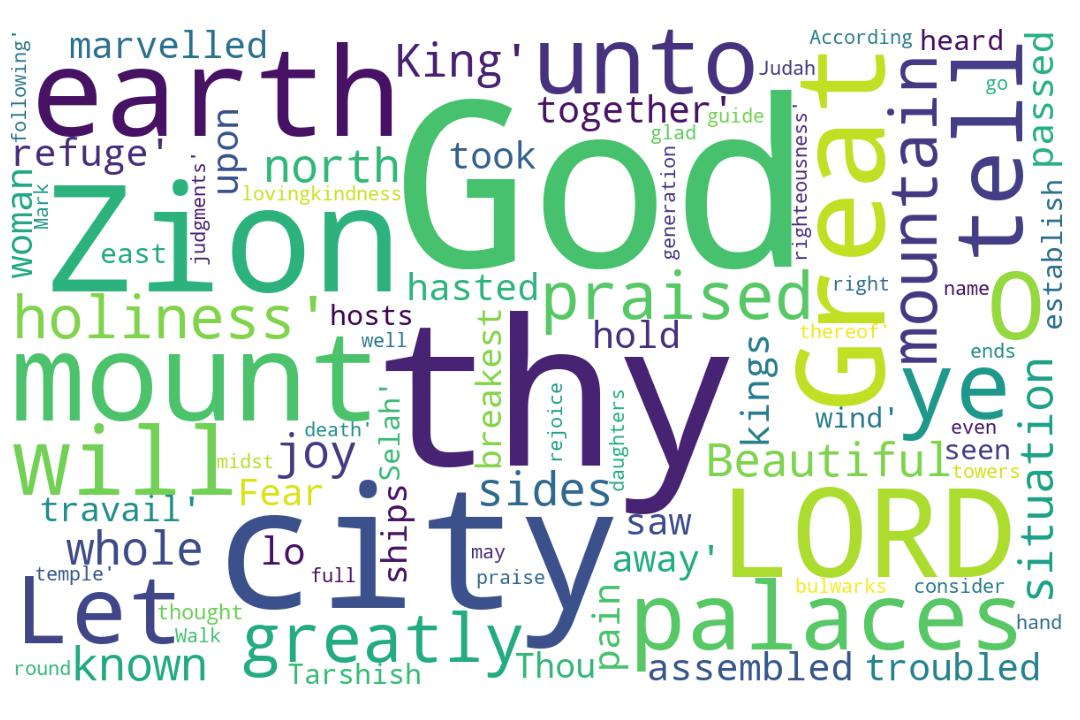
\includegraphics[width=\linewidth]{19OT-Psalms/Psalm48-WordCloud.jpg}
  \caption{Psalm 48 Word Cloud}
  \label{fig:Psalm 48 word Cloud}
\end{figure}



\marginpar{\scriptsize \centering \fcolorbox{bone}{lime}{\textbf{GOD, HIS THRONE, HIS CITY}}\\ (Psalm 48:1-14) \begin{compactenum}[I.][8]
    \item His \textbf{Greatness} \index[scripture]{Psalms!Psa 048:01}(Psa 48:1)
    \item His \textbf{Geography} \index[scripture]{Psalms!Psa 048:02}(Psa 48:2)
    \item Our \textbf{Refuge} \index[scripture]{Psalms!Psa 048:03}(Psa 48:3)
    \item His \textbf{Goodness} \index[scripture]{Psalms!Psa 048:09}(Psa 48:9)
    \item Our \textbf{Gladness} \index[scripture]{Psalms!Psa 048:11}(Psa 48:11)
    \item His \textbf{Glorification} \index[scripture]{Psalms!Psa 048:10}(Psa 48:10)
    \item Our \textbf{Guide} \index[scripture]{Psalms!Psa 048:14}(Psa 48:14)
\end{compactenum}}
    
%%%%%%%%%%%%%%%%%%%%%%%%%%%%%%
%%%%%%%%%%%%%%%%%%%%%%%%%%%%%%
\footnote{\textcolor[cmyk]{0.99998,1,0,0}{\hyperlink{TOC}{Return to end of Table of Contents.}}}\footnote{\href{https://audiobible.com/bible/psalms_48.html}{\textcolor[cmyk]{0.99998,1,0,0}{Psalms Audio}}}\textcolor[cmyk]{0.99998,1,0,0}{A Song \emph{and} Psalm for the sons of Korah.}\\
\\
\textcolor[cmyk]{0.99998,1,0,0}{\fcolorbox{bone}{lime}{Great} \emph{is} the LORD, and greatly to be praised in the city of our God, \emph{in} the mountain of his holiness.}
[2] \textcolor[cmyk]{0.99998,1,0,0}{Beautiful for situation, the joy of the \fcolorbox{bone}{lime}{whole earth}, \emph{is} mount Zion, \emph{on} the sides of the north, the city of the great King.}
[3] \textcolor[cmyk]{0.99998,1,0,0}{God is known in her palaces for a \fcolorbox{bone}{lime}{refuge}.}
[4] \textcolor[cmyk]{0.99998,1,0,0}{For, lo, the kings were assembled, they passed by together.}
[5] \textcolor[cmyk]{0.99998,1,0,0}{They saw \emph{it,} \emph{and} so they marvelled; they were troubled, \emph{and} hasted away.}
[6] \textcolor[cmyk]{0.99998,1,0,0}{Fear took hold upon them there, \emph{and} pain, as of a woman in travail.}
[7] \textcolor[cmyk]{0.99998,1,0,0}{Thou breakest the ships of Tarshish with an east wind.}
[8] \textcolor[cmyk]{0.99998,1,0,0}{As we have heard, so have we seen in the city of the LORD of hosts, in the city of our God: God will establish it for ever. Selah.}
[9] \textcolor[cmyk]{0.99998,1,0,0}{We have thought of thy \fcolorbox{bone}{lime}{lovingkindness}, O God, in the midst of thy temple.}
[10] \textcolor[cmyk]{0.99998,1,0,0}{According to thy name, O God, so \emph{is} thy \fcolorbox{bone}{lime}{praise} unto the ends of the earth: thy right hand is full of \fcolorbox{bone}{MYGOLD}{righteousness}.}
[11] \textcolor[cmyk]{0.99998,1,0,0}{Let mount Zion rejoice, let the daughters of Judah be \fcolorbox{bone}{lime}{glad}, because of thy judgments.}
[12] \textcolor[cmyk]{0.99998,1,0,0}{Walk about Zion, and go round about her: tell the towers thereof.}
[13] \textcolor[cmyk]{0.99998,1,0,0}{Mark ye well her bulwarks, consider her palaces; that ye may tell \emph{it} to the generation following.}
[14] \textcolor[cmyk]{0.99998,1,0,0}{For this God \emph{is} our God for ever and ever: he will be our \fcolorbox{bone}{lime}{guide} \emph{even} unto death.}
\index[NWIV]{21!Psalms!Psa 48:1}\index[AWIP]{Great!Psalms!Psa 48:1}\index[AWIP]{\emph{is}!Psalms!Psa 48:1}\index[AWIP]{the!Psalms!Psa 48:1}\index[AWIP]{the!Psalms!Psa 48:1 (2)}\index[AWIP]{the!Psalms!Psa 48:1 (3)}\index[AWIP]{LORD!Psalms!Psa 48:1}\index[AWIP]{and!Psalms!Psa 48:1}\index[AWIP]{greatly!Psalms!Psa 48:1}\index[AWIP]{to!Psalms!Psa 48:1}\index[AWIP]{be!Psalms!Psa 48:1}\index[AWIP]{praised!Psalms!Psa 48:1}\index[AWIP]{in!Psalms!Psa 48:1}\index[AWIP]{city!Psalms!Psa 48:1}\index[AWIP]{of!Psalms!Psa 48:1}\index[AWIP]{of!Psalms!Psa 48:1 (2)}\index[AWIP]{our!Psalms!Psa 48:1}\index[AWIP]{God!Psalms!Psa 48:1}\index[AWIP]{\emph{in}!Psalms!Psa 48:1}\index[AWIP]{mountain!Psalms!Psa 48:1}\index[AWIP]{his!Psalms!Psa 48:1}\index[AWIP]{holiness!Psalms!Psa 48:1}\index[AWIP]{\emph{is}!Psalms!Psa 48:1}\index[AWIP]{\emph{in}!Psalms!Psa 48:1}

\index[NWIV]{24!Psalms!Psa 48:2}\index[AWIP]{Beautiful!Psalms!Psa 48:2}\index[AWIP]{for!Psalms!Psa 48:2}\index[AWIP]{situation!Psalms!Psa 48:2}\index[AWIP]{the!Psalms!Psa 48:2}\index[AWIP]{the!Psalms!Psa 48:2 (2)}\index[AWIP]{the!Psalms!Psa 48:2 (3)}\index[AWIP]{the!Psalms!Psa 48:2 (4)}\index[AWIP]{the!Psalms!Psa 48:2 (5)}\index[AWIP]{the!Psalms!Psa 48:2 (6)}\index[AWIP]{joy!Psalms!Psa 48:2}\index[AWIP]{of!Psalms!Psa 48:2}\index[AWIP]{of!Psalms!Psa 48:2 (2)}\index[AWIP]{of!Psalms!Psa 48:2 (3)}\index[AWIP]{whole!Psalms!Psa 48:2}\index[AWIP]{earth!Psalms!Psa 48:2}\index[AWIP]{\emph{is}!Psalms!Psa 48:2}\index[AWIP]{mount!Psalms!Psa 48:2}\index[AWIP]{Zion!Psalms!Psa 48:2}\index[AWIP]{\emph{on}!Psalms!Psa 48:2}\index[AWIP]{sides!Psalms!Psa 48:2}\index[AWIP]{north!Psalms!Psa 48:2}\index[AWIP]{city!Psalms!Psa 48:2}\index[AWIP]{great!Psalms!Psa 48:2}\index[AWIP]{King!Psalms!Psa 48:2}\index[AWIP]{\emph{is}!Psalms!Psa 48:2}\index[AWIP]{\emph{on}!Psalms!Psa 48:2}

\index[NWIV]{9!Psalms!Psa 48:3}\index[AWIP]{God!Psalms!Psa 48:3}\index[AWIP]{is!Psalms!Psa 48:3}\index[AWIP]{known!Psalms!Psa 48:3}\index[AWIP]{in!Psalms!Psa 48:3}\index[AWIP]{her!Psalms!Psa 48:3}\index[AWIP]{palaces!Psalms!Psa 48:3}\index[AWIP]{for!Psalms!Psa 48:3}\index[AWIP]{a!Psalms!Psa 48:3}\index[AWIP]{refuge!Psalms!Psa 48:3}

\index[NWIV]{10!Psalms!Psa 48:4}\index[AWIP]{For!Psalms!Psa 48:4}\index[AWIP]{lo!Psalms!Psa 48:4}\index[AWIP]{the!Psalms!Psa 48:4}\index[AWIP]{kings!Psalms!Psa 48:4}\index[AWIP]{were!Psalms!Psa 48:4}\index[AWIP]{assembled!Psalms!Psa 48:4}\index[AWIP]{they!Psalms!Psa 48:4}\index[AWIP]{passed!Psalms!Psa 48:4}\index[AWIP]{by!Psalms!Psa 48:4}\index[AWIP]{together!Psalms!Psa 48:4}

\index[NWIV]{13!Psalms!Psa 48:5}\index[AWIP]{They!Psalms!Psa 48:5}\index[AWIP]{saw!Psalms!Psa 48:5}\index[AWIP]{\emph{it}!Psalms!Psa 48:5}\index[AWIP]{\emph{and}!Psalms!Psa 48:5}\index[AWIP]{\emph{and}!Psalms!Psa 48:5 (2)}\index[AWIP]{so!Psalms!Psa 48:5}\index[AWIP]{they!Psalms!Psa 48:5}\index[AWIP]{they!Psalms!Psa 48:5 (2)}\index[AWIP]{marvelled!Psalms!Psa 48:5}\index[AWIP]{were!Psalms!Psa 48:5}\index[AWIP]{troubled!Psalms!Psa 48:5}\index[AWIP]{hasted!Psalms!Psa 48:5}\index[AWIP]{away!Psalms!Psa 48:5}\index[AWIP]{\emph{it}!Psalms!Psa 48:5}\index[AWIP]{\emph{and}!Psalms!Psa 48:5}\index[AWIP]{\emph{and}!Psalms!Psa 48:5 (2)}

\index[NWIV]{14!Psalms!Psa 48:6}\index[AWIP]{Fear!Psalms!Psa 48:6}\index[AWIP]{took!Psalms!Psa 48:6}\index[AWIP]{hold!Psalms!Psa 48:6}\index[AWIP]{upon!Psalms!Psa 48:6}\index[AWIP]{them!Psalms!Psa 48:6}\index[AWIP]{there!Psalms!Psa 48:6}\index[AWIP]{\emph{and}!Psalms!Psa 48:6}\index[AWIP]{pain!Psalms!Psa 48:6}\index[AWIP]{as!Psalms!Psa 48:6}\index[AWIP]{of!Psalms!Psa 48:6}\index[AWIP]{a!Psalms!Psa 48:6}\index[AWIP]{woman!Psalms!Psa 48:6}\index[AWIP]{in!Psalms!Psa 48:6}\index[AWIP]{travail!Psalms!Psa 48:6}\index[AWIP]{\emph{and}!Psalms!Psa 48:6}

\index[NWIV]{10!Psalms!Psa 48:7}\index[AWIP]{Thou!Psalms!Psa 48:7}\index[AWIP]{breakest!Psalms!Psa 48:7}\index[AWIP]{the!Psalms!Psa 48:7}\index[AWIP]{ships!Psalms!Psa 48:7}\index[AWIP]{of!Psalms!Psa 48:7}\index[AWIP]{Tarshish!Psalms!Psa 48:7}\index[AWIP]{with!Psalms!Psa 48:7}\index[AWIP]{an!Psalms!Psa 48:7}\index[AWIP]{east!Psalms!Psa 48:7}\index[AWIP]{wind!Psalms!Psa 48:7}

\index[NWIV]{29!Psalms!Psa 48:8}\index[AWIP]{As!Psalms!Psa 48:8}\index[AWIP]{we!Psalms!Psa 48:8}\index[AWIP]{we!Psalms!Psa 48:8 (2)}\index[AWIP]{have!Psalms!Psa 48:8}\index[AWIP]{have!Psalms!Psa 48:8 (2)}\index[AWIP]{heard!Psalms!Psa 48:8}\index[AWIP]{so!Psalms!Psa 48:8}\index[AWIP]{seen!Psalms!Psa 48:8}\index[AWIP]{in!Psalms!Psa 48:8}\index[AWIP]{in!Psalms!Psa 48:8 (2)}\index[AWIP]{the!Psalms!Psa 48:8}\index[AWIP]{the!Psalms!Psa 48:8 (2)}\index[AWIP]{the!Psalms!Psa 48:8 (3)}\index[AWIP]{city!Psalms!Psa 48:8}\index[AWIP]{city!Psalms!Psa 48:8 (2)}\index[AWIP]{of!Psalms!Psa 48:8}\index[AWIP]{of!Psalms!Psa 48:8 (2)}\index[AWIP]{of!Psalms!Psa 48:8 (3)}\index[AWIP]{LORD!Psalms!Psa 48:8}\index[AWIP]{hosts!Psalms!Psa 48:8}\index[AWIP]{our!Psalms!Psa 48:8}\index[AWIP]{God!Psalms!Psa 48:8}\index[AWIP]{God!Psalms!Psa 48:8 (2)}\index[AWIP]{will!Psalms!Psa 48:8}\index[AWIP]{establish!Psalms!Psa 48:8}\index[AWIP]{it!Psalms!Psa 48:8}\index[AWIP]{for!Psalms!Psa 48:8}\index[AWIP]{ever!Psalms!Psa 48:8}\index[AWIP]{Selah!Psalms!Psa 48:8}

\index[NWIV]{14!Psalms!Psa 48:9}\index[AWIP]{We!Psalms!Psa 48:9}\index[AWIP]{have!Psalms!Psa 48:9}\index[AWIP]{thought!Psalms!Psa 48:9}\index[AWIP]{of!Psalms!Psa 48:9}\index[AWIP]{of!Psalms!Psa 48:9 (2)}\index[AWIP]{thy!Psalms!Psa 48:9}\index[AWIP]{thy!Psalms!Psa 48:9 (2)}\index[AWIP]{lovingkindness!Psalms!Psa 48:9}\index[AWIP]{O!Psalms!Psa 48:9}\index[AWIP]{God!Psalms!Psa 48:9}\index[AWIP]{in!Psalms!Psa 48:9}\index[AWIP]{the!Psalms!Psa 48:9}\index[AWIP]{midst!Psalms!Psa 48:9}\index[AWIP]{temple!Psalms!Psa 48:9}

\index[NWIV]{23!Psalms!Psa 48:10}\index[AWIP]{According!Psalms!Psa 48:10}\index[AWIP]{to!Psalms!Psa 48:10}\index[AWIP]{thy!Psalms!Psa 48:10}\index[AWIP]{thy!Psalms!Psa 48:10 (2)}\index[AWIP]{thy!Psalms!Psa 48:10 (3)}\index[AWIP]{name!Psalms!Psa 48:10}\index[AWIP]{O!Psalms!Psa 48:10}\index[AWIP]{God!Psalms!Psa 48:10}\index[AWIP]{so!Psalms!Psa 48:10}\index[AWIP]{\emph{is}!Psalms!Psa 48:10}\index[AWIP]{praise!Psalms!Psa 48:10}\index[AWIP]{unto!Psalms!Psa 48:10}\index[AWIP]{the!Psalms!Psa 48:10}\index[AWIP]{the!Psalms!Psa 48:10 (2)}\index[AWIP]{ends!Psalms!Psa 48:10}\index[AWIP]{of!Psalms!Psa 48:10}\index[AWIP]{of!Psalms!Psa 48:10 (2)}\index[AWIP]{earth!Psalms!Psa 48:10}\index[AWIP]{right!Psalms!Psa 48:10}\index[AWIP]{hand!Psalms!Psa 48:10}\index[AWIP]{is!Psalms!Psa 48:10}\index[AWIP]{full!Psalms!Psa 48:10}\index[AWIP]{righteousness!Psalms!Psa 48:10}\index[AWIP]{\emph{is}!Psalms!Psa 48:10}

\index[NWIV]{15!Psalms!Psa 48:11}\index[AWIP]{Let!Psalms!Psa 48:11}\index[AWIP]{mount!Psalms!Psa 48:11}\index[AWIP]{Zion!Psalms!Psa 48:11}\index[AWIP]{rejoice!Psalms!Psa 48:11}\index[AWIP]{let!Psalms!Psa 48:11}\index[AWIP]{the!Psalms!Psa 48:11}\index[AWIP]{daughters!Psalms!Psa 48:11}\index[AWIP]{of!Psalms!Psa 48:11}\index[AWIP]{of!Psalms!Psa 48:11 (2)}\index[AWIP]{Judah!Psalms!Psa 48:11}\index[AWIP]{be!Psalms!Psa 48:11}\index[AWIP]{glad!Psalms!Psa 48:11}\index[AWIP]{because!Psalms!Psa 48:11}\index[AWIP]{thy!Psalms!Psa 48:11}\index[AWIP]{judgments!Psalms!Psa 48:11}

\index[NWIV]{12!Psalms!Psa 48:12}\index[AWIP]{Walk!Psalms!Psa 48:12}\index[AWIP]{about!Psalms!Psa 48:12}\index[AWIP]{about!Psalms!Psa 48:12 (2)}\index[AWIP]{Zion!Psalms!Psa 48:12}\index[AWIP]{and!Psalms!Psa 48:12}\index[AWIP]{go!Psalms!Psa 48:12}\index[AWIP]{round!Psalms!Psa 48:12}\index[AWIP]{her!Psalms!Psa 48:12}\index[AWIP]{tell!Psalms!Psa 48:12}\index[AWIP]{the!Psalms!Psa 48:12}\index[AWIP]{towers!Psalms!Psa 48:12}\index[AWIP]{thereof!Psalms!Psa 48:12}

\index[NWIV]{17!Psalms!Psa 48:13}\index[AWIP]{Mark!Psalms!Psa 48:13}\index[AWIP]{ye!Psalms!Psa 48:13}\index[AWIP]{ye!Psalms!Psa 48:13 (2)}\index[AWIP]{well!Psalms!Psa 48:13}\index[AWIP]{her!Psalms!Psa 48:13}\index[AWIP]{her!Psalms!Psa 48:13 (2)}\index[AWIP]{bulwarks!Psalms!Psa 48:13}\index[AWIP]{consider!Psalms!Psa 48:13}\index[AWIP]{palaces!Psalms!Psa 48:13}\index[AWIP]{that!Psalms!Psa 48:13}\index[AWIP]{may!Psalms!Psa 48:13}\index[AWIP]{tell!Psalms!Psa 48:13}\index[AWIP]{\emph{it}!Psalms!Psa 48:13}\index[AWIP]{to!Psalms!Psa 48:13}\index[AWIP]{the!Psalms!Psa 48:13}\index[AWIP]{generation!Psalms!Psa 48:13}\index[AWIP]{following!Psalms!Psa 48:13}\index[AWIP]{\emph{it}!Psalms!Psa 48:13}

\index[NWIV]{18!Psalms!Psa 48:14}\index[AWIP]{For!Psalms!Psa 48:14}\index[AWIP]{this!Psalms!Psa 48:14}\index[AWIP]{God!Psalms!Psa 48:14}\index[AWIP]{God!Psalms!Psa 48:14 (2)}\index[AWIP]{\emph{is}!Psalms!Psa 48:14}\index[AWIP]{our!Psalms!Psa 48:14}\index[AWIP]{our!Psalms!Psa 48:14 (2)}\index[AWIP]{for!Psalms!Psa 48:14}\index[AWIP]{ever!Psalms!Psa 48:14}\index[AWIP]{ever!Psalms!Psa 48:14 (2)}\index[AWIP]{and!Psalms!Psa 48:14}\index[AWIP]{he!Psalms!Psa 48:14}\index[AWIP]{will!Psalms!Psa 48:14}\index[AWIP]{be!Psalms!Psa 48:14}\index[AWIP]{guide!Psalms!Psa 48:14}\index[AWIP]{\emph{even}!Psalms!Psa 48:14}\index[AWIP]{unto!Psalms!Psa 48:14}\index[AWIP]{death!Psalms!Psa 48:14}\index[AWIP]{\emph{is}!Psalms!Psa 48:14}\index[AWIP]{\emph{even}!Psalms!Psa 48:14}


\section{Psalm 48 Outlines}

\subsection{My Outlines}

\subsubsection{God, His Throne, His City}
%\textbf{Introduction:} Psalm 48:\footnote{22 July 2016, Keith Anthony.}
\index[speaker]{Keith Anthony!Psalm 048 (God on His Throne in His City)}
\index[series]{Psalms (Keith Anthony)!Psalm 048 (God on His Throne in His City)}
\index[date]{2017/02/17!Psalm 048 (God on His Throne in His City) (Keith Anthony)}
\begin{compactenum}[I.][8]
    \item His \textbf{Greatness} \index[scripture]{Psalms!Psa 048:01}(Psa 48:1)
    \item His \textbf{Geography} \index[scripture]{Psalms!Psa 048:02}(Psa 48:2)
    \item Our \textbf{Refuge} \index[scripture]{Psalms!Psa 048:03}(Psa 48:3)
    \item His \textbf{Goodness} \index[scripture]{Psalms!Psa 048:09}(Psa 48:9)
    \item Our \textbf{Gladness} \index[scripture]{Psalms!Psa 048:11}(Psa 48:11)
    \item His \textbf{Glorification} \index[scripture]{Psalms!Psa 048:10}(Psa 48:10)
    \item Our \textbf{Guide} \index[scripture]{Psalms!Psa 048:14}(Psa 48:14)
\end{compactenum}

\subsection{Outlines from Others}



\section{Psalm 48 Comments}

\subsection{Numeric Nuggets}
\textbf{13:} Verse 5 has 13 words. The thirteen-letter word ``righteousness''  is used in the psalm.

\chapter{Proverb 17}
\begin{figure}
  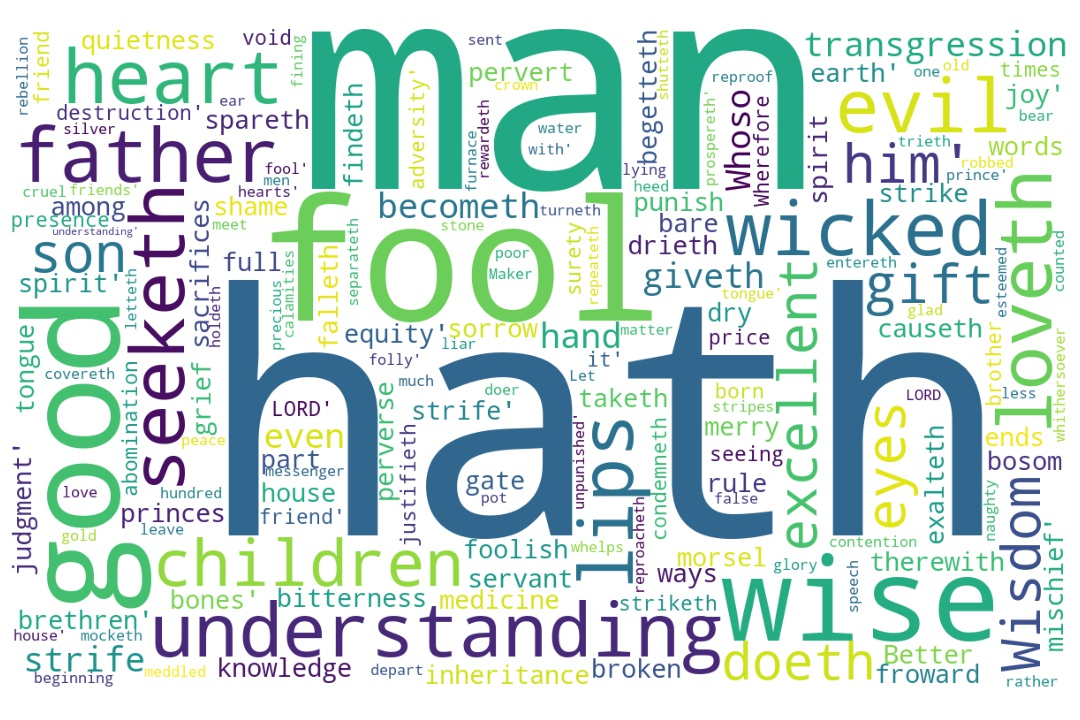
\includegraphics[width=\linewidth]{20OT-Proverbs/Proverb17-WordCloud.jpg}
  \caption{Proverb 17 Word Cloud}
  \label{fig:Proverb 17 word Cloud}
\end{figure}

\marginpar{\scriptsize \centering \fcolorbox{bone}{lime}{\textbf{CONTRASTS}}\\ (Proverbs 17:1-28) \begin{compactenum}[I.][8]
    \item \textbf{A Dry Morsel} \index[scripture]{Proverbs!Pro 17:01}(Pro 17:1) 
    \item \textbf{A Dim-Witted Mocker} \index[scripture]{Proverbs!Pro 17:05}(Pro 17:5) 
    \item \textbf{A Divisive Matter} \index[scripture]{Proverbs!Pro 17:09}(Pro 17:9) 
    \item \textbf{A Disruptive Messenger} \index[scripture]{Proverbs!Pro 17:11}(Pro 17:11) 
    \item \textbf{Destructive Meddling} \index[scripture]{Proverbs!Pro 17:14}(Pro 17:14) 
    \item \textbf{Dangerous Mischief} \index[scripture]{Proverbs!Pro 17:20}(Pro 17:20) 
    \item \textbf{A Discerning Man} \index[scripture]{Proverbs!Pro 17:28} (Pro 17:28) 
\end{compactenum} }

\marginpar{\scriptsize \centering \fcolorbox{bone}{yellow}{\textbf{THE FRUIT OF FOOLS}}\\ (Proverbs 17:1-28) \begin{compactenum}[I.][8]
    \item \textbf{Unwanted Family} \index[scripture]{Proverbs!Pro 17:01}(Pro 17:1) 
    \item \textbf{Unteachable Fool} \index[scripture]{Proverbs!Pro 17:10}(Pro 17:10) 
    \item \textbf{Unstoppable Fool} \index[scripture]{Proverbs!Pro 17:11}(Pro 17:11)  
    \item \textbf{Unrestrained Fanatic} \index[scripture]{Proverbs!Pro 17:11}(Pro 17:11)
    \item \textbf{Uncontrollable Flood} \index[scripture]{Proverbs!Pro 17:14}(Pro 17:14)  
    \item \textbf{Unshakeable Fealty} \index[scripture]{Proverbs!Pro 17:17}(Pro 17:17)  
    \item \textbf{Unfulfilled Father} \index[scripture]{Proverbs!Pro 17:21}(Pro 17:21) 
    \item \textbf{Unobtainable Focus} \index[scripture]{Proverbs!Pro 17:24}(Pro 17:24)  
\end{compactenum} }

\footnote{\textcolor[cmyk]{0.99998,1,0,0}{\hyperlink{TOC}{Return to end of Table of Contents.}}}\footnote{\href{https://audiobible.com/bible/proverbs_17.html}{\textcolor[cmyk]{0.99998,1,0,0}{Proverbs Audio}}}\textcolor[cmyk]{0.99998,1,0,0}{Better \emph{is} a \fcolorbox{bone}{lime}{dry morsel}, and quietness therewith, than an house full of sacrifices \emph{with} strife.}
[2] \textcolor[cmyk]{0.99998,1,0,0}{A wise servant shall have rule over a son that causeth shame, and shall have part of the inheritance among the brethren.}
[3] \textcolor[cmyk]{0.99998,1,0,0}{The fining pot \emph{is} for silver, and the furnace for gold: but the LORD trieth the hearts.}
[4] \textcolor[cmyk]{0.99998,1,0,0}{A wicked doer giveth heed to false lips; \emph{and} a liar giveth ear to a naughty tongue.}
[5] \textcolor[cmyk]{0.99998,1,0,0}{Whoso \fcolorbox{bone}{lime}{mocketh} the poor reproacheth his Maker: \emph{and} he that is glad at calamities shall not be unpunished.}
[6] \textcolor[cmyk]{0.99998,1,0,0}{Children's children \emph{are} the crown of old men; and the glory of children \emph{are} their fathers.}
[7] \textcolor[cmyk]{0.99998,1,0,0}{Excellent speech becometh not a fool: much less do lying lips a prince.}
[8] \textcolor[cmyk]{0.99998,1,0,0}{A gift \emph{is} \emph{as} a precious stone in the eyes of him that hath it: \fcolorbox{bone}{MYGOLD}{whithersoever} it turneth, it prospereth.}
[9] \textcolor[cmyk]{0.99998,1,0,0}{He that covereth a \fcolorbox{bone}{MYGOLD}{transgression} seeketh love; but he that repeateth a matter \fcolorbox{bone}{lime}{separateth} \emph{very} friends.}
[10] \textcolor[cmyk]{0.99998,1,0,0}{A reproof entereth more into a wise man than an hundred stripes into a fool.}
[11] \textcolor[cmyk]{0.99998,1,0,0}{An evil \emph{man} seeketh only rebellion: therefore a \fcolorbox{bone}{lime}{cruel messenger} shall be sent against him.}
[12] \textcolor[cmyk]{0.99998,1,0,0}{Let a bear robbed of her whelps meet a man, rather than a fool in his folly.}
[13] \textcolor[cmyk]{0.99998,1,0,0}{Whoso rewardeth evil for good, evil shall not depart from his house.}
[14] \textcolor[cmyk]{0.99998,1,0,0}{The beginning of strife \emph{is} \emph{as} when one letteth out water: therefore leave off contention, before it be \fcolorbox{bone}{lime}{meddled} with.}
[15] \textcolor[cmyk]{0.99998,1,0,0}{He that justifieth the wicked, and he that condemneth the just, even they both \emph{are} abomination to the LORD.}
[16] \textcolor[cmyk]{0.99998,1,0,0}{Wherefore \emph{is} \emph{there} a price in the hand of a fool to get wisdom, seeing \emph{he} \emph{hath} no heart \emph{to} \emph{it}?}
[17] \textcolor[cmyk]{0.99998,1,0,0}{A friend loveth at all times, and a brother is born for adversity.}
[18] \textcolor[cmyk]{0.99998,1,0,0}{A man void of \fcolorbox{bone}{MYGOLD}{understanding} striketh hands, \emph{and} becometh surety in the presence of his friend.}
[19] \textcolor[cmyk]{0.99998,1,0,0}{He loveth \fcolorbox{bone}{MYGOLD}{transgression} that loveth strife: \emph{and} he that exalteth his gate seeketh destruction.}
[20] \textcolor[cmyk]{0.99998,1,0,0}{He that hath a froward heart findeth no good: and he that hath a perverse tongue falleth into \fcolorbox{bone}{lime}{mischief}.}
[21] \textcolor[cmyk]{0.99998,1,0,0}{He that begetteth a fool \emph{doeth} \emph{it} to his sorrow: and the father of a fool hath no joy.}
[22] \textcolor[cmyk]{0.99998,1,0,0}{A merry heart doeth good \emph{like} a medicine: but a broken spirit drieth the bones.}
[23] \textcolor[cmyk]{0.99998,1,0,0}{A wicked \emph{man} taketh a gift out of the bosom to pervert the ways of judgment.}
[24] \textcolor[cmyk]{0.99998,1,0,0}{Wisdom \emph{is} before him that hath \fcolorbox{bone}{MYGOLD}{understanding}; but the eyes of a fool \emph{are} in the ends of the earth.}
[25] \textcolor[cmyk]{0.99998,1,0,0}{A foolish son \emph{is} a grief to his father, and bitterness to her that bare him.}
[26] \textcolor[cmyk]{0.99998,1,0,0}{Also to punish the just \emph{is} not good, \emph{nor} to strike princes for equity.}
[27] \textcolor[cmyk]{0.99998,1,0,0}{He that hath knowledge spareth his words: \emph{and} a man of \fcolorbox{bone}{MYGOLD}{understanding} is of an excellent spirit.}
[28] \textcolor[cmyk]{0.99998,1,0,0}{Even a fool, when he holdeth his peace, is counted wise: \emph{and} he that shutteth his lips \emph{is} \emph{esteemed} \fcolorbox{bone}{lime}{a man of \fcolorbox{bone}{MYGOLD}{understanding}}.}



\subsection{Proverb 17 Repeated Phrases}


%%%%%%%%%%
%%%%%%%%%%
\normalsize
 
\begin{center}
\begin{longtable}{|c|c|}
\caption[Proverb 17 Repeated Phrases]{Proverb 17 Repeated Phrases}\label{table:Repeated Phrases Proverb 17} \\
\hline \multicolumn{1}{|c|}{\textbf{Phrase}} & \multicolumn{1}{c|}{\textbf{Frequency}} \\ \hline 
\endfirsthead
 
\multicolumn{2}{c}
{{\bfseries \tablename\ \thetable{} -- continued from previous page}} \\  
\hline \multicolumn{1}{|c|}{\textbf{Phrase}} & \multicolumn{1}{c|}{\textbf{Frequency}} \\ \hline 
\endhead
 
\hline \multicolumn{2}{c}{{ }} \\ \hline
\endfoot 
a fool & 8\\ \hline 
he that & 6\\ \hline 
that hath & 5\\ \hline 
He that & 5\\ \hline 
in the & 4\\ \hline 
of the & 3\\ \hline 
and the & 3\\ \hline 
\emph{and} he & 3\\ \hline 
\emph{and} he that & 3\\ \hline 
a man & 3\\ \hline 
of a & 3\\ \hline 
of a fool & 3\\ \hline 
of understanding & 3\\ \hline 
\end{longtable}
\end{center}



%%%%%%%%%%
%%%%%%%%%%



\section{Proverb 17 Outlines}

\subsection{My Outlines}



\subsubsection{Contrasts}
%Proverbs 17:\footnote{18 August 2015, Keith Anthony} 
\index[speaker]{Keith Anthony!Proverb 17 (Contrasts)}
\index[series]{Proverbs (Keith Anthony)!Pro 17 (Contrasts)}
\index[date]{2015/09/17!Proverb 17 (Contrasts) (Keith Anthony)}
\begin{compactenum}[I.]
    \item \textbf{A Dry Morsel} \index[scripture]{Proverbs!Pro 17:01}(Pro 17:1) 
    \item \textbf{A Dim-Witted Mocker} \index[scripture]{Proverbs!Pro 17:05}(Pro 17:5) 
    \item \textbf{A Divisive Matter} \index[scripture]{Proverbs!Pro 17:09}(Pro 17:9) 
    \item \textbf{A Disruptive Messenger} \index[scripture]{Proverbs!Pro 17:11}(Pro 17:11) 
    \item \textbf{Destructive Meddling} \index[scripture]{Proverbs!Pro 17:14}(Pro 17:14) 
    \item \textbf{Dangerous Mischief} \index[scripture]{Proverbs!Pro 17:20}(Pro 17:20) 
    \item \textbf{A Discerning Man} \index[scripture]{Proverbs!Pro 17:28} (Pro 17:28) 
\end{compactenum}

\subsubsection{The Fruit of Fools}
We all have exhibited foolishness in our lives, but hopefully we are not living Lives of Foolishness. There is much in Proverbs 17, but focusing on fools and folly, for now, we see:%\footnote{17 October 20144, Keith Anthony}
\index[speaker]{Keith Anthony!Proverb 17 (The Fruit of Fools)}
\index[series]{Proverbs (Keith Anthony)!Pro 17 (The Fruit of Fools)}
\index[date]{2015/09/17!Proverb 17 (The Fruit of Fools) (Keith Anthony)}
\begin{compactenum}[I.][8]
    \item \textbf{Unwanted Family} \index[scripture]{Proverbs!Pro 17:01}(Pro 17:1)  a home full of strife and contention... it is better to be poor and happy 
    \item \textbf{Unteachable Fool} \index[scripture]{Proverbs!Pro 17:10}(Pro 17:10) Have you ever been one of these? If you are a Christian, we have a faithful and dedicated teacher, who will not cease the lesson until it is learned.  
    \item \textbf{Unstoppable Fool} \index[scripture]{Proverbs!Pro 17:11}(Pro 17:11)  Hell has no fury as a woman scorned or as a fool with a mission... if history only recorded the damage done by unfettered stupidity 
    \item \textbf{Unrestrained Fanatic} \index[scripture]{Proverbs!Pro 17:11}(Pro 17:11) often in self-righteous and religious zeal  
    \item \textbf{Uncontrollable Flood} \index[scripture]{Proverbs!Pro 17:14}(Pro 17:14)  once the finger is taken out of the hole on the dike the flood will come... There will be damage, there will be hurt, things will be irrecoverably affected 
    \item \textbf{Unshakeable Fealty} \index[scripture]{Proverbs!Pro 17:17}(Pro 17:17)  another word for loyalty is fealty 
    \item \textbf{Unfulfilled Father} \index[scripture]{Proverbs!Pro 17:21}(Pro 17:21) - - the father of fool Proverbs 17 
    \item \textbf{Unobtainable Focus} \index[scripture]{Proverbs!Pro 17:24}(Pro 17:24)  the fool ever seeking and not finding, he has no roots, he has no reason, there is no rhyme in his life... a fool is often one who never settles down, always jumping from one thing to another. 
\end{compactenum}
\subsection{Outlines from Others}


\section{Proverb 17 Comments}

\subsection{Numeric Nuggets}
\textbf{13:} The 13-letter words ``whithersoever,'' ``transgression,'' and ``understanding,'' are used in the chapter. There are 13 words in verses Proverb 17:7 and 17:17. There are 13 unique words in verse 10, 17, and 26.

\subsection{Proverb 17 Introduction}
A theme of the chapter might be practical comparisons between foolish actions and wise ones.

\subsection{Proverb 17:1}
A house full of sacrifices is a house of wealth that has much livestock available to be used as sacrifices. But if this wealthy house is full of contention it is misery.

\subsection{Proverb 17:2}
Which one shall get the place of trust, honor, regard, and responsibility? A goof example of a son that caused shame would be Absalom. Another would be Eli's sons. Examples of servants would include Abraham's servant, Eliezer. In addition, consider, Elisha.  Reuben was the beginning of Jacob's strength — and yet he lost his dignity to his younger brother Joseph, who, according to the customs of those times, was to be in some degree under his government. But even when partiality prevails over reason in the behavior of parents — folly, by its native consequences, and the just providence of God, does often reduce men from honor and wealth — to poverty and disgrace, and place them below those over whom they once tyrannized. (George Lawson) A bigger example might be Israel itself as God's son. They brought shame and were taken over by God's servant, Nebuchadnezzar. What about the prodigal son and his older brother? It is how they ended up that mattered. % \href{https://www.calvarychapeljonesboro.org/proverb-a-day/wisdom-and-success-for-servants-proverbs-172}{Example} \href{https://www.ptlb.com/post/2017/02/17/proverbs-17-2}{Breakfast with Solomon - Proverbs 17:2} \href{https://www.biblestudytools.com/commentaries/gills-exposition-of-the-bible/proverbs-17-2.html}{Proverbs 17:2 - Jarchi: Cyclopedia of Biblical, Theological and Ecclesiastical Literature} \href{https://www.gracegems.org/Lawson/Proverbs\%2017.htm}{George Lawson}




%%% For Indexes

%\index[DEVOTIONAL]{TGIF1!Os Hillman (Living for a Cause Greater Than Yourself) - Proverb 19:17!2021/12/21}

%\index[DEVOTIONAL]{TGIF1!Os Hillman (Living for a Cause Greater Than Yourself) - Proverb 19:17!2021/12/21}

















%%% colour: cardinal red - \textcolor[cmyk]{0,0.85,0.70,0.23}{text}


%%%% Example marginpar with a compactenum list --- green color text
%\marginpar{\scriptsize \textcolor[rgb]{0.00,0.545,0.269}{$\rightarrow$7 Abominations: 
%\begin{compactenum}
%	\item A proud look,
%	\item a lying tongue,
%	\item hands that shed innocent blood,
%	\item An heart that deviseth wicked imaginations,
%	\item feet that be swift in running to mischief,
%	\item A false witness that speaketh lies, and
%	\item he that soweth discord among brethren.
%\end{compactenum}}}



%\newpage

%\begin{mdframed}[style=MyFrame]
%\begin{center}
%\begin{longtable}{|p{.5in}|p{3.5in}|}

%\caption[Corruption Alert: Proverbs 18:1]{Corruption Alert: Proverbs 18:1} \label{table:CorruptionProv18:1} \\ 

%\hline  
%\multicolumn{1}{|c|}{\textbf{Version}} & 
%\multicolumn{1}{c|}{\textbf{Corruption}}  \\ \hline 
%\endfirsthead
 
%\multicolumn{2}{c}
%{{\bfseries \tablename\ \thetable{} -- continued from previous page}} \\  \hline  
%\multicolumn{1}{|c|}{\textbf{Version}} & 
%\multicolumn{1}{c|}{\textbf{Corruption}}  \\ \hline 
%\endhead
 
%\hline \multicolumn{2}{|r|}{{Continued on next page}} \\ \hline
%\endfoot 
%\textcolor[rgb]{0.00,0.00,1.00}{AV} & \textcolor[rgb]{0.00,0.00,1.00}{Through desire a man, having separated himself, seeketh \emph{and} intermeddleth with all wisdom.} \\ \hline
%
%ASV &  He that separateth himself seeketh his own desire, And  rageth against all sound wisdom. \\ \hline
%
%CEB &  Unfriendly people look out for themselves; they bicker with sensible people.\\ \hline
%
%ESV & Whoever isolates himself seeks his own desire;  he breaks out against all sound judgment. \\ \hline
%
%NASV &  He who separates himself seeks his own desire, He quarrels against all sound wisdom.\\ \hline
%
%MEV & He who separates himself seeks his own desire; he seeks and quarrels against all wisdom.\\ \hline
%
%NIV &  An unfriendly person pursues selfish ends and against all sound judgment starts quarrels. \\ \hline
%
%NKJV &  A man who isolates himself seeks his own desire; He rages against all wise judgment.\\ \hline
%
%RSV &  He who is estranged seeks pretexts  to break out against all sound judgment.\\ \hline

% \multicolumn{2}{p{4.3in}}{{Modern translations, such as the ASV and others, strike out the first part of the verse, concealing the intent of mankind in genewisdom clearly revealed in scripture. How wonderful is the obfuscated RSV text: ``He who is estranged seeks pretexts.'' What does THAT mean?}} \\ %\hline

%\hline

%\end{longtable}
%\end{center}

%\normalsize 
%\end{mdframed}

%\marginpar{\scriptsize \centering \fcolorbox{black}{lime}{\textbf{OUTIDE THE PLACE OF PROMISE}}\\ (Psalm 137:1--9) 
%\begin{compactenum}[I.][8]
%	\item \textbf{Plight \& Distress} \index[scripture]{Psalms!Psa 137:01} (Psalm 137:1)
%	\item The \textbf{Place Desired} \index[scripture]{Psalms!Psa 137:01} (Psalm 137:1)
%	\item \textbf{Pining \& Despiar} \index[scripture]{Psalms!Psa 137:02} (Psalm 137:2)
%	\item \textbf{Provoked \& Degraded}\index[scripture]{Psalms!Psa 137:03} (Psalm 137:3)
%	\item The \textbf{Predicament Described}\index[scripture]{Psalms!Psa 137:04} (Psalm 137:4)
%	\item A \textbf{Preference Decided}\index[scripture]{Psalms!Psa 137:06} (Psalm 137:6)
%	\item A \textbf{Prediction of Destruction}\index[scripture]{Psalms!Psa 137:08} (Psalm 137:8)
%\end{compactenum} }


%\subsection{Outlines from Others}

%\subsubsection{Words on Wisdom}
%\index[speaker]{John Battles!Proverbs 01 (Words on Wisdom)}
%\index[series]{Proverbs (John Battles)!Proverbs 01 (Words on Wisdom)}
%\index[date]{2016/01/20!Proverbs 01 (Words on Wisdom) (John Battles)}
%\textbf{Lineage}: adpated from S. Conway\\
%\textbf{Introduction}: Proverbs distinctly points out things that a fool does:
%\begin{compactenum}[I.][4]
%	\item \textbf{Welcome to Wisdom} \index[scripture]{Proverbs!Pro 01:01-09}(Proverbs 1:1-9)
%	\item \textbf{Warnings of Wisdom} \index[scripture]{Proverbs!Pro 01:10-19}(Proverbs 1:10-19).
%	\item \textbf{Woe of Wisdom} \index[scripture]{Proverbs!Pro 01:24-32}(Proverbs 1:24-32)
%	\item \textbf{Watchcare of Wisdom} \index[scripture]{Proverbs!Pro 01:33}(Proverbs 1:33).
%\end{compactenum}


%%%%% COLOR FOR MARGINPAR OUTLINES
%% 1  LIME - \marginpar{\scriptsize \centering \fcolorbox{black}{lime}{\textbf{TITLE}}\\ (Passage) 
%% 2. YELLOW - \marginpar{\scriptsize \centering \fcolorbox{black}{yellow}{\textbf{TITLE}}\\ (Passage) 
%% 3. Blue BGND, WHITE LETTERS - \marginpar{\scriptsize \centering \fcolorbox{black}{blue}{\textbf{\textcolor[cmyk]{0,0,0,0}{TITLE}}}\\ (Passage) 
%% 4. black BGND, WHITE LETTERS - \marginpar{\scriptsize \centering \fcolorbox{black}{black}{\textbf{\textcolor[cmyk]{0,0,0,0}{TITLE}}}\\ (Passage) 
%% 5. red BGND, WHITE LETTERS - \marginpar{\scriptsize \centering \fcolorbox{black}{red}{\textbf{\textcolor[cmyk]{0,0,0,0}{TITLE}}}\\ (Passage) 

%%%%%% INCLUSION OF GRAPHIC
%\newpage

%\begin{figure}
%\begin{center}
%\includegraphics[scale=0.5, angle=90]{07OT-Judges/References/b201107i1-large}
%\caption[Summary of the 13 Judges]{Summary of the 13 Judges}
%\label{fig:Summary of the 13 Judges}
%\end{center}
%\end{figure}


%%%%%%%%%%%
%%%%%%%%%%%

% SYTEMATIC THEOLOGY (10 + 2)
% Theology proper – The study of the character of God
% Angelology – The study of angels
% Biblical theology – The study of the Bible
% Christology – The study of Christ
% Ecclesiology – The study of the church
% Eschatology – The study of the end times[5]
% Hamartiology – The study of sin
% Pneumatology – The study of the Holy Spirit
% Soteriology – The study of salvation
% Theological anthropology – The study of the nature of humanity.
% ++
% Moral theology
% Bilical cosomolgy

%%%%%%%%%%%%%%
%%%%%%%%%%%%%%

% \footnote{\href{https://audiobible.com/bible/psalms_91.html}{\textcolor[cmyk]{0.99998,1,0,0}{Psalm 91 Audio}}}

% \marginpar{\scriptsize \centering \fcolorbox{black}{lime}{\textbf{JERUSALEM}}\\
% \fcolorbox{black}{lime}{\textbf{DON'T GO BACK TO EGYPT}} \\ (Isaiah 31:1--9) 

%%%%%%%%%%%%%%
%%% Extra Colors
%%% from https://latexcolor.blogspot.com/2019/10/list-of-latex-colors.html
%%%%%%%%%%%%%%
% \definecolor{champagne}{rgb}{0.97,0.91,0.81}
% \definecolor{bone}{rgb}{0.89,0.85,0.79}
%\titleJE
%

%%%%% EXAMPLE Index entry:
% \index[DOCTRINES]{Eschatology - Millennium!Psalms!Psa 069:036}

%%% for things found 13 times
%\fcolorbox{black}{bone}{TEXT}
\scriptsize

%%%%%%%%%%%%%%%%%%%%%%%%%%%%%
%Indices

\chapter{Indexes}
\printindex[DOCTRINES]
\printindex[scripture]
\printindex[speaker]
%\printindex[series]

\printbibliography
\end{document}

